\documentclass[]{book}
\usepackage{lmodern}
\usepackage{amssymb,amsmath}
\usepackage{ifxetex,ifluatex}
\usepackage{fixltx2e} % provides \textsubscript
\ifnum 0\ifxetex 1\fi\ifluatex 1\fi=0 % if pdftex
  \usepackage[T1]{fontenc}
  \usepackage[utf8]{inputenc}
\else % if luatex or xelatex
  \ifxetex
    \usepackage{mathspec}
  \else
    \usepackage{fontspec}
  \fi
  \defaultfontfeatures{Ligatures=TeX,Scale=MatchLowercase}
\fi
% use upquote if available, for straight quotes in verbatim environments
\IfFileExists{upquote.sty}{\usepackage{upquote}}{}
% use microtype if available
\IfFileExists{microtype.sty}{%
\usepackage{microtype}
\UseMicrotypeSet[protrusion]{basicmath} % disable protrusion for tt fonts
}{}
\usepackage[margin=1in]{geometry}
\usepackage{hyperref}
\hypersetup{unicode=true,
            pdftitle={Introdução a Superfície de Volatilidade},
            pdfauthor={Rafael Felipe Bressan},
            pdfborder={0 0 0},
            breaklinks=true}
\urlstyle{same}  % don't use monospace font for urls
\usepackage{natbib}
\bibliographystyle{apalike}
\usepackage{color}
\usepackage{fancyvrb}
\newcommand{\VerbBar}{|}
\newcommand{\VERB}{\Verb[commandchars=\\\{\}]}
\DefineVerbatimEnvironment{Highlighting}{Verbatim}{commandchars=\\\{\}}
% Add ',fontsize=\small' for more characters per line
\usepackage{framed}
\definecolor{shadecolor}{RGB}{248,248,248}
\newenvironment{Shaded}{\begin{snugshade}}{\end{snugshade}}
\newcommand{\KeywordTok}[1]{\textcolor[rgb]{0.13,0.29,0.53}{\textbf{#1}}}
\newcommand{\DataTypeTok}[1]{\textcolor[rgb]{0.13,0.29,0.53}{#1}}
\newcommand{\DecValTok}[1]{\textcolor[rgb]{0.00,0.00,0.81}{#1}}
\newcommand{\BaseNTok}[1]{\textcolor[rgb]{0.00,0.00,0.81}{#1}}
\newcommand{\FloatTok}[1]{\textcolor[rgb]{0.00,0.00,0.81}{#1}}
\newcommand{\ConstantTok}[1]{\textcolor[rgb]{0.00,0.00,0.00}{#1}}
\newcommand{\CharTok}[1]{\textcolor[rgb]{0.31,0.60,0.02}{#1}}
\newcommand{\SpecialCharTok}[1]{\textcolor[rgb]{0.00,0.00,0.00}{#1}}
\newcommand{\StringTok}[1]{\textcolor[rgb]{0.31,0.60,0.02}{#1}}
\newcommand{\VerbatimStringTok}[1]{\textcolor[rgb]{0.31,0.60,0.02}{#1}}
\newcommand{\SpecialStringTok}[1]{\textcolor[rgb]{0.31,0.60,0.02}{#1}}
\newcommand{\ImportTok}[1]{#1}
\newcommand{\CommentTok}[1]{\textcolor[rgb]{0.56,0.35,0.01}{\textit{#1}}}
\newcommand{\DocumentationTok}[1]{\textcolor[rgb]{0.56,0.35,0.01}{\textbf{\textit{#1}}}}
\newcommand{\AnnotationTok}[1]{\textcolor[rgb]{0.56,0.35,0.01}{\textbf{\textit{#1}}}}
\newcommand{\CommentVarTok}[1]{\textcolor[rgb]{0.56,0.35,0.01}{\textbf{\textit{#1}}}}
\newcommand{\OtherTok}[1]{\textcolor[rgb]{0.56,0.35,0.01}{#1}}
\newcommand{\FunctionTok}[1]{\textcolor[rgb]{0.00,0.00,0.00}{#1}}
\newcommand{\VariableTok}[1]{\textcolor[rgb]{0.00,0.00,0.00}{#1}}
\newcommand{\ControlFlowTok}[1]{\textcolor[rgb]{0.13,0.29,0.53}{\textbf{#1}}}
\newcommand{\OperatorTok}[1]{\textcolor[rgb]{0.81,0.36,0.00}{\textbf{#1}}}
\newcommand{\BuiltInTok}[1]{#1}
\newcommand{\ExtensionTok}[1]{#1}
\newcommand{\PreprocessorTok}[1]{\textcolor[rgb]{0.56,0.35,0.01}{\textit{#1}}}
\newcommand{\AttributeTok}[1]{\textcolor[rgb]{0.77,0.63,0.00}{#1}}
\newcommand{\RegionMarkerTok}[1]{#1}
\newcommand{\InformationTok}[1]{\textcolor[rgb]{0.56,0.35,0.01}{\textbf{\textit{#1}}}}
\newcommand{\WarningTok}[1]{\textcolor[rgb]{0.56,0.35,0.01}{\textbf{\textit{#1}}}}
\newcommand{\AlertTok}[1]{\textcolor[rgb]{0.94,0.16,0.16}{#1}}
\newcommand{\ErrorTok}[1]{\textcolor[rgb]{0.64,0.00,0.00}{\textbf{#1}}}
\newcommand{\NormalTok}[1]{#1}
\usepackage{longtable,booktabs}
\usepackage{graphicx,grffile}
\makeatletter
\def\maxwidth{\ifdim\Gin@nat@width>\linewidth\linewidth\else\Gin@nat@width\fi}
\def\maxheight{\ifdim\Gin@nat@height>\textheight\textheight\else\Gin@nat@height\fi}
\makeatother
% Scale images if necessary, so that they will not overflow the page
% margins by default, and it is still possible to overwrite the defaults
% using explicit options in \includegraphics[width, height, ...]{}
\setkeys{Gin}{width=\maxwidth,height=\maxheight,keepaspectratio}
\IfFileExists{parskip.sty}{%
\usepackage{parskip}
}{% else
\setlength{\parindent}{0pt}
\setlength{\parskip}{6pt plus 2pt minus 1pt}
}
\setlength{\emergencystretch}{3em}  % prevent overfull lines
\providecommand{\tightlist}{%
  \setlength{\itemsep}{0pt}\setlength{\parskip}{0pt}}
\setcounter{secnumdepth}{5}
% Redefines (sub)paragraphs to behave more like sections
\ifx\paragraph\undefined\else
\let\oldparagraph\paragraph
\renewcommand{\paragraph}[1]{\oldparagraph{#1}\mbox{}}
\fi
\ifx\subparagraph\undefined\else
\let\oldsubparagraph\subparagraph
\renewcommand{\subparagraph}[1]{\oldsubparagraph{#1}\mbox{}}
\fi

%%% Use protect on footnotes to avoid problems with footnotes in titles
\let\rmarkdownfootnote\footnote%
\def\footnote{\protect\rmarkdownfootnote}

%%% Change title format to be more compact
\usepackage{titling}

% Create subtitle command for use in maketitle
\newcommand{\subtitle}[1]{
  \posttitle{
    \begin{center}\large#1\end{center}
    }
}

\setlength{\droptitle}{-2em}

  \title{Introdução a Superfície de Volatilidade}
    \pretitle{\vspace{\droptitle}\centering\huge}
  \posttitle{\par}
    \author{Rafael Felipe Bressan}
    \preauthor{\centering\large\emph}
  \postauthor{\par}
      \predate{\centering\large\emph}
  \postdate{\par}
    \date{2019-02-09}

\usepackage{booktabs}
\usepackage{amsthm}
\usepackage[english, portuges]{babel}
\usepackage{indentfirst}
% O tamanho da identação do parágrafo é dado por:
\setlength{\parindent}{1.5cm}
\makeatletter
\def\thm@space@setup{%
  \thm@preskip=8pt plus 2pt minus 4pt
  \thm@postskip=\thm@preskip
}
\makeatother
\usepackage{booktabs}
\usepackage{longtable}
\usepackage{array}
\usepackage{multirow}
\usepackage[table]{xcolor}
\usepackage{wrapfig}
\usepackage{float}
\usepackage{colortbl}
\usepackage{pdflscape}
\usepackage{tabu}
\usepackage{threeparttable}
\usepackage{threeparttablex}
\usepackage[normalem]{ulem}
\usepackage{makecell}

\usepackage{amsthm}
\newtheorem{theorem}{Teorema}[chapter]
\newtheorem{lemma}{Lemma}[chapter]
\newtheorem{corollary}{Corolario}[chapter]
\newtheorem{proposition}{Proposition}[chapter]
\newtheorem{conjecture}{Conjecture}[chapter]
\theoremstyle{definition}
\newtheorem{definition}{Definição}[chapter]
\theoremstyle{definition}
\newtheorem{example}{Example}[chapter]
\theoremstyle{definition}
\newtheorem{exercise}{Exercise}[chapter]
\theoremstyle{remark}
\newtheorem*{remark}{Remark}
\newtheorem*{solution}{Solution}
\let\BeginKnitrBlock\begin \let\EndKnitrBlock\end
\begin{document}
\maketitle

{
\setcounter{tocdepth}{1}
\tableofcontents
}
\chapter*{Prefácio}\label{prefacio}
\addcontentsline{toc}{chapter}{Prefácio}

Este é um pequeno resumo, elaborado na forma de livro, sobre os estudos
realizados pelo núcleo de derivativos e riscos do
\href{https://clubedefinancas.com.br}{Clube de finanças ESAG}.

Os estudos realizados pelos membros do núcleo foram sendo apresentados
na forma de artigos no blog do Clube. A partir destes artigos foi feita
esta coletânea de forma a apresentar todo o conteúdo em local único para
facilitar a assimilação dos membros futuros e leitores de nosso blog.

\chapter*{Sobre os Autores}\label{sobre-os-autores}
\addcontentsline{toc}{chapter}{Sobre os Autores}

\section*{Rafael Felipe Bressan}\label{rafael-felipe-bressan}
\addcontentsline{toc}{section}{Rafael Felipe Bressan}

Formado em Engenharia de Controle e Automação Industrial pela UFSC e
aluno de graduação do curso de Ciências Econômicas na UDESC/Esag. Membro
do Clube de Finanças Esag e gerente do núcleo de pesquisa em riscos e
derivativos.

Se interessa por finanças quantitativas, modelagem e controle de riscos
e desenvolveu, durante a elaboração deste livro, grande curiosidade
sobre precificação de derivativos. Gosta de programar em
\href{https://cran.r-project.org/}{R}, liguagem com a qual elaborou este
próprio livro e está aprendendo \href{https://www.python.org/}{Python}.

\section*{Erik Naoki Kawano}\label{erik-naoki-kawano}
\addcontentsline{toc}{section}{Erik Naoki Kawano}

Aluno de Engenharia de Produção Elétrica na UFSC. Membro do Clube de
Finanças Esag e participante do núcleo de pesquisa em riscos e
derivativos. Está atualmente aprendendo a programar em Python e em R.

\section*{Glauber Naue}\label{glauber-naue}
\addcontentsline{toc}{section}{Glauber Naue}

Aluno de Ciências Econômicas na UDESC/Esag. Membro do Clube de Finanças
ESAG, participa do núcleo de pesquisa em riscos e derivativos.
Atualmente realizando um estudo sobre modelo de fatores aplicado ao
mercado brasileiro.

\chapter{Introdução as opções}\label{opcoes}

Neste Capítulo\footnote{Artigo originalmente escrito por Glauber Naue e
  Erik Kawano, adaptado por Rafael Bressan para este livro.} iremos
apresentar os instrumentos financeiros conhecidos como opções. Existem
dois tipos de opção. Uma opção de compra dá ao detentor o direito de
comprar o ativo subjacente até uma determinada data por um determinado
preço. Uma opção de venda dá ao titular o direito de vender o ativo
subjacente até uma determinada data por um determinado preço.

Alguns termos importantes para o melhor entendimento deste Capítulo são:
``Ativo subjacente'', que é o ativo negociado no contrato, ``data de
vencimento'', no caso do modelo americano é até a data limite para
exercer a opção de compra e no modelo europeu é na data final em que a
opção de compra pode ou não ser exercida (serão discutidos mais detalhes
sobre estas modalidades posteriormente) e ``preço de exercício''
(strike), é o valor a ser pago pelo ativo de acordo com o contrato. As
opções americanas podem ser exercidas a qualquer momento até a data de
vencimento. Por sua vez, as opções europeias podem ser exercidas somente
na própria data de vencimento.

As opções europeias são geralmente mais fáceis de analisar do que as
opções americanas, e algumas das propriedades de uma opção americana são
frequentemente deduzidas daquelas de sua contraparte europeia.

A opção de compra (call) dá ao comprador da opção o \textbf{direito de
comprar} o ativo subjacente pelo preço de exercício. A opção de venda
(put) dá ao comprador da opção o \textbf{direito de vender} o ativo
subjacente pelo preço combinado no contrato na data futura.

O preço de uma opção de compra diminui à medida que o preço de exercício
aumenta, enquanto o preço de uma opção de venda aumenta à medida que o
preço de exercício aumenta. Ambos os tipos de opção tendem a se tornar
mais valiosas à medida que seu tempo até o vencimento aumenta. Na
verdade existem seis fatores que afetam o preço de uma opção de ação,
por exemplo:

\begin{enumerate}
\def\labelenumi{\arabic{enumi}.}
\tightlist
\item
  O preço atual da ação, \(S_0\)
\item
  O preço de exercício, \(K\)
\item
  O tempo para expiração, \(\tau\)
\item
  A volatilidade do preço das ações, \(\sigma\)
\item
  A taxa de juros livre de risco, \(r\)
\item
  Os dividendos que se espera sejam pagos, \(q\)
\end{enumerate}

Observamos que existem quatro tipos de participantes nos mercados de
opções:

\begin{itemize}
\tightlist
\item
  Compradores de calls
\item
  Vendedores de calls
\item
  Compradores de puts
\item
  Vendedores de puts
\end{itemize}

Os compradores são referidos como tendo posições \emph{long}, vendedores
são referidos como tendo posições \emph{short}. Vender uma opção também
é conhecido como lançar a opção ou subscrever.

Exemplificando uma operação de compra de call, caso o preço do ativo
tenha subido acima do preço de strike o comprador pode exercer sua opção
de compra e ele lucrará a partir do momento em que o valor da ação for
maior que o strike mais o valor pago pela opção (chamado de prêmio).
Caso o preço do ativo tenha caído abaixo do strike, o comprador
simplesmente não exerce sua opção, limitando sua perda nessa operação ao
prêmio pago.

\begin{table}[t]

\caption{\label{tab:opcao}Exemplo: Comprando call de X com o preço de exercício (strike) de 10.000}
\centering
\begin{tabular}{rrrrl}
\toprule
Ação & Prêmio Pago & Opção no Exercício & Lucro & Moneyness\\
\midrule
9000 & 200 & 0 & -200 & OTM\\
9500 & 200 & 0 & -200 & OTM\\
10000 & 200 & 0 & -200 & ATM\\
10200 & 200 & 200 & 0 & ITM\\
10500 & 200 & 500 & 300 & ITM\\
\addlinespace
11000 & 200 & 1000 & 800 & ITM\\
\bottomrule
\end{tabular}
\end{table}

Usando a tabela \ref{tab:opcao} como exemplo é possível ver que o
resultado final será maior que R\$ 0 quando o valor do ativo subjacente
é maior que R\$10.200 (R\$10.000 de strike + R\$200 de prêmio), e o
prejuízo final está limitado ao valor de R\$200. A figura \ref{fig:call}
abaixo mostra o perfil de lucro da operação exemplificada, típico de uma
compra de call.

\begin{figure}
\centering
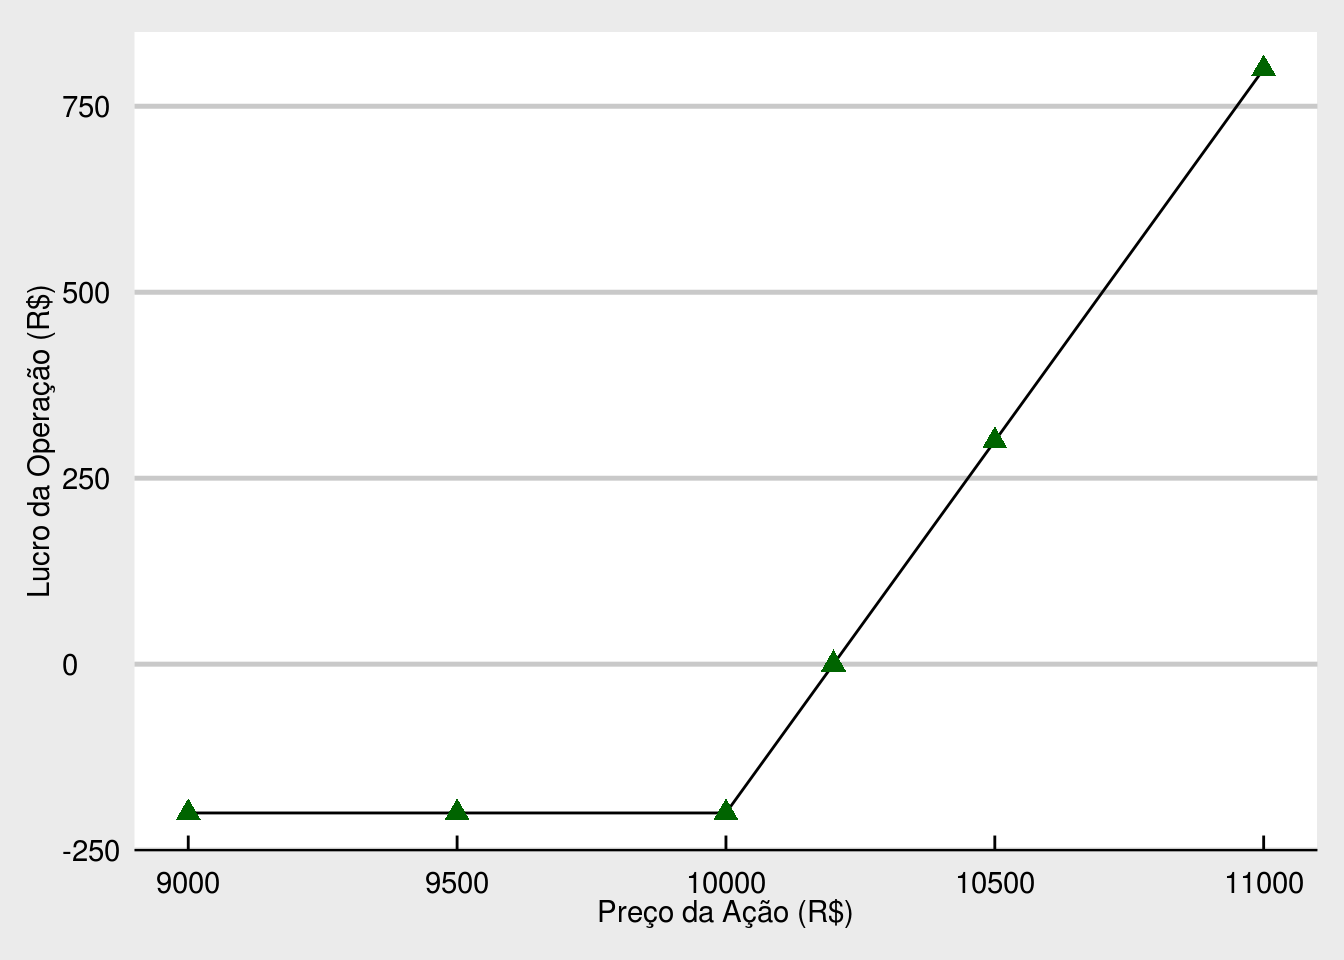
\includegraphics{01-introducao-as-opcoes_files/figure-latex/call-1.pdf}
\caption{\label{fig:call}Perfil de lucro típico de uma compra de call.}
\end{figure}

No caso de uma operação de uma compra de put, caso o preço do ativo
tenha subido acima do strike, não faz sentindo o detentor da opção
exercer seu direito, assim sua perda será apenas o valor pago pela
opção. Caso o preço do ativo tenha descido abaixo do strike, o comprador
da put pode realizar a venda e começará a lucrar a partir do momento em
que o strike fique acima do valor do ativo somado ao valor do prêmio
pago pela opção. Usando a tabela 1.2 como exemplo é possível ver que o
resultado final será de no mínimo -R\$600 caso o valor do ativo
subjacente seja igual ou maior que R\$15.000, e o resultado final
aumenta conforme o ativo perde o valor, sendo positivo a partir de
quando seu valor é de R\$14.400.

\section{Conceitos in the money, at the money e out the
money}\label{conceitos-in-the-money-at-the-money-e-out-the-money}

Estes termos são usados para se referir a opções que estão com o preço
de exercício (strike) do ativo abaixo, acima ou igual ao valor atual do
ativo.

\begin{itemize}
\tightlist
\item
  Out the money: Strike do ativo subjacente está abaixo do valor de
  mercado no caso de calls ou quando o strike do ativo está acima do
  valor de mercado no caso de puts.\\
\item
  At the money: Strike do ativo subjacente é o igual ao valor de
  mercado.
\item
  In the money: Strike do ativo subjacente está acima do valor de
  mercado no caso de calls ou quando o strike do ativo está abaixo do
  valor de mercado no caso de puts.
\end{itemize}

\section{Modelos americano e europeu de
opções}\label{modelos-americano-e-europeu-de-opcoes}

No modelo americano de opções o comprador pode exercer seu direito de
compra ou venda do ativo subjacente a qualquer momento entre o início do
contrato e o vencimento dele, enquanto isso no modelo europeu a
transação só pode ser realizada na data de vencimento.

\section{Hedge}\label{hedge}

O mercado de opções pode ser usado tanto para hedge (proteção) quanto
para especulação. O hedge é feito para limitar as possíveis perdas que
um investidor pode ter ao estar com seu patrimônio atrelado a
determinado ativo, por exemplo, para um acionista que possui ações de
determinada empresa se proteger contra uma possível queda no valor de
suas ações, ele pode comprar opções de venda at the money de suas ações
para que seu prejuízo máximo seja o prêmio.

\section{Travas}\label{travas}

Devido ao mercado de opções nos oferecer diversas possibilidades entre
call e put onde você pode estar comprado e/ou vendido irá surgir várias
posições a serem assumidas, para nos adequarmos ao quanto estamos
dispostos a encarar o risco parar atingirmos o retorno desejado. Essas
posições são conhecidas como ``Travas''.

Entendendo as travas, existem diversas estratégias, como por exemplo:
Trava de alta, trava de baixa, Long Straddle, Short Straddle, entre
outras. Mas afinal qual é o funcionamento delas? Supondo que o leitor
espere uma alta do mercado, no entanto acredite que não irá superar
determinado ponto ele poderá realizar uma Trava de alta. Onde comprará
uma opção de Call a um preço de strike X e vender outra Call com o preço
de strike Y, onde obrigatoriamente Y\textgreater{}X. Nesta operação
limitaremos o nosso ganho caso o mercado supere as nossas expectativas,
no entanto diminuiremos o custo da operação, o custo será o prêmio pago
pela opção X menos o prêmio recebido pela opção Y, para facilitar a
compreensão observemos o gráfico a seguir:

Nesse caso o valor do prêmio da compra foi de R\$30,00 enquanto a da
venda foi R\$10,00, assim limitamos nossa perda em R\$20,00, enquanto os
preços de strike da compra e da venda da call foram respectivamente
R\$250,00 e R\$300,00, fazendo o retorno máximo ser R\$30,00 que é a
diferença entre os valores de strike a serem realizados e descontado o
valor pago pelo prêmio.

Agora que o leitor já entendeu melhor o conceito da trava, vamos
explorar uma mais complexa a Long Butterfly. Aqui é realizado a compra
de uma put e call com preços de strike iguais, vendesse uma put com
preço inferior e vende alguma call com preço superior as iniciais.
Observe que pelo fato de contar com a venda de duas opções nessa
estratégia tem um custo de operação reduzido, no entanto o ideal é
utilizar em um mercado de pouca volatilidade, dado que se a volatilidade
ser alta perdesse a possibilidade de ter um ganho maior, nesse caso
recomenda o uso por exemplo de uma Long Straddle. Enfim vamos ao gráfico
para facilitar a compreensão da estratégia:

Teremos então a compra de uma put e call de strike iguais de R\$150,00 a
venda de uma put com strike inferior de R\$80, e a venda de uma call com
preço superior R\$220. Os valores exatos dos prêmios não nos interessam
no momento, porém é importante entender que teremos dois com saldos
positivos referente a nossa venda e dois negativos que advém das
compras, o resultado será nosso prejuízo máximo, olhando o gráfico nesse
caso é de R\$20,00. Pela área de retorno do gráfico podemos ver que
nosso risco está reduzido. Onde o pior cenário possível se encontra em o
preço do ativo-objeto se aproximar do valor do R\$150,00, que é onde os
contratos adquiridos não serão vantajosos em nenhuma ponta. No entanto
se o preço se aproximar de R\$220 poderemos exercer nosso direito da
compra da call inicial por R\$150,00(você terá o direito de comprar a um
preço inferior), o mesmo será valido caso haja uma queda do preço se
aproximado do valor de R\$80,00 onde a logica será a mesma só que aqui
será o usado o direito da compra da put por R\$150,00(Você terá o
direito de vender a um preço superior). Observe que apesar do nosso
risco ser reduzido, limita os nossos ganhos, com a venda da call e da
put com preços superior e inferior respectivamente.

Espero que o leitor tenha despertado interesse no assunto, com esse
conteúdo dominado já saberá o básico sobre opções, fique atento a novas
postagens em breve iremos mais a afundo explicando por exemplo o modelo
Black Scholes, como as opções são precificadas entre outros materiais.

\hypertarget{processos-estocasticos}{\chapter{Processos Estocásticos em
Finanças}\label{processos-estocasticos}}

Neste capítulo abordaremos um assunto técnico, mas muito utilizado e de
fudamental importância para a precificação de instrumentos derivativos.
Será apresentado o conceito de processos estocásticos - PE, e sua
aplicação no mundo das finanças.

Um processo estocástico é a evolução temporal de uma determinada
variável de interesse que pode assumir valores aleatórios em cada ponto
no tempo. Em outras palavras, o caminho que a variável segue ao longo do
tempo evolui de maneira incerta. Estes processos podem se dar em tempo
discreto ou em tempo contínuo. Processo em tempo discreto são aqueles
onde o valor da variável pode se alterar somente em intervalos
pré-definidos de tempo, por exemplo ao final do dia. Em processos em
tempo contínuo, o valor de nossa variável está constantemente em
mudança, de forma aleatória seguindo alguma distribuição de
probabilidades.

Estes processos são muito importantes em finanças pois, é amplamente
aceito que a evolução do preço de ativos financeiros pode ser modelado
por um PE em tempo contínuo, sendo este modelo portanto, a base para a
teoria de precificação de ativos e da qual os derivativos fazem extenso
uso. Aprender sobre a evolução temporal do preço de uma ação através de
um processo estocástico é o primeiro passo para saber como atribuir um
preço a uma opção sobre esta ação, por exemplo.

Deve ser notado também que apesar de o preço dos ativos serem
\textbf{observados} apenas em intervalos discretos de tempo (apenas
quando existe transação) e assumirem valores também discretos (múltiplos
de um centavo), o preço e sua evolução estão ocorrendo continuamente,
nossas observações que são discretas. Desta forma os processos em tempo
contínuos são ideais para este tipo de modelagem.

\section{Processos de Markov}\label{markov}

Uma primeira definição de deve-se fazer para estudar PE aplicados a
evolução do preço de ações é o conceito de processo de Markov. Este tipo
de processo é tal que o histórico do processo que o levou até seu estado
atual, é \textbf{irrelevante} para a previsão de seu estado futuro. Ou
seja, toda a informação da história do processo já está contida no seu
valor atual. Quando consideramos que preços de ativos seguem um processo
de Markov, estamos assumindo válida pelo menos a forma fraca de mercados
eficientes.

Uma implicação desta suposição, verificada empiricamente, é que não se
pode obter lucros apenas seguindo padrões históricos do preço e
extrapolando-os no futuro. Outra, mais importante para nossos processos,
é que as distribuições de probabilidade que a variável aleatória segue
em cada ponto no tempo são \textbf{independentes}.

\section{Movimento Browniano}\label{mb}

Suponha um processo de Markov, que para fins de simplificação
consideraremos em tempo discretos. Se a distribuição de probabilidade
para o próximo incremento no valor do processo for uma Normal com média
zero e variância unitária, podemos representar este incremento por
\(\phi(0, 1)\). Como este é um processo de Markov, o segundo incremento
será independente do primeiro e terá novamente a mesma distribuição de
probabilidade. Qual seria então, a partir do período inicial até o
segundo período, a distribuição de probabilidade dos possíveis valores
de nosso hipotético processo? A reposta é a soma de duas normais
\(\phi(0, 1)\) que resulta em \(\phi(0, 2)\). Se assim continuarmos a
fazer previsões para T períodos a frente, nossa distribuição terá
densidade \(\phi(0, T)\).

Para tempos discretos, \(T\in\mathbb{Z}\) este é o processo do passeio
aleatório (\emph{Random Walk}), entretanto para tempo contínuo quando
\(T\in\mathbb{R}\) com incrementos acontecendo em intervalos de tempo
infinitesimalmente pequenos, este é o Movimento Browniano - MB, que
também é largamente conhecido como processo de Wiener.

\begin{Shaded}
\begin{Highlighting}[]
\NormalTok{t <-}\StringTok{ }\DecValTok{0}\OperatorTok{:}\DecValTok{500}
\NormalTok{m <-}\StringTok{ }\DecValTok{5} \CommentTok{# Numero de simulacoes}
\NormalTok{mc_names <-}\StringTok{ }\KeywordTok{paste0}\NormalTok{(}\StringTok{"Sim"}\NormalTok{, }\KeywordTok{seq_len}\NormalTok{(m)) }\CommentTok{# Nomes das simulacoes}
\NormalTok{sigma2 <-}\StringTok{ }\DecValTok{1}
\NormalTok{mu <-}\StringTok{ }\DecValTok{0}
\NormalTok{brown_t <-}\StringTok{ }\KeywordTok{matrix}\NormalTok{(}\DataTypeTok{nrow =} \KeywordTok{length}\NormalTok{(t), }\DataTypeTok{ncol =}\NormalTok{ m)}
\CommentTok{# MC Simulation}
\KeywordTok{set.seed}\NormalTok{(}\DecValTok{543210}\NormalTok{)}
\ControlFlowTok{for}\NormalTok{ (i }\ControlFlowTok{in} \KeywordTok{seq_len}\NormalTok{(m)) \{}
\NormalTok{  increments <-}\StringTok{ }\KeywordTok{rnorm}\NormalTok{(}\KeywordTok{length}\NormalTok{(t) }\OperatorTok{-}\StringTok{ }\DecValTok{1}\NormalTok{, mu, }\KeywordTok{sqrt}\NormalTok{(sigma2))}
\NormalTok{  brown_t[, i] <-}\StringTok{ }\KeywordTok{c}\NormalTok{(}\DecValTok{0}\NormalTok{, }\KeywordTok{cumsum}\NormalTok{(increments))}
\NormalTok{\}}

\KeywordTok{colnames}\NormalTok{(brown_t) <-}\StringTok{ }\NormalTok{mc_names}
\NormalTok{mb <-}\StringTok{ }\KeywordTok{as.tibble}\NormalTok{(}\KeywordTok{cbind}\NormalTok{(t, brown_t)) }\OperatorTok\StringTok{ }
\StringTok{  }\KeywordTok{gather}\NormalTok{(}\DataTypeTok{key =}\NormalTok{ sim, }\DataTypeTok{value =}\NormalTok{ value, }\OperatorTok{-}\NormalTok{t)}
\end{Highlighting}
\end{Shaded}

\begin{verbatim}
## Warning: `as.tibble()` is deprecated, use `as_tibble()` (but mind the new semantics).
## This warning is displayed once per session.
\end{verbatim}

\begin{Shaded}
\begin{Highlighting}[]
\KeywordTok{ggplot}\NormalTok{(mb, }\KeywordTok{aes}\NormalTok{(}\DataTypeTok{x =}\NormalTok{ t, }\DataTypeTok{y =}\NormalTok{ value, }\DataTypeTok{color =}\NormalTok{ sim)) }\OperatorTok{+}\StringTok{ }
\StringTok{  }\KeywordTok{geom_line}\NormalTok{() }\OperatorTok{+}
\CommentTok{#  geom_point(data = dens_tbl, aes(x = x, y = y), size = 1) +}
\StringTok{  }\KeywordTok{labs}\NormalTok{(}\DataTypeTok{title =} \StringTok{"5 realizações Movimento Browniano"}\NormalTok{,}
       \DataTypeTok{x =} \StringTok{"Tempo"}\NormalTok{,}
       \DataTypeTok{y =} \StringTok{"Valor"}\NormalTok{) }\OperatorTok{+}
\StringTok{  }\KeywordTok{guides}\NormalTok{(}\DataTypeTok{color =} \OtherTok{FALSE}\NormalTok{) }\OperatorTok{+}
\StringTok{  }\KeywordTok{scale_color_viridis_d}\NormalTok{() }\OperatorTok{+}
\StringTok{  }\KeywordTok{theme_economist_white}\NormalTok{()}
\end{Highlighting}
\end{Shaded}

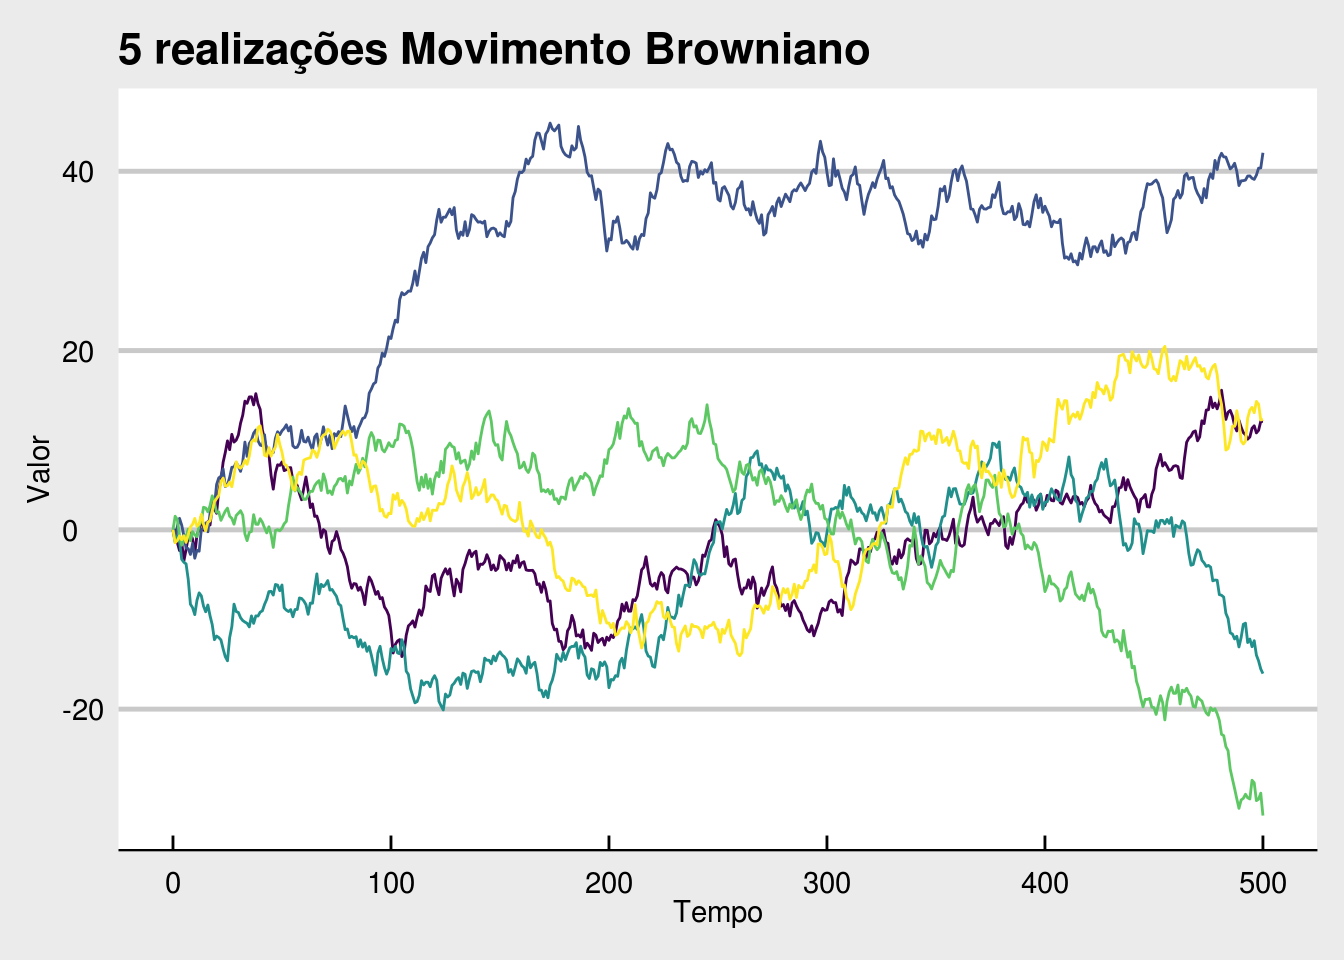
\includegraphics{02-processos-estocasticos-em-financas-uma-introducao_files/figure-latex/brownian_plot-1.pdf}

A figura acima mostra 5 realizações de um \emph{mesmo} processo
estocástico com média zero e variância unitária. É importante frisar que
o processo que gerou as cinco séries é exatamente o mesmo, sendo elas
tão distintas umas das outras ou não. Esta é uma importante
característica dos processos estocásticos nas aplicações reais, o que
nós observamos é apenas uma realização do processo, dentre as infinitas
possíveis.

\section{Definição}\label{definicao}

Agora que já foi passada a intuição sobre processos estocásticos,
pode-se partir para definições mais formais sobre estes processos. Vamos
adotar a notação do cálculo para tanto, e generalizar nosso MB
possibilitando-o que tenha média diferente de zero (\(\mu\)) e variância
qualquer (\(\sigma^2\)), mantendo estas constantes ao longo do tempo,
entretanto. Desta forma um movimento Browniano com deriva pode ser
descrito através da seguinte equação diferencial estocástica - EDE:

\begin{equation}
dX_t = \mu dt + \sigma dB_t
\label{eq:mb}
\end{equation}

onde \(dB_t\) é nosso MB padrão em um intervalo de tempo infinitesimal,
\(dt\).

O processo \(X_t\) possui uma taxa de deriva (média instantânea) igual a
\(\mu\) e volatilidade instantânea igual a \(\sigma\). Quando um PE
possui deriva igual a zero, como nosso MB padrão, o valor esperado deste
processo para qualquer período futuro será zero. Este fato deixa de ser
verdade no processo generalizado, com taxa de deriva diferente de zero.
Neste caso o processo evoluirá seguindo uma taxa crescente (se
\(\mu > 0\)) ou decrescente (se \(\mu < 0\)). Assim é possível, a partir
de um MB padrão, modelar outros PE que possuam tendência temporal e
variâncias diferentes.

\section{Movimento Browniano Geométrico}\label{mbg}

Apesar de o processo \(X_t\) ser bastante flexível e cobrir uma grande
gama de usos, ele ainda não é adequado para modelar o preço de ativos, e
isto se dá em função de o processo de Wiener, mesmo com deriva positiva,
poder atingir valores negativos com probabilidade maior que zero. Isto
implicaria na possibilidade do preço de uma ação ser negativo, algo que
obviamente não ocorre. Além desta impossibilidade, existe um outro
empecilho para se utilizar o MB para modelar o processo de preços, e
este é a deriva constante \(\mu\) com relação ao preço da ação.

A deriva pode ser interpretada como o valor esperado do retorno da ação
em um dado período de tempo. Este retorno esperado ele é pode ser
constante em termos percentuais (em um modelo simplificado), mas não em
termos absolutos! Ou seja, dependendo do preço da ação, R\$ 1,00 ou R\$
100,00, a deriva \(\mu\) deve ser diferente para que em termos
percentuais a relação seja constante.

A solução para estes dois problemas é modelar o preço como um processo
estocástico conhecido como Movimento Browniano Geométrico. Ele difere do
MB padrão pois assume que o \textbf{logaritmo} da variável aleatória
possui distribuição Normal. O MBG é a resolução para a seguinte EDE:

\begin{equation}
dX_t = \mu X_t dt + \sigma X_t dB_t
\label{eq:mbg}
\end{equation}

Veja que este é basicamente o mesmo processo MB, porém a deriva, termo
que multiplica \(dt\), varia linearmente com o valor do processo
(\(\mu X_t\)) assim como a volatilidade instantânea (\(\sigma X_t\)).

A solução para esta EDE, para um valor inicial qualquer de \(X\)
(\(X_0 > 0\)) é dada por:

\begin{equation}
X_t = X_0\exp\left(\left(\mu-\frac{\sigma^2}{2}\right)t+\sigma B_t\right)
\label{eq:mbgsol}
\end{equation}

A variável aleatória \(X\) segue um MB ao longo de uma trajetória
exponencial. É fácil verificar que, por ser exponencial, \(X_t\) nunca
terá valor negativo.

Esta é uma forma conveniente de representar a evolução de preços de um
ativo pois naturalmente surge o conceito de retornos logarítmos. O
log-retorno de \(X\) é dado por \(r_t=\ln(X_t/X_0)\) de onde inferimos
que se o processo de formação de preço de um ativo segue um MBG, então
seus log-retornos serão normalmente distribuídos com média
\(\mu-\frac{\sigma^2}{2}\) e volatilidade \(\sigma\) em uma unidade de
período considerado. Se escalarmos o período de tempo considerado para
\(T\), temos então que os retornos logarítmicos do ativo \(X\) seguem a
seguinte distribuição normal:

\begin{equation}
r_T \sim\phi\left(\left(\mu-\frac{\sigma^2}{2}\right)T, \sigma^2T\right)
\label{eq:rT}
\end{equation}

Abaixo apresentamos 5 realizações de um MBG com valor de deriva
\(\mu = 0,6\% a.p.\) e variância \(\sigma^2=1\% a.p.\).

\begin{Shaded}
\begin{Highlighting}[]
\NormalTok{t <-}\StringTok{ }\DecValTok{0}\OperatorTok{:}\DecValTok{500}
\NormalTok{m <-}\StringTok{ }\DecValTok{5} \CommentTok{# Numero de simulacoes}
\NormalTok{mc_names <-}\StringTok{ }\KeywordTok{paste0}\NormalTok{(}\StringTok{"Sim"}\NormalTok{, }\KeywordTok{seq_len}\NormalTok{(m)) }\CommentTok{# Nomes das simulacoes}
\NormalTok{sigma2 <-}\StringTok{ }\FloatTok{0.01}
\NormalTok{mu <-}\StringTok{ }\FloatTok{0.006} \CommentTok{# c(0.098, 0.099, 0.1, 0.101, 0.102) / 10}
\NormalTok{brown_t <-}\StringTok{ }\KeywordTok{matrix}\NormalTok{(}\DataTypeTok{nrow =} \KeywordTok{length}\NormalTok{(t), }\DataTypeTok{ncol =}\NormalTok{ m)}
\CommentTok{# MC Simulation}
\KeywordTok{set.seed}\NormalTok{(}\DecValTok{1234567}\NormalTok{)}
\ControlFlowTok{for}\NormalTok{ (i }\ControlFlowTok{in} \KeywordTok{seq_len}\NormalTok{(m)) \{}
\NormalTok{  log_ret <-}\StringTok{ }\KeywordTok{rnorm}\NormalTok{(}\KeywordTok{length}\NormalTok{(t) }\OperatorTok{-}\StringTok{ }\DecValTok{1}\NormalTok{, mu }\OperatorTok{-}\StringTok{ }\NormalTok{(sigma2 }\OperatorTok{/}\StringTok{ }\DecValTok{2}\NormalTok{), }\KeywordTok{sqrt}\NormalTok{(sigma2))}
\NormalTok{  brown_t[, i] <-}\StringTok{ }\KeywordTok{c}\NormalTok{(}\DecValTok{1}\NormalTok{, }\KeywordTok{cumprod}\NormalTok{(}\KeywordTok{exp}\NormalTok{(log_ret)))}
\NormalTok{\}}

\KeywordTok{colnames}\NormalTok{(brown_t) <-}\StringTok{ }\NormalTok{mc_names}
\NormalTok{mb <-}\StringTok{ }\KeywordTok{as.tibble}\NormalTok{(}\KeywordTok{cbind}\NormalTok{(t, brown_t)) }\OperatorTok\StringTok{ }
\StringTok{  }\KeywordTok{gather}\NormalTok{(}\DataTypeTok{key =}\NormalTok{ sim, }\DataTypeTok{value =}\NormalTok{ value, }\OperatorTok{-}\NormalTok{t)}
  
\KeywordTok{ggplot}\NormalTok{(mb, }\KeywordTok{aes}\NormalTok{(}\DataTypeTok{x =}\NormalTok{ t, }\DataTypeTok{y =}\NormalTok{ value, }\DataTypeTok{color =}\NormalTok{ sim)) }\OperatorTok{+}\StringTok{ }
\StringTok{  }\KeywordTok{geom_line}\NormalTok{() }\OperatorTok{+}
\StringTok{  }\KeywordTok{labs}\NormalTok{(}\DataTypeTok{title =} \StringTok{"5 realizações Movimento Browniano Geométrico"}\NormalTok{,}
       \DataTypeTok{x =} \StringTok{"Tempo"}\NormalTok{,}
       \DataTypeTok{y =} \StringTok{"Valor"}\NormalTok{) }\OperatorTok{+}
\StringTok{  }\KeywordTok{guides}\NormalTok{(}\DataTypeTok{color =} \OtherTok{FALSE}\NormalTok{) }\OperatorTok{+}
\StringTok{  }\KeywordTok{scale_y_continuous}\NormalTok{(}\DataTypeTok{breaks =} \DecValTok{0}\OperatorTok{:}\DecValTok{10}\NormalTok{) }\OperatorTok{+}
\StringTok{  }\KeywordTok{scale_color_viridis_d}\NormalTok{() }\OperatorTok{+}
\StringTok{  }\KeywordTok{theme_economist_white}\NormalTok{()}
\end{Highlighting}
\end{Shaded}

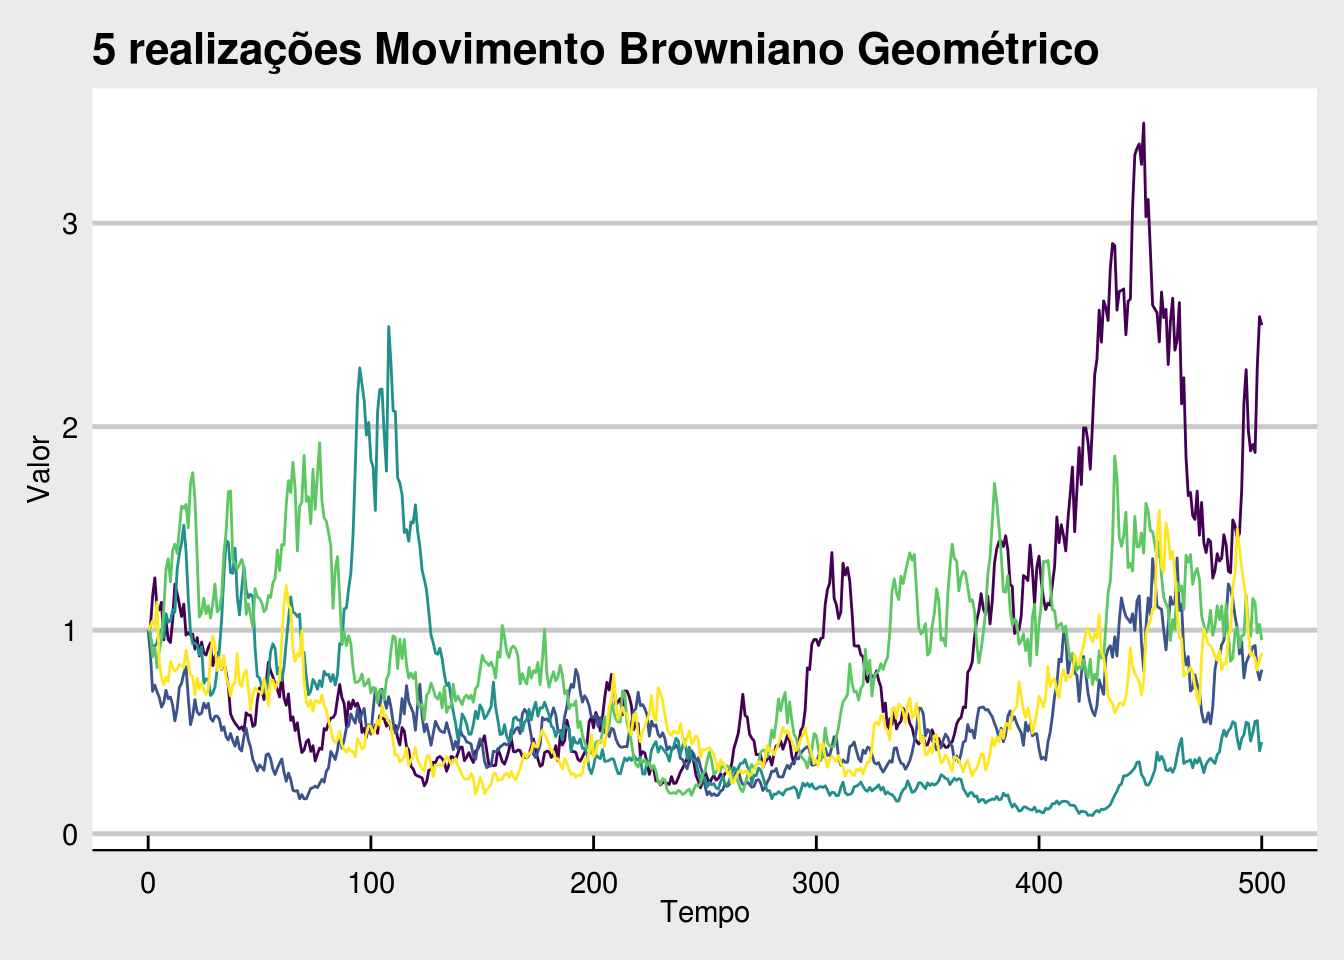
\includegraphics{02-processos-estocasticos-em-financas-uma-introducao_files/figure-latex/mbg_plot-1.pdf}

O Movimento Browniano Geométrico aqui demonstrado serve de base para o
famoso modelo \textbf{Black \& Scholes} de precificação de opções, o
qual assume que o ativo subjacente à opção (por exemplo, a ação de uma
empresa) tem seu preço formado por um processo MBG.

\hypertarget{bsm}{\chapter{Modelo Black-Scholes-Merton}\label{bsm}}

Neste capítulo desenvolveremos o modelo para precificação de opções do
tipo europeias proposto \citet{Black1973} e posteriormente expandido por
\citet{Merton1976}. A derivação deste modelo se baseia nos conceitos
apresentados sobre processos estocásticos do Capítulo
\ref{processos-estocasticos}.

Antes de entrar na modelagem desenvolvida pelos autores acima citados,
iremos tratar de algumas definições essenciais, como por exemplo a
precificação de ativos em um mundo neutro ao risco (\emph{risk neutral
valuation}) e portfólio de replicação (\emph{replicating portfolio}),
que são largamente utilizados na precificação de quaisquer derivativos,
e não somente opções.

\section{Portfólio de replicação}\label{portfolio-de-replicacao}

Suponha que se deseja precificar uma opção de compra sobre uma ação,
vamos denotar o preço desta \emph{call} de \(f_t\). Sabemos que na data
de expiração, \(T\), da opção de compra seu preço será:
\(f_T=max(S_T - K, 0)\), onde \(S_T\) é o preço da ação subjacente na
data \(T\) e \(K\) é o preço de exercício da opção. Podemos criar um
portfólio que envolva um ativo livre de risco, com preço \(B_t\) e a
ação objeto do derivativo, \(S_t\), que recrie o mesmo valor de
pagamento que a opção na data de expiração. Ou seja, criamos o portfólio
de replicação \(P_t=\Delta S_t + b B_t\), no qual devemos escolher os
valores de \(\Delta\) e \(b\) de tal forma que \(f_T = P_T\).

De fato, para apenas um período a frente, podemos tomar emprestado a
taxa de juros livre de risco\footnote{Esta é uma suposição do modelo,
  pode não ser verdade para algum investidor qualquer mas se for para
  algum outro investidor representativo, o princípio de ausência de
  arbitragem passa a valer, uma vez que este segundo investidor
  explorará o mercado e levará o preço do derivativo para o resultado
  requerido.}, \(r\) um valor igual ao preço corrente da ação, \(S_0\) e
comprá-la, ao mesmo tempo em que se ``trava'' (faz \emph{hedge}) deste
portfólio vendendo a opção. O lucro desta operação em \(T\) deve ser
zero, pois é um portfólio travado. Com estas premissas é possível
calcular o preço do prêmio da opção a ser cobrado no período inicial
para que o valor esperado da operação como um todo seja zero.

Este portfólio formado pela venda do ativo livre de risco e compra do
ativo objeto é denominado \emph{portfólio de replicação}, pois, ele
fornece um fluxo de caixa igual ao derivativo que buscamos precificar.
Ao adicionarmos ao portfólio de replicação a venda (ou seja, o negativo)
do derivativo, temos um portfólio \emph{hedgeado}, onde não existe mais
incerteza com relação ao seu retorno esperado.

\section{Precificação neutra ao
risco}\label{precificacao-neutra-ao-risco}

A metodologia de precificação de derivativos dentro do \emph{mundo
neutro ao risco}\footnote{A precificação dentro do mundo neutro ao risco
  mereceria um, ou mais, \emph{posts} por si só. Aqui lançaremos apenas
  os principais resultados que nos permitem encontrar o modelo de B\&S.}
é o carro-chefe das metodologias para se avaliar estes instrumentos. O
princípio de precificação neutra ao risco afirma que um derivativo pode
ser valorado através das seguintes suposições:

\begin{itemize}
\tightlist
\item
  o retorno esperado do ativo objeto é a taxa livre de risco, e
\item
  o valor esperado do derivativo na expiração deve ser descontado pela
  taxa livre de risco para trazê-lo a valor presente.
\end{itemize}

É claro que o mundo real não é neutro ao risco, entretanto uma das
provas que a metodologia faz é que, ao precificarmos um derivativo de
forma relativa ao preço do ativo objeto, a precificação neutra ao risco
encontra o mesmo valor para o derivativo que uma metodologia que leve em
conta as preferências ao risco dos investidores. Entretanto, precificar
um derivativo assumindo neutralidade ao risco é muito mais simples que
encarar um modelo baseado no mundo real.

De fato a neutralidade ao risco soa um tanto quanto estranha a primeira
vez. Porém, ela tem uma explicação lógica de sua validade nas
circunstâncias em que é desenvolvida. Se os investidores forem avessos
ao risco, por exemplo, os retornos esperados para o ativo objeto terão
embutidos um prêmio pelo risco. Acontece que este prêmio pelo risco
também deverá estar na taxa de desconto do valor esperado de pagamento
do derivativo, de forma que este prêmio ao risco é cancelado.

É comum na literatura de derivativos encontrarmos os termos mundo-P e
mundo-Q. O mundo-P se refere ao mundo real, com probabilidades P reais
de ocorrência de eventos, equanto que o mundo-Q é o mundo neutro ao
risco, onde as probabilidades Q são ajustadas (tecnicamente suas medidas
são alteradas) para refletir esta neutralidade. No mundo-Q é comum
denotarmos o valor esperado de alguma variável aleatória com a seguinte
notação: \(\mathbb{E_Q}[\cdot]\).

Assim, a precificação de derivativos supondo um mundo neutro ao risco
chega no preço correto para todos os mundos.

\section{Encontrando a equação de
Black-Scholes}\label{encontrando-a-equacao-de-black-scholes}

Vamos partir do princípio que nossa ação, objeto da opção que desejamos
precificar, siga um MBG conforme descrito no
\protect\hyperlink{processos-estocasticos}{capítulo anterior}. Portanto,
o preço de nossa ação no período \(t\) deve observar a seguinte equação
diferencial estocástica:

\begin{equation}
dS_t=\mu S_t+\sigma S_t dW_t 
\label{eq:ds}
\end{equation}

onde \(dW_t\) é o movimento Browniano, ou processo de Wiener.

Esta equação resume as principais hipóteses do modelo Black\&Scholes de
precificação de opções, são elas:

\begin{itemize}
\tightlist
\item
  O preço do ativo objeto é um processo estocástico e segue uma
  distribuição log-normal;
\item
  O retorno esperado (\(\mu\)) e a volatilidade (\(\sigma\)) deste ativo
  são \textbf{constantes}, tanto no tempo quanto com relação ao próprio
  nível de preço do ativo objeto.
\end{itemize}

Ademais destas hipóteses, temos aquelas relacionadas a racionalidade dos
mercados e ao princípio de ausência de oportunidades de arbitragem.
Estas hipóteses nos levam a validade do mundo neutro ao risco e
portanto, a resolução do modelo da forma como descreveremos abaixo.

Nossa opção será descrita por um portfólio de replicação, e se tomarmos
seu preço no instante \(t\), então a opção também deve seguir uma
equação diferencial estocástica da forma:

\begin{equation}
df_t=\Delta dS_t+b\,dB_t 
\label{eq:df1}
\end{equation}

aqui \(dB_t\) representa a variação do ativo livre de risco (dinheiro)
dentro de um período de tempo \(dt\). Sabemos que o valor do ativo livre
de risco não envolve incerteza alguma, é determinístico, e seu
rendimento é a taxa de juros livre de risco. Assim, para uma taxa
continuamente composta \(r\) uma unidade de \(B\) evolui através de
\(B_t=e^{rt}\), logo:

\begin{equation}
dB_t=rBdt
\label{eq:db}
\end{equation}

De acordo com o
\href{https://pt.wikipedia.org/wiki/Lema_de_It\%C5\%8D}{lema de Ito} o
diferencial de uma função que dependa do tempo e de um processo
estocástico pode ser encontrado da seguinte forma:

\begin{equation}
df_t=\frac{\partial f}{\partial t}dt + \frac{\partial f}{\partial S}dS + \frac{1}{2}\frac{\partial^2 f}{\partial S^2}dS^2
\label{eq:df2}
\end{equation}

onde \(dS^2\) é a variação quadrática de nosso processo \(S_t\) que é um
movimento browniano geométrico, logo \(dS^2=\sigma^2S^2dt\).

Igualando as equações \eqref{eq:df1} e \eqref{eq:df2}, fazendo as devidas
substituições trazidas pelas equações \eqref{eq:ds} e \eqref{eq:db} e por
fim rearranjando os termos, chegamos na seguinte relação:

\begin{equation}
\left( \frac{\partial f}{\partial t} + \frac{\partial f}{\partial S}\mu S + \frac{1}{2}\frac{\partial^2 f}{\partial S^2}\sigma^2 S^2 - \Delta\mu S - rbB \right)dt + \left( \frac{\partial f}{\partial S}\sigma S - \Delta \sigma S \right)dW = 0 
\end{equation}

que para ser válida para todo \(t\), cada termo entre parênteses deve
ser igual a zero simultaneamente. Rapidamente chegamos aos valores
necessários de nosso portfólio de replicação.

\begin{equation}
\Delta = \frac{\partial f}{\partial S} 
\label{eq:delta}
\end{equation}

\begin{equation}
rbB = \frac{\partial f}{\partial t}+\frac{1}{2}\frac{\partial^2 f}{\partial S^2}\sigma^2S^2 
\label{eq:rbb1}
\end{equation}

Através da equação \eqref{eq:df1}, integrando-a, chegamos na relação
\(bB = f - \Delta S\) e pré-multiplicando ambos os lados por \(r\) temos
então que:

\begin{equation}
rbB = r(f-\Delta S) 
\label{eq:rbb2}
\end{equation}

Finalmente, igualando as equações \eqref{eq:rbb1} e \eqref{eq:rbb2} e
substituindo o valor de \(\Delta\) encontramos a famigerada equação
diferencial parcial - EDP - de Black\&Scholes:

\begin{equation}
\frac{\partial f}{\partial t}+\frac{1}{2}\sigma^2S^2\frac{\partial^2 f}{\partial S^2}+rS\frac{\partial f}{\partial S} - rf = 0
\label{eq:BS}
\end{equation}

\section{Solução analítica}\label{solucao-analitica}

A equação possui diferentes formas de resolução\footnote{Uma
  demonstração completa de como encontrar a solução para a EDP de
  Black\&Schole pode ser encontrada em
  \url{https://planetmath.org/AnalyticSolutionOfBlackScholesPDE}}, a
precificação do derivativo irá depender da forma que resolvermos a
equação \eqref{eq:BS}. O Modelo Black\&Scholes é famoso por conseguir
precificar opções call e put europeias, onde a resolução da equação fará
uso dos \emph{payoffs}. Para uma call:

\begin{equation}
\displaystyle f(S,T)=\max(S-K,0)
\label{eq:cpayoff}
\end{equation}

Já no caso de uma put:

\begin{equation}
\displaystyle f(S,T)=\max(K-S,0)
\label{eq:ppayoff}
\end{equation}

Onde:

\begin{itemize}
\tightlist
\item
  T é a data de vencimento da opção,
\item
  K é o preço de exercício, e
\item
  S é o preço do ativo subjacente.
\end{itemize}

Utilizando os \emph{payoffs} dados nas equações \eqref{eq:cpayoff} e
\eqref{eq:ppayoff}, e resolvendo a EDP de Black\&Scholes \eqref{eq:BS},
iremos obter o modelo para se precificar os derivativos citados.

Para uma Call temos que:

\begin{equation}
C(S,t)=SN(d_{1})-Ke^{-r(T-t)}N(d_{2})
\label{eq:call}
\end{equation}

Já para um Put chegamos a:

\begin{equation}
P(S,t)=Ke^{-r(T-t)}N(-d_{2})-SN(-d_{1})
\label{eq:put}
\end{equation}

onde:

\begin{equation}d_{1}={\frac {\ln(S/K)+(r+\sigma ^{2}/2)(T-t)}{\sigma {\sqrt {T-t}}}}
\label{eq:d1}
\end{equation}

\begin{equation}d_{2}={\frac {\ln(S/K)+(r-\sigma ^{2}/2)(T-t)}{\sigma {\sqrt {T-t}}}}=d_1-\sigma\sqrt{T-t}
\label{eq:d2}
\end{equation}

É a partir das equações \eqref{eq:call} e \eqref{eq:put} que se obtém as
chamadas gregas, que são as sensibilidades do preço do derivativo em
relação a alterações nos parâmetros do modelo. Explicaremos as gregas em
maiores detalhes mais adiante.

\section{Paridade compra e venda}\label{putcallparity}

Agora vamos falar um pouco sobre a paridade entre opções de compra e
venda, algo que nos ajuda a precificar algum derivativo quando já
conhecemos o preço de outro derivativo com especificações semelhantes.

Assumindo ausência de oportunidade de arbitragem, com um ativo
subjacente que tenha liquidez, iremos verificar a paridade Call-Put que
define uma relação entre os preços de uma call e put do tipo europeu,
desde que possuam o \textbf{mesmo tempo de maturidade} e \textbf{preço
de strike}. Aqui possuiremos menos premissas que o modelo Black\&Scholes
e premissas mais simples, tal relação poderá ser utilizada para
encontrar o valor justo de uma opção. Com a ausência de arbitragem
observe que dois portfolios que sempre geram o mesmo payoff em um
instante T devem ter o mesmo valor em qualquer instante intermediário.

Imagine um primeiro portfólio onde o investidor compre uma opção de
compra C, a qual possui tempo de maturidade T e preço de strike K, sobre
algum ativo subjacente que chamaremos de S e compre um título B que seu
valor no período T seja de {\$}30. E um segundo portfolio onde tenha o
próprio ativo subjacente S que esteja sendo negociado a {\$}25 e compre
uma put P com um preço de strike K e maturidade T. Estes são porfólios
de replicação entre si, eles terão exatamente o mesmo \emph{payoff} no
período T, e na ausência de arbitragem, podemos calcular seus retornos
através da precificação neutra ao risco. Teremos uma relação onde os
valores dos nossos portfolios serão:

\begin{equation}
\mathbb{E_Q}[S_t + P_t] = \mathbb{E_Q}[C_t + B_t]; \quad t \leq T
\label{eq:parity}
\end{equation}

Como estamos em um mundo neutro ao risco, \(P_t\) e \(C_t\) são os
preços da put e da call dados pelo modelo B\&S, enquanto
\(\mathbb{E_Q}[B_t]\) se resume a \(Ke^{-r(T-t)}\), ou seja, a posição
atual em ativo livre de risco deve ser o valor presente do strike das
opções. O preço do subjacente é o próprio preço atualmente observado.

Como \(S_t\) e \(B_t=Ke^{-r(T-t)}\) são conhecidos, se no mercado
existir um preço \(C_t\) então podemos calcular \(P_t\) e vice-versa.
Esta é a essência da paridade compra e venda.

Observe que se essa relação não for mantida, teremos arbitragem:
Suponhamos que \(S_t > B_t\) e que a put esteja com um premio mais alto
que a call no entanto ambos possuem um preço de strike {\$}30 e
maturidade T, que os prêmios sejam {\$}20 e {\$}15 respectivamente
teremos então: 30 + 20 = 15 + 25, nesse caso teremos 50 \(\neq\) 40,
então vende-se o que está mais caro, no caso a ação e a put e compraria
o título e a call, chegando ao um lucro de 50-40=10, de {\$}10 sem
risco. Observe que independentemente de a ação subir acima ou cair
abaixo do strike, o lucro obtido nesta operação será sempre de {\$}10.

\section{As Gregas}\label{gregas}

As letras gregas utilizadas no mercado de opções são usadas para denotar
as sensibilidades do preço da opção com relação a variação de alguma das
variáveis do modelo, a seguir entraremos em detalhes sobre as principais
gregas usadas para a análise de opções.

\subsection{Delta}\label{delta}

Já havíamos definido o delta anteriormente ao encontrarmos a EDP de
Black\&Scholes, isto é:

\begin{equation}
\Delta = \frac{\partial f}{\partial S}
\label{eq:delta}
\end{equation}

O delta mede a taxa com que o preço da opção muda conforme o valor do
ativo subjacente oscila, seu valor pode variar entre 1 e 0 para call e
entre 0 e -1 para put.

Exemplo: imagine uma opção de compra de 100 ações que possui um delta de
0,72, caso o ativo subjacente aumente {\$}1 o valor da opção aumentará
{\$}72 (pois representa 100 ações), e caso o valor do ativo subjacente
diminua o preço da opção diminuirá {\$}72.

O mesmo acontece com opções de venda, só que de uma forma inversamente
proporcional pelo seu delta ser negativo. Uma opção de venda de 100
ações que possui um delta de -0,40 vai valer menos {\$}40 caso o preço
do seu ativo subjacente aumente {\$}1, e vai valer mais {\$}40 caso o
preço do seu ativo subjacente diminua {\$}1.

O strike da opção influência o delta diretamente, quanto mais
in-the-money for uma opção, call ou put, maior será o seu delta em valor
absoluto, e quanto mais out-the-money, menor será o módulo de seu delta.

\subsection{Gamma}\label{gamma}

\begin{equation}
\Gamma = \frac{\partial \Delta}{\partial S} = \frac{\partial^2 f}{\partial S^2}
\label{eq:gamma}
\end{equation}

O gamma mede a taxa com que o delta muda a cada oscilação do preço do
ativo subjacente, seu impacto aumenta conforme o valor atual do ativo se
aproxima do strike, sendo responsável pela convexidade do valor da
opção. Opções de alto gamma são chamadas de explosivas, uma vez que
mesmo pequenas variações no preço do ativo se traduzem em grandes
oscilações no preço da opção.

\subsection{Theta}\label{theta}

\begin{equation}
\Theta = -\frac{\partial f}{\partial \tau}, \quad \tau=T-t
\label{eq:theta}
\end{equation}

O Theta é uma taxa que mede o efeito do tempo sobre o preço da opção.
Como as opções tem um maior valor de acordo com a quantidade de tempo
até a data de vencimento, seu valor também diminui conforme o tempo
passa, theta é a letra que mede essa variação (que sempre é negativa). O
valor de theta representa a quantidade de dinheiro perdida no prêmio da
opção a cada dia que passa.

\subsection{Vega}\label{vega}

\begin{equation}
\displaystyle {\mathcal {V}}=\frac{\partial f}{\partial \sigma} 
\label{eq:vega}
\end{equation}

O vega é uma taxa que mede o efeito da mudança da volatilidade no preço
da opção. Seu valor é praticamente constante em opções com a mesma data
de vencimento, esse valor aumenta em datas de vencimento mais distantes
devido ao maior espaço de tempo em que a volatilidade atua, devido ao
maior intervalo de tempo que há para ocorrer mudanças nos preços.

\subsection{Rho}\label{rho}

\begin{equation}
\displaystyle \rho =\frac{\partial f}{\partial r}
\label{eq:rho}
\end{equation}

O rho é uma taxa que mede a sensitividade do preço da ação em relação à
taxa livre de risco, caso o valor de de rho determinada opção seja 0,7,
para cada aumento de 1\% da taxa livre de risco o valor da opção
aumentará 0,7\%. Essa taxa influi principalmente no preço de opções com
uma data de vencimento extremamente distante, não afetando muito o preço
de opções cuja data de vencimento é próxima.

\hypertarget{smile}{\chapter{Smile de Volatilidade}\label{smile}}

A volatilidade instantânea, \(\sigma\), do ativo subjacente é a única
variável no modelo B\&S que não pode ser diretamente observada. De fato,
a volatilidade (ou equivalentemente a variância) de um ativo é dita uma
variável \textbf{latente}. Sabemos que ela existe e possui algum valor
no processo gerador, o processo pelo qual os preços são formados, porém
não conseguimos observá-la diretamente, apenas estimá-la. Uma das formas
de estimação de volatilidade pode ser a partir de dados históricos, mas
várias outras formas existem, entre elas processos GARCH, volatilidade
realizada, volatilidade estocástica, etc.

Uma vez que a volatilidade não pode ser diretamente observada, a prática
comum no mercado é fazer o caminho inverso. Considerar os preços de
mercado para as opções como dado, e a partir do modelo
\protect\hyperlink{bsm}{B\&S} inverter a equação de preço da Call ou Put
para encontrar a volatilidade deste modelo que é compatível com os
preços de mercado. A esta volatilidade encontrada damos o nome de
\textbf{volatilidade implícita}.

Portanto, o smile de volatilidade que tratamos neste post é na verdade
um gráfico entre a volatilidade implícita, retirada de opções Européias
(baunilhas, do inglês vanilla options) a partir do modelo B\&S, contra
os \emph{strikes} destas opções.

\section{Reparametrizando B\&S e definição de
moneyness}\label{reparametrizando}

Nem sempre é interessante plotar o smile contra os \emph{strikes}
propriamente ditos, uma forma de avaliar o quanto uma opção está
``dentro, fora ou no dinheiro'' pode ser a grega Delta ou então o
chamado \emph{moneyness} (por favor, se alguém tiver uma boa tradução
para este termo, deixe nos comentários). Tradicionalmente a medida de
\emph{moneyness} é a relação \(K/S\), ou seja o strike contra o preço
corrente do subjacente. Porém existem outras definições mais
interessantes para se trabalhar, entretanto, antes devemos fazer uso de
algumas definições e vamos reparametrizar as expressões \(d1\) e \(d2\)
do modelo \protect\hyperlink{bsm}{B\&S}.

Lembrando que em precificação de opções estamos no mundo neutro ao
risco, vamos definir o valor \emph{forward}, \(F\) do subjacente como o
valor corrente composto pela taxa livre de risco até a maturidade da
opção, ou seja:

\begin{equation}
F=e^{r\tau}S
\end{equation}

A \textbf{volatilidade (implícita) total} pode ser definida como a
volatiliade reescalada pela raiz do tempo, que nos dá uma informação da
volatiliade esperada para o subjacente do período corrente até a
maturidade. Da mesma forma, a \textbf{variância total}. Denotanto a
volatilidade total por \(\theta\) e a variância total por \(w\), temos:

\begin{equation}
\theta=\sigma_{imp}\cdot \sqrt{\tau} 
\label{eq:voltotal}
\end{equation}

e

\begin{equation}
w=\sigma_{imp}^2\cdot\tau
\label{eq:vartotal}
\end{equation}

Vamos também definir a medida \emph{forward log-moneyness} e denotá-la
por \(k\). Esta será a medida de \emph{moneyness} que iremos utilizar ao
longo deste e de outros artigo, portanto iremos utilizar este termo para
designar o \emph{forward log-moneyness} a não ser que expresso de forma
contrária no texto.

\begin{equation}
k=\ln\left(\frac{K}{S}\right)-r\tau=\ln\left(\frac{K}{F}\right)
\label{eq:flmoneyness}
\end{equation}

Logo, o \emph{strike} está relacionado ao \emph{moneyness} de forma que:
\(K=Fe^k\).

Podemos agora reparametrizar as expressões \(d1\) e \(d2\) do modelo
B\&S de forma que serão mais facilmente trabalhadas em modelos de
volatilidade. Lembrando destas expressões que já foram apresentadas no
Capítulo \ref{bsm}:

\begin{align}
&d_{1}={\frac {\ln(S/K)+(r+\sigma ^{2}/2)(\tau)}{\sigma {\sqrt {\tau}}}}\\
&d_{2}={\frac {\ln(S/K)+(r-\sigma ^{2}/2)(\tau)}{\sigma {\sqrt {\tau}}}}=d_1-\sigma\sqrt{\tau}
\end{align}

Substituindo as expressões para \emph{forward log-moneyness} e
volatilidade total nas definições acima temos as novas parametrizações
para \(d1\) e \(d2\):

\begin{equation}
d_{1}={-\frac{k}{\theta}+\frac{\theta}{2}}
\label{eq:d1mod}
\end{equation}

\begin{equation}
d_{2}={-\frac{k}{\theta}-\frac{\theta}{2}}=d_1-\theta
\label{eq:d2mod}
\end{equation}

Retomando o valor da opção do tipo Call no modelo B\&S, podemos
reescrever sua fórmula de apreçamento da seguinte forma:

\begin{equation}
\begin{aligned}
C(K, \tau)=&SN(d1)-Ke^{-r\tau}N(d2)\\
e^{r\tau}C(K, \tau)=&FN(d1)-KN(d2)\\
C_B=&F\left[N(d1)-e^kN(d2)\right]
\end{aligned}
\label{eq:cblack}
\end{equation}

Esta equação é conhecida como a forma de Black de precificação
\emph{(Black Call price formula)}, que relaciona os valores
\emph{forward} da opção (também conhecido como valor não descontado), do
subjacente e do \emph{strike}. Esta formulação é particularmente útil
quando formos extrair a distribuição neutra ao risco do subjacente que
está implícita nos preços de mercado das opções.

\section{Características de smiles de volatilidade}\label{caracsmile}

Caso o modelo de Black, Schole e Merton estivesse em acordo com a
realidade, e os ativos tivessem seus preços formados a partir de um
verdadeiro MBG, a volatilidade implícita seria uma constante. O gráfico
do smile de volatilidade seria uma reta horizontal, com a mesma
volatilidade para qualquer nível de \emph{moneyness} e se considerarmos
a superfície toda (que leva em conta os diversos tempos para expiração)
esta seria paralela ao domínio \((k, \tau)\). Não estaríamos escrevendo
(e você lendo) este artigo se este fosse o caso\ldots{}

O fato é que o modelo B\&S é um modelo muito restritivo, com inúmeras
suposições que não se verificam no mundo real e que por conseguinte,
tornam os resultados do modelo pouco acurados. Entretanto este é um
modelo muito conhecido, de fácil assimilação por parte dos agentes de
mercado e que virou a língua franca nos mercados de derivativos. Se
todos os \emph{traders} conversarem em termos do modelo B\&S, todos se
entenderão, mesmo que internamente cada um possua seu próprio modelo de
apreçamento.

Entre as características tipicamente observadas em smiles (e
superfícies) de volatilidades pode-se citar:

\begin{itemize}
\tightlist
\item
  As volatilidades implícitas variam conforme o \emph{strike} e prazo de
  expiração
\item
  Smiles apresentam \emph{skew}. Maior inclinação em uma das asas,
  representando uma maior probabilidade daqueles \emph{strikes}
  acontecerem
\item
  Smiles de equity tipicamente são negativos
\item
  Mercados diferentes apresentam padrões de smile diferentes
\end{itemize}

\subsection{Mercados cambiais}\label{mercados-cambiais}

Opções sobre moedas possuem tipicamente um smile de volatilidade
conforme mostrado na figura \ref{fig:smile-cambial} abaixo. A
volatilidade implícita é relativamente baixa para opções ATM. Esta
torna-se progressivamente maior quando a opção se move para dentro do
dinheiro ou para fora.

\begin{figure}
\centering
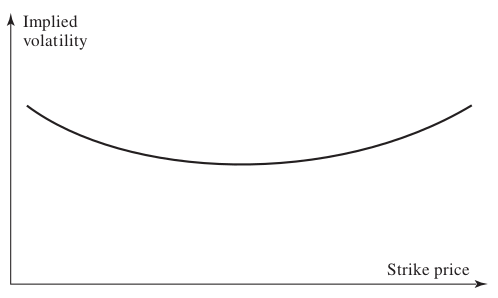
\includegraphics{./images/smile_cambial.png}
\caption{\label{fig:smile-cambial}Smile típico de um mercado cambial.}
\end{figure}

Caso a distribuição dos preços do ativo subjacente, neste caso uma taxa
de câmbio fosse perfeitamente log-normal como no modelo B\&S, o smile
não teria esta curvatura. Desta forma podemos afirmar que o mercado, ao
precificar as opções, acredita que a distribuição deste ativo possui
caudas com maior densidade que supõe a log-normal, existem maiores
probabilidades de retornos muito baixos ou muito altos.

\subsection{\texorpdfstring{Mercados de
\emph{equities}}{Mercados de equities}}\label{mercados-de-equities}

Nos mercados de \emph{equities}, ações, índices de ações e ETFs, por
exemplo, o smile apresenta uma característica de assimetria (skew, em
inglês) negativa. A asa esquerda (parte onde as puts estão fora do
dinheiro) apresenta valores de volatilidade implícita muito maiores que
suas contrapartes no lado das calls. Este comportamento reflete a
percepção de mercado de uma maior probabilidade de grandes perdas nas
ações que altos ganhos, gerando portanto, uma distribuição de preços
assimétrica. Como existe uma maior probabilidade de perdas extremas, o
seguro para estas, ou seja, uma put é relativamente mais cara que uma
call.

\begin{figure}
\centering
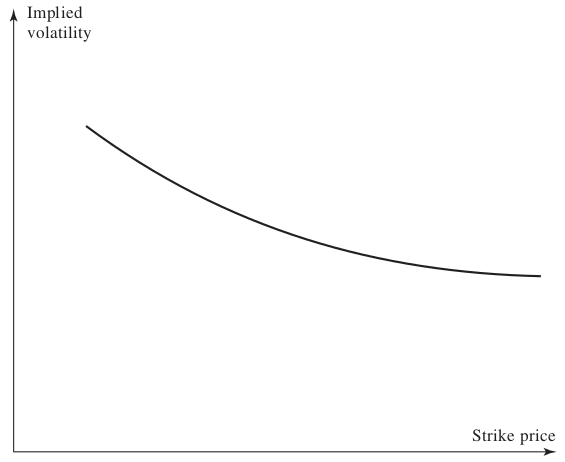
\includegraphics{./images/smile_equities.png}
\caption{\label{fig:smile-equities}Smile típico de uma ação ou índice de
ações.}
\end{figure}

\section{Smile como forma de precificação}\label{smileprecificacao}

Analisando a equação de B\&S com a parametrização para \(d1\) e \(d2\)
dada no início deste artigo é possível verificar que existe uma relação
direta entre volatilidade implícita e preço de uma opção, seja esta uma
call ou put.

Como \(d1\) é estritamente crescente em \(\theta\) e \(d2\) é
estritamente decrescente e ao mesmo tempo o preço de uma opção é
crescente em d1 e decrescente em d2, logo, temos uma relação direta
entre o preço de uma opção e sua volatilidade implícita para uma dada
maturidade. Em outras palavras, em um smile, tudo o mais constante,
quanto maior a volatilidade implícita maior o preço da opção naquele
\emph{strike}.

Outra forma de verificar esta relação é perceber que a grega Vega, que é
calculada da mesma forma para calls e puts, é sempre positiva. Ou seja,
um aumento no valor da volatiliade sempre leva a elevações no preço de
uma opção.

Desta forma é normal entre os praticantes de mercado fazer a
precificação de opções em termos de ``pontos de volatilidade'' e não em
valores monetários propriamente ditos. Isto porque o modelo B\&S, apesar
de não ser o modelo correto (nenhum é) para a precificação de opções, é
conhecido e de fácil entendimento para todos. Então todos os praticantes
podem fazer suas cotações em termos de volatilidades implícitas, que são
extraídas de opções baunilhas com o modelo B\&S, e somente na hora de
fechar um negócio e liquidar o pagamento, o preço efetivo a ser pago é
acordado entre as partes.

\section{Estrutura a termo}\label{estrutura-a-termo}

O mercado precifica a volatilidade implícita de forma que esta dependa
também do tempo até expiração, bem como do preço de exercício, agregando
uma segunda dimensão ao smile e transformando-o na famigerada
\textbf{superfície de volatilidade implícita}.

A volatilidade implícita tende a ser uma função crescente da maturidade
quando as volatilidades de curto prazo são historicamente baixas e
função decrescente da maturidade quando as volatilidades de curto prazo
são historicamente altas. Isso porque existe uma expectativa de reversão
a uma média de longo prazo embutida na volatilidade. Esta característica
é explorada explicitamente por alguns modelos de volatilidade, como em
\citet{Heston1993}.

As superfícies de volatilidade combinam smiles com a estrutura a termo
de volatilidade para tabular valores apropriados para precificar uma
opção com qualquer preço de exercício e prazo de expiração.

Da mesma forma como a curva de juros em um dado momento é uma descrição
concisa dos preços dos títulos negociados naquele mercado, assim, para
um ativo subjacente em particular em determinado momento, a superfície
de volatilidade implícita fornece uma descrição resumida de seu mercado
de opções. Considerando que os rendimentos dos títulos são diferenciados
pelo seu tempo até o vencimento, as opções são diferenciadas por seu
tempo até a expiração e o \emph{strike}, logo requerem uma superfície ao
invés de uma curva.

A figura \ref{fig:superficie} demonstra uma superfície de volatilidade
implícita do \texttt{SPX} em 15/09/2005, conforme apresentado em
\citet{Gatheral2011}.

\begin{figure}
\centering
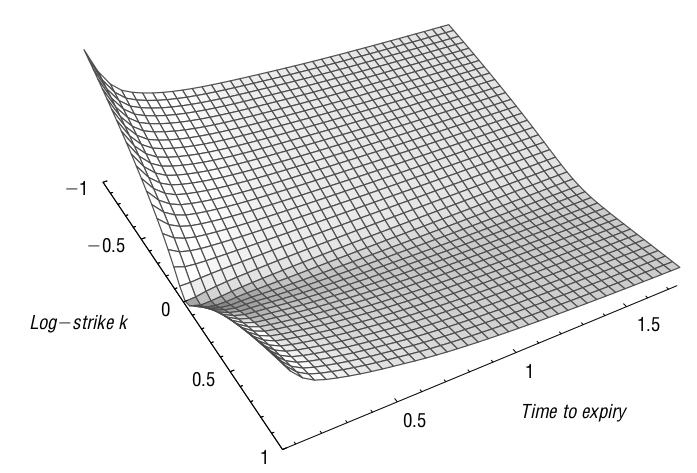
\includegraphics{./images/spx_vol_surface.png}
\caption{\label{fig:superficie}Superfície de volatilidade implícita.}
\end{figure}

\hypertarget{arbestatica}{\section{Arbitragem
estática}\label{arbestatica}}

Antes de definir o que é arbitragem estática que pode estar presente em
uma superfície de volatilidade (ou na superfície de preço de opções),
vamos partir para a intuição por trás desta definição.

O princípio de ausência de arbitragem é dominante na teoria financeira.
Este princípio nos informa que não deve existir lucro sem que se incorra
em algum tipo de risco, o lucro sempre é a remuneração do investidor que
aceitou carregar alguma forma de risco durante o investimento. Portanto,
não devem existir perfis de lucro acima da taxa livre de risco
(\emph{payoffs} positivos) com probabilidade de 100\%.

Primeiro consideramos uma trava de alta com opções do tipo call.
Excluindo-se os custos de transação, esta operação sempre oferece um
retorno positivo ou zero, conforme a figura \ref{fig:trava-alta}. Por
mais que esta estratégia esteja montada fora do dinheiro, sempre existe
uma possibilidade de ela ter lucro, \(S_T>K\) e portanto seu preço deve
ser sempre maior que zero.

\begin{figure}
\centering
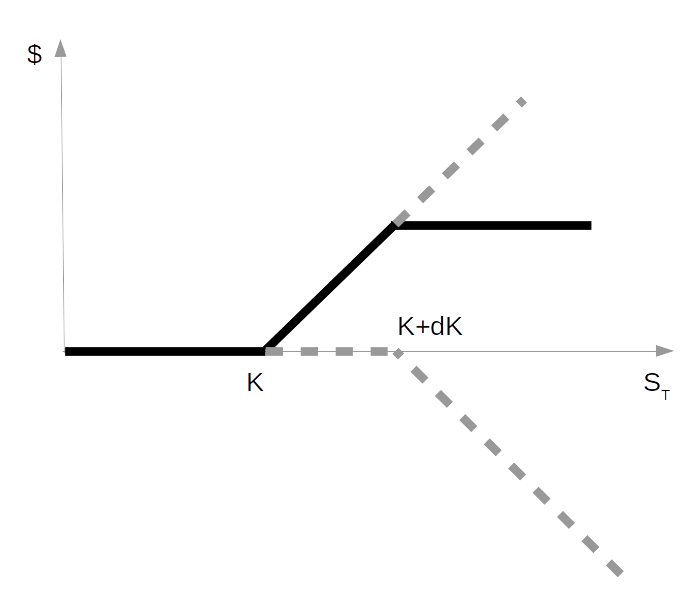
\includegraphics{./images/trava_alta.png}
\caption{\label{fig:trava-alta}Perfil de lucro de uma trava de alta.}
\end{figure}

É claro que quanto mais ITM estejam as opções, maior seu preço e quanto
mais fora do dinheiro menor será seu valor até o limite inferior zero.
Se levarmos a diferença entre os \emph{strikes}, \(dK\) a zero temos
que:

\begin{equation}
\frac{\partial C}{\partial K}\leq 0
\end{equation}

Este é o limite de arbitragem para travas de alta ou, mais conhecido
pelo termo em inglês \emph{call spread no-arbitrage} e impõe que os
preços das calls devem ser uma função descrescente no \emph{strike}. De
forma equivalente e através da \protect\hyperlink{putcalparity}{paridade
compra-venda} este limite de arbitragem para as puts é:

\begin{equation}
\frac{\partial P}{\partial K}\geq 0
\end{equation}

\subsection{Arbitragem de borboleta}\label{arbitragem-de-borboleta}

Também deve ser imposta uma restrição na segunda derivada do preço das
opções em relação ao \emph{strike}, e esta é conhecida como limite de
arbitragem para borboletas. Vejamos porquê.

Considere uma estratégia do tipo borboleta, onde se compra uma quantia
de calls no \emph{strike} \(K-dK\), vende-se duas vezes esta quantia em
\(K\) e compra-se novamente um lote em \(K+dK\), o perfil de lucro desta
operação no vencimento está representado na figura \ref{fig:borboleta}.

\begin{figure}
\centering
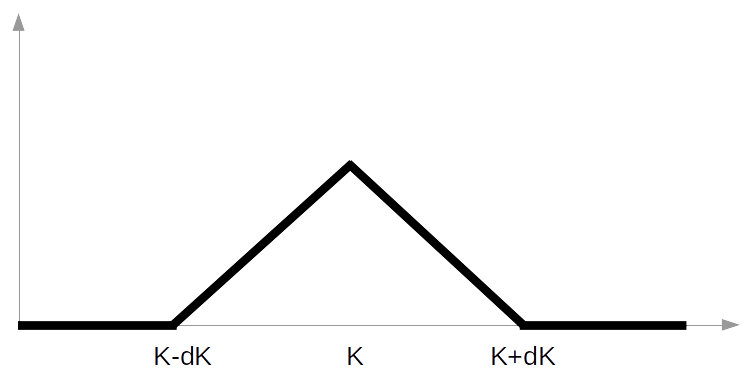
\includegraphics{./images/borboleta.png}
\caption{\label{fig:borboleta}Borboleta realizada com calls.}
\end{figure}

Seguindo a mesma linha de raciocínio anterior, como o \emph{payoff} da
borboleta é sempre não negativo também deve ser o seu valor para
qualquer período anterior a expiração. Se denotarmos \(\pi_B\) o valor
da borboleta, então \(\pi_B\geq0\).

Agora imagine que escalamos a estratégia de forma que um lote de compras
(na venda são dois lotes) seja de tamanho \(1/dK^2\), o valor para a
montagem desta operação deve ser, portanto:

\begin{equation}
\pi_B=\frac{C(K-dK)-2C(K)+C(K+dK)}{dK^2}
\end{equation}

E se levarmos ao limite em que \(dK\rightarrow 0\), a equação acima
torna-se justamente a segunda derivada do preço da call no \emph{strike}
\(K\).

\begin{equation}
\begin{aligned}
\frac{\partial^2 C(K)}{\partial K^2}=& \pi_B\\
\geq & 0
\end{aligned}
\label{eq:arbborboleta}
\end{equation}

Ou seja, os preços das calls são uma função \textbf{convexa} nos
\emph{strikes}. O mesmo raciocínio pode ser feito para uma borboleta com
puts e o resultado será equivalente, o preço das puts também deve ser
uma função convexa nos \emph{strikes}.

\subsection{Arbitragem de calendário}\label{arbitragem-de-calendario}

Passamos agora a analisar os limites de arbitragem na estrutura a termo
da superfície de volatilidade. A arbitragem de calendário normalmente é
expressa em termos de monotonicidade dos preços em relação ao período
para expiração. Ou seja, quanto maior o prazo de maturidade de uma opção
para um mesmo preço de exercício, maior deve ser seu valor.

É fácil de entender este limite com base nas probabilidades de
exercício. Como sabemos, em um
\protect\hyperlink{processos-estocasticos}{processo estocástico} do tipo
MBG a variância do processo cresce conforme a \textbf{raiz do tempo},
\(\sqrt{\tau}\). Quanto maior a variância do ativo subjacente, maior a
probabilidade deste alcançar um determinado preço, mais elevado ou não.
Assim, seja uma call ou put OTM quanto mais distante estiver seu prazo
de maturidade, maior a probabilidade de exercício e portanto, maior seu
valor.

Dado que a relação de \textbf{volatilidade total} implícita e preço de
uma opção também é direta e positiva, conforme demonstrado na Seção
\ref{smileprecificacao}, segue que a volatilidade total deve ser não
decrescente no tempo para expiração.

Esta relação pode ser expressa através da seguinte equação para uma call
precificada através de B\&S:

\begin{equation}
\frac{\partial C_{BS}(k, \theta(\tau))}{\partial \tau}=\partial_\theta C_{BS}\cdot\partial_\tau \theta \geq 0
\label{eq:arbcalendario}
\end{equation}

onde \(\partial_\theta C_{BS}\) é a derivada parcial do preço da call em
relação a volatilidade total implícita, que já demonstramos ser positiva
e \(\partial_\tau \theta\) é a derivada parcial da volatilidade total
implícita em relação ao tempo para maturidade que, portanto, deve ser
maior ou igual a zero para obedecer a restrição imposta ao preço da
call.

\section{Limites de inclinação}\label{limites-de-inclinacao}

Se mantivermos a volatilidade implícita constante para todos os
\emph{strikes}, os preços das calls no modelo B\&S devem ser
decrescentes. Por outro lado, para um \emph{strike} fixo, o preço de uma
call se eleva à medida que a volatilidade implícita aumenta. Suponha por
um momento que a volatilidade implícita varia com o \emph{strike} como é
o caso nos smiles. À medida que o \emph{strike} aumenta, se a
volatilidade implícita aumentar muito rapidamente, seu efeito sobre o
preço da call pode mais que compensar o declínio no preço devido a
elevação do preço de exercício e, assim, levar a um aumento líquido no
preço da opção. Isso violaria o requisito de que
\(\partial C /\partial K \leq 0\) e, portanto, leva a um limite superior
na taxa em que a volatilidade implícita pode aumentar com o strike.

Novamente, o mesmo raciocínio pode ser imposto para o lado das puts. A
volatilidade implícita não pode se elevar tão rapidamente quando os
\emph{strikes} se reduzem de forma que uma put de \emph{strike} menor
tenha valor mais elevado que outra que esteja mais próxima do dinheiro.

Finalmente, um sumário dos limites impostos a uma superfície de preços
de opções (calls no caso apresentado), que implicam em limites para a
superfície de volatilidade é apresentado abaixo\footnote{Retirado de
  \citet{Aurell2014}, p.~25.}:

\begin{enumerate}
\def\labelenumi{\arabic{enumi}.}
\tightlist
\item
  \(\partial_\tau C \geq 0\)
\item
  \(\lim\limits_{K\rightarrow\infty}C(K, \tau)=0\)
\item
  \(\lim\limits_{K\rightarrow-\infty}C(K, \tau)+K=a, \quad a \in \mathbb R\)
\item
  \(C(K, \tau)\) é convexa em \(K\)
\item
  \(C(K, \tau)\) é não-negativa
\end{enumerate}

\hypertarget{rnd}{\section{Distribuição implícita}\label{rnd}}

O modelo B\&S é baseado na suposição que o ativo subjacente segue uma
distribuição log-normal em seus preços. Caso esta suposição fosse de
fato realizada no mercado, o smile de volatilidade seria uma reta
completamente horizontal, não haveria variação na volatilidade implícita
conforme o preço de exercício. Entretanto, esta não é a realidade dos
smiles e podemos fazer a pergunta inversa portanto, qual a distribuição
neutra ao risco que está implícita no smile de volatilidade?

Certamente não é uma log-normal. Na verdade, a densidade da distribuição
que está implícita em um smile nada mais é que a convexidade deste
smile, ou seja, sua segunda derivada em relação ao \emph{strike}. Esta
distribuição implícita também é por vezes chamada de RND \emph{(risk
neutral density)} e é muito útil para fazer a precificação de outras
opções que não são observadas no smile ou extrair probabilidades de
ocorrência de eventos precificadas pelo mercado.

Pode-se obter este resultado a partir da definição do valor de uma call
e é conhecido como a fórmula de \citet{Breeden1978}. O valor de uma call
é o valor esperado do \emph{payoff} terminal desta call ponderado pela
densidade neutra ao risco do subjacente. Ou seja:

\begin{equation}
C(S, t)=e^{-r\tau}\int\limits_{0}^\infty p(S,t,S_T,T)\max\{S_T-K, 0\}dS_T
\end{equation}

onde \(p(\cdot)\) é a densidade neutra ao risco e estamos supondo uma
taxa de juros livre de risco constante durante o período de vida da
opção. Como o \emph{payoff} da call é não linear, sendo zero para
qualquer valor de \(S_T \leq K\) e igual a \(S_T-K\) quando \(S_T > K\),
podemos escrever esta equação como:

\begin{equation}
C(S, t)=e^{-r\tau}\int\limits_{K}^\infty p(S,t,S_T,T)(S_T-K)dS_T
\end{equation}

que pode ser rearranjada, com alguma simplificação na notação, da
seguinte forma.

\begin{equation}
\begin{aligned}
\frac{\partial C}{\partial K}=& -e^{-r\tau}\int\limits_{K}^\infty p(S_T)dS_T\\
e^{r\tau}\frac{\partial C}{\partial K}=& \int\limits_{-\infty}^K p(S_T)dS_T\\
e^{r\tau}\frac{\partial^2 C}{\partial K^2}=& \ p(K)\\
\frac{\partial^2 C_B}{\partial K^2}=& \ p(K)
\end{aligned}
\label{eq:distimplicita}
\end{equation}

Onde usou-se a notação \(C_B\) para denotar a formulação de Black para o
preço de uma call. Ou seja, a segunda derivada em relação ao strike do
preço não descontado de uma call é a distribuição neutra ao risco do
ativo subjacente, e é válida para todos preços de exercício.

Portanto, se desejarmos saber qual a distribuição de probabilidades de
preços do ativo subjacente em uma data futura que possua vencimento de
opções, basta encontrarmos a convexidade do smile dos preços
\emph{forward} daquele vencimento\footnote{Simples em teoria, muito mais
  complicado na prática, com diversos problemas para a extrapolação do
  smile para \emph{strikes} extremos.}.

\section{Conclusão}\label{conclusao}

O modelo de Black-Scholes-Merton, pode ser considerado a pedra
fundamental para a precifição de opções. Entretanto, este modelo
apresenta uma séries de limitações que fazem com que os praticantes de
mercado utilizem outras técnicas neste mercado. Uma destas é o uso do
smile de volatilidade e sua interpretação como forma de precificar
opções e extrair informações implícitas nos preços.

A assimetria do smile e suas asas informam que as distribuições de
probabilidades para o ativo subjacente não são exatamente log-normais, e
podem apresentar discrepâncias significativas, especialmente nas caudas
da distribuição que muito interessam a gestão de risco, por exemplo.

Este foi um artigo denso, porém com vários conceitos importantes para a
compreensão do comportamento da superfície de volatilidade. A estrutura
a termo também é existente na volatilidade implícita e está limitada
pela ausência de arbitragem do tipo calendário. O smile de volatilidade,
que é uma fatia da superfície com prazo de expiração constante, possui
suas próprias limitações de forma, com a ausência de arbitragem do tipo
borboleta e limitações quanto a inclinação.

Por fim, foi demonstrado como a convexidade do smile de preços fornece a
distribuição implícita para os preços do ativo subjacente para a data de
expiração das opções.

\hypertarget{superficies}{\chapter{Superfícies de
volatilidade}\label{superficies}}

Já mostramos em artigos anteriores,
\protect\hyperlink{processos-estocasticos}{processos estocásticos em
finanças}, o \protect\hyperlink{bsm}{modelo de Black\&Scholes} e, como
na realidade dos mercados surgem os \protect\hyperlink{smile}{smiles de
volatilidade}, uma anomalia não prevista por B\&S. Dado que este modelo
não pode explicar o surgimento do smile de volatilidade e tampouco sua
superfície, o estudo da volatilidade implícita tornou-se uma preocupação
central nas finanças. Diversos modelos foram propostos ao longo dos
anos, e ainda o são, para buscar conciliar a presença do smile de
volatilidade e a natureza estocástica da precificação do ativo
subjacente.

Apresentaremos alguns poucos destes modelos.

\section{Modelos estocásticos}\label{modelos-estocasticos}

Volatilidade estocástica apresenta a noção que a volatilidade
instantânea do ativo subjacente também é, por si só, um processo
estocástico que pode ser correlacionado com o processo de formação do
preço do ativo. O resultado destes modelo é um procedimento livre de
arbitragem para a interpolação dos dados de mercado a superfície de
volatilidade.

\subsection{Heston}\label{heston}

O modelo de Heston, baseado no trabalho de \citet{Heston1993}, assume
que o quadrado da volatilidade segue uma equação diferencial estocástica
- EDE - do tipo Cox-Ingersoll-Ross - CIR, a qual apresenta
características desejáveis do ponto de vista da variância. Abaixo estão
as três equações que definem um modelo de Heston:

\begin{equation}
\begin{aligned}
dS_t=&\mu S_t dt + \sqrt{v_t}S_t dW_1\\
dv_t=&-\lambda(v_t-\bar v)dt+\eta\sqrt{v_t}dW_2\\
d\left\langle W_1, W_2 \right\rangle=&\rho dt
\end{aligned}
\label{eq:heston}
\end{equation}

onde \(v_t\) é a variância estocástica, \(\lambda\) é o parâmetro que
define a velocidade de convergência da volatilidade para seu valor de
longo prazo \(\bar v\), \(\eta\) é a famigerada \textbf{volatilidade da
volatilidade} e a notação \(d\left\langle W_1, W_2 \right\rangle\)
indica a covariação entre os movimentos Brownianos padrões \(dW_1\) e
\(dW_2\).

Esta modelagem apresenta uma característica desejável, e até certo
ponto, intuitiva para a volatilidade, o retorno a uma média de longo
prazo. Empiricamente observamos regimes distintos de volatilidade para
os ativos financeiros, em alguns momentos a volatilidade está
anormalmente baixa ou durante momentos de estresse no mercado,
incrivelmente alta. Porém não faria sentido um modelo onde a volatiliade
pudesse estacionar permanentemente no limite inferior ou então divergir
para infinito. O modelo de Heston garante que, mesmo sendo estocástica,
a volatilidade não é atraída para estes extremos.

Os preços das calls e puts européias possuem fórmula fechada para seu
cômputo através da
\href{https://en.wikipedia.org/wiki/Fourier_transform}{transformada de
Fourier}, como apresentado no artigo original. A complexidade destas
equações e do método para sua resolução está fora do escopo deste blog,
entretanto o leitor aficcionado pode encontrar uma demonstração da forma
de resolução em \citet{Gatheral2011}.

Basta-nos saber que em um \emph{framework} geral de precificação de
derivativos, o preço de uma call não descontada (preço de Black) pode
ser escrita da seguinte forma:

\begin{equation}
C_B(x, v, \tau)=K\left[e^xP_1(x, v, \tau)-P_0(x, v, \tau)\right]
\label{eq:callgeral}
\end{equation}

onde \(x:=\ln K/F_t\). \(P_1\) e \(P_0\) são duas probabilidades na
medida neutra ao risco, \(\mathbb Q\). Enquanto \(e^xP_1\) informa o
valor esperado do ativo no vencimento dado que a opção está no dinheiro,
\(P_0\) representa a probabilidade de ficar dentro do dinheiro na data
de expiração.

As probabilidades \(P_j\), \(j = 0, 1\) podem ser calculadas através da
seguinte equação:

\begin{equation}
P_j(x, v, \tau)=\frac{1}{2}+\frac{1}{\pi}\int\limits_0^\infty
    Re\left\lbrace\frac{exp\{C_j(u, \tau)\bar v + D_j(u, \tau)v + iux\}}{iu}\right\rbrace du
\label{eq:pj}
\end{equation}

onde \(i\) representa o número imaginário \(\sqrt{-1}\) e
\(Re\{\cdot\}\) é apenas a parte real de seu argumento.

Primeiramente vamos definir algumas variáveis auxiliares:

\[\alpha_j=-\frac{u^2}{2}-\frac{iu}{2}+jiu\]

\[\beta_j=\lambda-j\rho\eta-\rho\eta i u\]

\[\gamma=\frac{\eta^2}{2}\]

\[r_{\pm}=\frac{\beta_j\pm\sqrt{\beta^2-4\alpha\gamma}}{2\gamma}=\frac{\beta\pm d}{\eta^2}\]

\[d=\sqrt{\beta^2-4\alpha\gamma}\]

\[g=\frac{r_-}{r_+}\]

Então:

\[C_j(u, \tau)=\lambda\left\lbrace  r_-\tau-\frac{2}{\eta^2}\ln\left(\frac{1-ge^{-d\tau}}{1-g}\right) \right\rbrace
\label{eq:cj}\]

\[D_j(u, \tau)=r_-\frac{1-e^{-d\tau}}{1-ge^{-d\tau}}
\label{eq:dj}\]

\subsection{SABR}\label{sabr}

Este modelo foi apresentado por \citet{Hagan2002} e assume que o preço
\emph{forward}, \(F_t\) do ativo subjacente e sua volatilidade
instantânea, \(\alpha_t\), seguem as seguintes EDEs:

\[
\begin{aligned}
dF_t=&\alpha_tF_t^\beta dW_1\\
d\alpha_t=&\nu\alpha_t dW_2\\
d\left\langle W_1, W_2 \right\rangle =&\rho dt
\end{aligned}
\label{eq:sabr}
\]

onde \(\nu > 0\) é a volatilidade da volatilidade e \(\beta > 0\) é
conhecido como o coeficiente de alavancagem.

A interpretação financeira se dá pela seguinte maneira: \(\alpha_t\)
determina o nível geral de volatilidade do \emph{forward} no dinheiro,
\(\beta\) mede a assimetria do smile sendo as duas escolhas
particulares: \(\beta = 1\) correspondendo ao modelo log-normal sem
smile e \(\beta = 0\) correspondendo ao modelo normal com um smile
irrealista, \(\rho\) também controla a inclinação do smile, quando
\(\rho < 0\) uma inclinação negativa típica de \emph{equities} surge e
com a opção \(\rho = 0\) produzindo um smile de volatilidade simétrico,
por fim, \(\nu\) é uma medida de convexidade. Também é possível
verificar que a volatilidade estocástica, \(\alpha_t\) segue uma
distribuição log-normal.

Comparado com outros modelos de volatilidade estocástica, o SABR é um
dos mais simples e possui aproximações analíticas para o cálculo do
preço de opções Europeias. Ele pode ser utilizado para ajustar um smile
observado no mercado de forma acurada, entretanto, para ajustar uma
superfície completa este modelo sofre com algumas restrições.

\subsection{Bates}\label{bates}

Em modelos de difusão como B\&S e mesmo Heston, o processo de formação
de preço do ativo se comporta como um movimento browniano e a
probabilidade de que este preço se mova bruscamente em um curto período
de tempo é muito pequena. Assim, em tais modelos, os preços das opções
OTM mais curtas são muito inferiores ao que se observa nos mercados
reais.

Para endereçar esta deficiência, \citet{Bates1996} amplia o modelo de
Heston incluindo saltos no processo de preço do ativo subjacente. Estes
modelos, com a inclusão de saltos aleatórios na dinâmica de preços são
conhecidos como \emph{Jump-Diffusion}. A dinâmica é especificada pelas
seguintes equações:

\begin{equation}
\begin{aligned}
dS_t=&\mu S_tdt+\sqrt{v_t}S_tdW_1(t)+J_t S_t dN_t\\
dv_t=&-\lambda(v_t-\bar v)dt+\eta\sqrt{v_t}dW_2(t)\\
d\left\langle W_1, W_2 \right\rangle =&\rho dt
\end{aligned}
\label{eq:bates}
\end{equation}

Muito semelhante, portanto ao modelo de Heston nas equações
\eqref{eq:heston}, com a diferença da inclusão de um processo de Poisson,
\(dN_t\) com intensidade \(\theta\) indicando a probabilidade
instantânea de um salto de tamanho unitário. \(J_t\) é o tamanho do
salto aleatório e seu logaritmo segue uma distribuição gaussiana:

\begin{equation}
\ln{(1+J)}\sim N\left(\ln(1+\beta)-\frac{1}{2}\alpha^2\,\, ,\,\,\alpha^2\right)
\label{eq:jt}
\end{equation}

Este modelo possui fórmulas fechadas para os preços de calls e puts,
novamente utilizando-se o método da transformada de Fourier, que podem
ser encontrados utilizando o método de \citet{Duffie2000}.

\subsection{Volatilidade local}\label{volatilidade-local}

Conforme visto na \protect\hyperlink{rnd}{seção anterior} sobre o smile
de volatilidade, é possível a partir das volatilidades implícitas obter
a distribuição neutra ao risco do preço terminal do ativo subjacente. O
pesquisador e profissional de mercado Bruno Dupire em seu artigo,
\citet{Dupire1994}, fez então o seguinte questionamento: dada uma
distribuição implícita, existe apenas um processo de difusão\footnote{Processo
  de difusão é a solução de uma equação diferencial estocástica com
  propriedades de Markov. O Movimento Browniano é um exemplo.} que seja
consistente com esta distribuição? A resposta obtida foi sim, e deste
processo surge a função de volatilidade local, \(\sigma_L(S, t)\), por
vezes também conhecida como função de volatilidade implícita.

A equação de Dupire é apresentada abaixo:

\[\frac{\partial C_B}{\partial \tau}=\frac{1}{2}\sigma_L^2K^2\frac{\partial^2C_B}{\partial K^2}
\label{eq:dupire}\]

da qual todos os termos podem ser obtidos a partir dos dados de mercado
de uma superfície de volatilidade, com exceção é claro, da função de
volatilidade local \(\sigma_L\) que poderá ser calculada. Esta equação
pode ser vista como a definição da função de volatiliade local
independente do processo que governa a evolução da volatilidade (um
processo estocástico, por exemplo).

Uma forma de interpretar a volatilidade, ou mais precisamente a
variância local, é na forma de valor esperado dentro da medida neutra ao
risco. Resultado devido a trabalho de \citet{Derman1998}, onde a equação
de Dupire pode ser reescrita da seguinte forma:

\[\frac{\partial C_B}{\partial \tau}=\mathbb E\left[v_T|S_T=K\right]\frac{1}{2}K^2\frac{\partial^2C_B}{\partial K^2}
\label{eq:derman}\]

Ou seja, a variância local é a expectativa neutra ao risco da variância
instantânea condicionada ao preço terminal do ativo, \(S_T\) ser igual
ao preço de exercício \(K\).

Uma das formas mais praticadas para a implementação de uma superfície de
volatilidade local é através de árvores binomiais conforme apresentado
por \citet{Derman1994}.

\section{Modelos paramétricos}\label{modelos-parametricos}

Diversas representações paramétricas já foram apresentadas para a
superfície de volatilidade. Neste tipo de modelo uma função não-linear,
dependente de um conjunto de parâmetros é especificada e, a partir dos
dados observados no mercado, a parametrização é encontrada através da
minimização de alguma função objetivo, método conhecido como
\textbf{calibração}.

\subsection{SVI}\label{sec:svi}

A parametrização da do tipo SVI \emph{(Stochastic Volatility Inspired)}
para o \emph{smile} foi introduzida por \citet{Gatheral2004} e é
motivada pelo comportamento assintótico para \emph{strikes} extremos. É
baseada no \emph{smile} gerado por um modelo de \citet{Heston1993}. Sua
parametrização é dada em termos de \emph{forward log-moneyness} conforme
apresentado \protect\hyperlink{smile}{anteriormente},
\(k=\ln(K/S)-r\tau=\ln(K/F)\), por:

\begin{equation}
w(k) = a + b\left(\rho(k-m)+\sqrt{(k-m)^2 + \sigma^2}\right)
\label{eq:rawsvi}
\end{equation}

onde \(w\) é a variância total e o conjunto de parâmetros
\(\chi_R = \{a, b, \rho, m, \sigma\}\) definem a forma deste
\emph{smile} que é conhecido como parametrização \textbf{\emph{raw}} do
SVI. Os limites destes parâmetros são tais que: \(a \in \mathbb R\),
\(b \geq 0\), \(|\rho| < 1\), \(m \in \mathbb R\), \(\sigma > 0\), e a
condição ``óbivia'' segundo \citet{Gatheral2014},
\(a+b \sigma\sqrt{1 − \rho^2} \geq 0\), que garante
\(w(k; \chi_R) \geq 0\) para todo \(k \in \mathbb R\). Alterações nestes
parâmetros têm os seguintes efeitos:

\begin{itemize}
\tightlist
\item
  Aumentar \(a\) eleva o nível geral de variância, um deslocamento
  vertical do \emph{smile}
\item
  Aumentar \(b\) aumenta as inclinações das asas, comprimindo o
  \emph{smile}
\item
  Aumentar \(\rho\) provoca uma rotação no sentido anti-horário
\item
  Aumentar \(m\) desloca o smile para a direita
\item
  Aumentar \(\sigma\) reduz a curvatura no dinheiro (ATM) do
  \emph{smile}
\end{itemize}



\begin{figure}
\centering
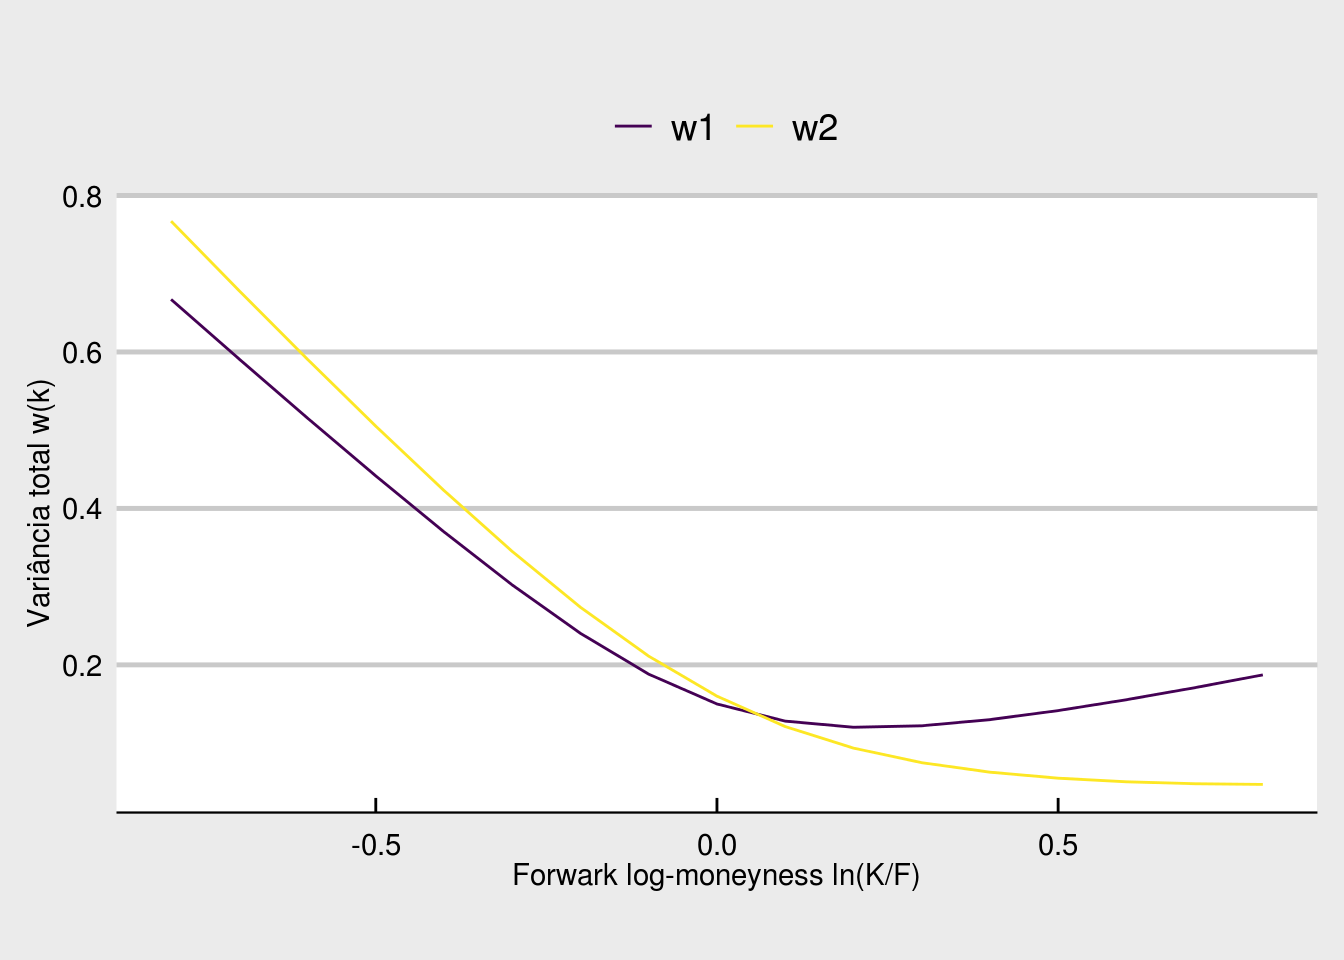
\includegraphics{051-superficies-de-volatilidade_files/figure-latex/svi-1.pdf}
\caption{\label{fig:svi}Duas parametrizações hipotéticas para a SVI.}
\end{figure}

A figura \ref{fig:svi} acima apresenta duas parametrizações hipotéticas
para o modelo. A variância total \(w_1\) tem como conjunto de
parâmetros, \(\chi = \{0, 0.5, -0.6, 0, 0.3\}\) e poderia representar um
\emph{smile} de taxas de câmbio por exemplo. Enquanto que o modelo
\(w_2\) conta com \(\chi = \{-0.04, 0.5, -0.9, 0, 0.4\}\) e se ajusta
melhor ao mercado de \emph{equities}.

Existem outras duas parametrizações para o SVI, a natural e a
\emph{jump-wings} que podem ser conferidas no artigo de
\citet{Gatheral2014} e serão abordadas em outro artigo a ser publicado
futuramente pelo \href{https://clubedefinancas.com.br}{CF}.

O SVI tem muitas vantagens, como o baixo tempo computacional, a
variância implícita se comporta linearmente nos extremos, conforme
prescrito pela fórmula do momento de \citet{Lee2004}, e boa aproximação
de volatilidades implícitas para \emph{strikes} muito dentro ou fora do
dinheiro. O ajuste do SVI para os mercados de \emph{equities} é muito
melhor do que para outros mercados.

\section{Modelos não-paramétricos}\label{modelos-nao-parametricos}

Se violações de arbitragem na estimativa da superfície não representam
um problema de interesse particular, virtualmente qualquer método
não-paramétrico pode ser aplicado a dados de volatilidade implícita. Uma
escolha específica deve ser feita a partir de considerações práticas.

\subsection{Interpolação e suavização
spline}\label{interpolacao-e-suavizacao-spline}

As seguintes splines\footnote{\href{https://en.wikipedia.org/wiki/Spline_interpolation}{Spline}}
podem ser empregadas para interpolar \emph{smiles} de volatilidade:

\begin{itemize}
\tightlist
\item
  Spline cúbica
\item
  B-spline cúbica
\end{itemize}

No caso da spline cúbica, esta é uma função polinomial de grau 3
definida em cada subintervalo demarcados pelos pontos de controle, no
caso de interpolação são todos nós. Uma spline cúbica é uma função
contínua, suave e diferenciável até a segunda ordem.

Uma B-spline\footnote{\href{https://en.wikipedia.org/wiki/B-spline}{B-Spline}},
ou \emph{basis-spline} é uma função básica para funções spline de mesma
ordem, o que significa que todas as funções spline possíveis podem ser
construídas a partir de uma combinação linear de B-splines. Estas podem
ser preferidas às splines cúbicas, devido à sua robustez a dados ruins e
à capacidade de preservar a monotonicidade e a convexidade.

Praticamente qualquer linguagem de programação e até mesmo o
Excel\footnote{\href{https://www.business-spreadsheets.com/forum.asp?t=120}{Cubic
  Spline Function in VBA}} possui funções pré-programadas para
implementar interpolações spline, sendo um método de fácil aplicação.
Entretanto, estas técnicas de interpolação não são específicas para
superfícies de volatilidade e, portanto, não garantem que a superfície
interpolada seja livre de oportunidades de arbitragem, mesmo que os
dados apresentados o sejam.

\subsection{Algoritmos livres de
arbitragem}\label{algoritmos-livres-de-arbitragem}

Considerando as limitações das interpolações com relação a presença de
arbitragem na superfície gerada, vários artigos propõe algoritmos de
interpolação que garantem que oportunidades de
\protect\hyperlink{arbestatica}{arbitragem estática} não se apresentem,
como em \citet{Kahale2004} e \citet{Wang2004}.

Em comum, estes algoritmos possuem como requisito que os dados a serem
interpolados sejam livres de arbitragem desde o início, o que nem sempre
pode ser obtido. \citet{Kahale2004}, por exemplo, propõe um procedimento
de interpolação baseado em polinômios convexos por partes que simulam a
fórmula de B\&S. O resultado da função de preço de calls é livre de
arbitragem e, portanto, também a volatilidade implícita calculada a
partir dela. Em uma segunda etapa, a variância total implícita é
interpolada linearmente ao longo dos \emph{strikes}.

A abordagem de \citet{Fengler2012} é baseada na suavização dos preços
das opções por spline cúbica, e não em interpolação. Desta forma, os
dados de entrada não precisam ser livres de arbitragem. Restrições
especificamente adicionadas ao problema de minimização, a fim de
garantir que não haja arbitragem, são impostos ao algoritmo spline. Uma
possível desvantagem dessa abordagem é o fato de que a função de preço
calls é aproximada por polinômios. Isso pode se mostrar desvantajoso,
especialmente se extrapolação for necessária, já que a função de
precificação certamente não é um polinômio. A escolha de uma grade
suficientemente densa nos \emph{strikes} pode minimizar este problema.

\section{Extrapolação do smile}\label{extrapolacao-do-smile}

É argumentado em \citet{Benaim2008} que que um método de extrapolação
deve resultar em preços livres de arbitragem para as opções europeias
(baunilha), ou seja, os preços das opções devem ser funções decrescentes
(crescentes) para calls (puts), convexas com relação ao \emph{strike}, e
permanecer dentro de certos limites de inclinação. Além disso, o método
de extrapolação deve idealmente ter as seguintes propriedades:

\begin{enumerate}
\def\labelenumi{\arabic{enumi}.}
\tightlist
\item
  Deve precificar corretamente todas as opções baunilha observadas
\item
  A densidade da distribuição implícita e os preços das opções baunilha
  devem ser fáceis de calcular
\item
  O método não deve gerar caudas irrealistas e, se possível, deve
  permitir controlá-las
\item
  Deve ser robusto e flexível o suficiente para ser usado com uma ampla
  variedade de superfícies de volatilidade implícita
\item
  Deve ser fácil e rápido inicializar para um determinado \emph{smile}
\end{enumerate}

Uma das formas de extrapolação comumente utilizada é fazer a
interpolação dos dados dentro da área observada, por exemplo com splines
cúbicas, e então fazer a extrapolação na forma de uma linha reta, ou
seja, mantendo na região de extrapolação a mesma inclinação observada no
último ponto interpolado. Esta forma, segundo os autores não é adequada
pois insere uma descontinuidade na densidade e também gera caudas muito
curtas, de fato truncadas, a partir do ponto onde se inicia a
extrapolação.

É proposto um método de extrapolação através de fórmulas fechadas para a
asa esquerda (OTM puts) e direita (OTM call) do \emph{smile}. Estas
fórmulas têm as propriedades desejadas para \emph{strikes} extremos e
mantêm a convexidade dos preços. Suponha um intervalo de preços de
exercício os quais existem observações de mercado e portanto, é possível
fazer interpolação: \(K_-\leq K \leq K_+\), os valores das puts,
\(P(K)\), para \(K<K_-\) e das calls, \(C(K)\), para \(K>K_+\) são dados
por:

\begin{equation}
P(K)=K^\mu \exp\left(a_1+b_1K+c_1K^2\right)
\label{eq:pk}
\end{equation}

\begin{equation}
C(K)=K^{-\nu} \exp\left(a_2+\frac{b_2}{K}+\frac{c_2}{K^2}\right)
\label{eq:ck}
\end{equation}

onde se garante \(\lim\limits_{K\rightarrow 0} P(K)=0\) e
\(\lim\limits_{K\rightarrow \infty} C(K)=0\), fazendo \(\mu > 1\) e
\(\nu > 0\). Estes parâmetros também servem para controlar a massa de
probabilidade sob as caudas da distribuição.

As condições para ajustar o preço e suas duas primeiras derivadas em
\(K_-\) e \(K_+\) produz um conjunto de equações lineares para os
parâmetros \(a_1, b_1, c_1\) e \(a_2, b_2, c_2\), respectivamente.

\section{Conclusão}\label{conclusao-1}

Repassamos neste artigos, algumas das principais metodologias para a
construção da superfície de volatilidade implícita. Modelos de
volatilidade estocástica são capazes de gerar \emph{smiles} compatíveis
com aqueles observados nos mercados, sendo dependentes de técnicas de
calibração destes modelos. O modelo paramétrico SVI pode ser adequado
para mercado de \emph{equities}, entretanto, assim como acontece nas
técnicas de interpolação, restrições com relação aos parâmetros devem
ser impostas a fim de evitar o surgimento de oportunidades de arbitragem
estática. Por fim uma estratégia de como implementar a extrapolação do
\emph{smile} fora da região central foi apresentada.

\section{Referências}\label{referencias}

\hypertarget{calibracao}{\chapter{Métodos de
Calibração}\label{calibracao}}

Neste post iremos mostrar as diferenças existentes entre
``interpolação'', ``suavização'' e ``parametrização'' de superfícies de
volatilidade.

Como já apresentado em posts anteriores, existem diversas formas de
interpolar, extrapolar, parametrizar e calibrar smiles de volatilidade.
Exsitem vantagens e desvantagens para cada método.

\section{Calibração versus
Interpolação}\label{calibracao-versus-interpolacao}

Uma forma simples de gerar um smile de volatilidade a partir de dados
observados no mercado é a \textbf{interpolação} destes dados. Diversas
formas de interpolação existem, sendo talvez a mais conhecida a spline
cúbica. Não é a proposta deste artigo detalhar os procedimentos de
interpolação, restando saber que em tal procedimento é gerada uma função
contínua em partes (piecewise) que \textbf{passa} por todos os pontos
observados.

Uma interpolação força a passagem da função interpolada em todos os seus
pontos de referência, como se estivesse ligando os pontos em um desenho
a mão livre. Portanto, nestes pontos o erro da interpolação é zero por
definição, entretanto em pontos intermediários podem surgir erros,
inclusive aqueles que possibilitam a existência de arbitragem entre
strikes de um mesmo smile\footnote{Veja mais detalhes no Capítulo
  \protect\hyperlink{arbestatica}{Smile de Volatilidade}}.

Em contraposição a métodos de interpolação, podem ser derivados métodos
de suavização (smoothing) ou então a parametrização do smile de
volatilidade. Seja suavização, ou parametrização, estes métodos não
forçam a passagem da função que representa o smile pelos pontos de
mercado, mas buscam minimizar alguma função perda com relação aos
desvios em relação a estes pontos ao mesmo tempo em que buscam
``suavizar'' o smile, para que este não apresente variações bruscas
entre os strikes ou alterações de convexidade na curva de preços, que
não são condizentes com a teoria de precificação de derivativos.

Um método paramétrico, como o SVI, Heston, SABR ou Volatilidade Local,
busca ajustar às volatilidades implícitas observadas através dos preços
das opções sendo praticados no mercado uma determinada função, que
possui parâmetros em sua definição que por sua vez determinam a forma
desta função. Ao se ajustar os parâmetros, pode-se adequar a função para
ficar ``o mais próxima possível'' dos dados observados, sem
necessariamente, no entanto, passar por todos estes pontos.

A figura abaixo tenta mostrar as diferenças entre uma interpolação
spline cúbica, uma suavização e uma parametrização SVI. Enquanto que a
interpolação liga todos os pontos marcados, a suavização e a
parametrização não necessariamente passam sobre estes pontos mas
fornecem uma curva mais ``suave'', sem trocas de convexidade, o que gera
oportunidades de arbitragem e probabilidades negativas de ocorrência de
determinados preços para o ativo subjacente, que ferem os princípios de
precificação de opções. Os dados utilizados neste e nos próximos artigos
sobre superfícies de volatlidade foram obtidos do site
\href{http://www.ivolatility.com/doc/usa/IV_Raw_Delta_surface.csv}{ivolatility.com}
na forma de amostra gratuita fornecida livremente. O ativo subjacente é
o ETF
\href{https://www.ishares.com/us/products/239710/ishares-russell-2000-etf}{\texttt{IWM}}
para a data de 21/09/2017.

\begin{figure}
\centering
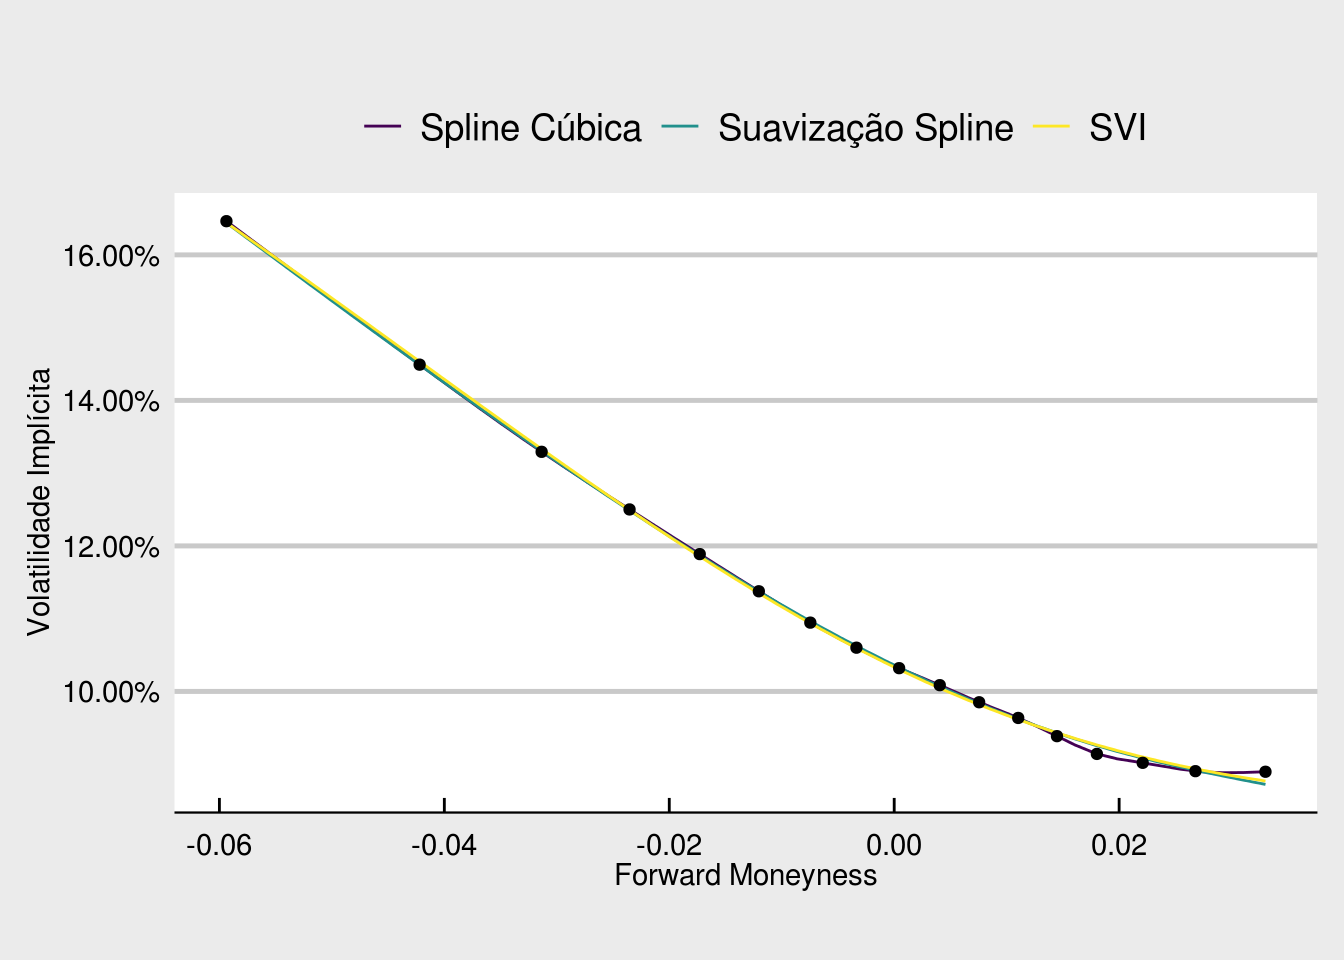
\includegraphics{06-metodos-calibracao_files/figure-latex/diferencas-1.pdf}
\caption{\label{fig:diferencas}Diferentes métodos de ajuste de dados a um
smile.}
\end{figure}

Pode-se verificar como os métodos SVI e a suavização não passam sobre
todos os pontos marcados, com a suavização tendo dificuldade com a
curvatura nos valores mais altos de \emph{moneyness} e a SVI possuindo
uma inclinação mais branda na asa esquerda do smile.

\section{Spline cúbica}\label{spline-cubica}

Este método é possivelmente um dos mais flexíveis e conhecidos de
interpolação de dados univariados existente, embora também exista sua
versão bi-dimensional. Uma spline nada mais é que ``uma curva definida
matematicamente por dois ou mais pontos de controle''\footnote{Definição
  retirada de \url{https://pt.wikipedia.org/wiki/Spline}}.

No caso da spline cúbica, esta é uma função polinomial de grau 3
definida em cada subintervalo demarcados pelos pontos de controle, no
caso de interpolação são todos nós. Ou seja, considere um segmento entre
dois pontos consecutivos \([c, d]\in S\) a spline é uma função cúbica
com seus parâmetros calculados pelo algoritmo de ajuste. Para o próximo
intervalo de pontos dentro do domínio da função, um novo polinômio de
grau 3 é ajustado, sendo que nos pontos de nós uma restrição de
igualdade entre as derivadas nos dois segmentos é aplicada para garantir
a suavidade da função interpolada como um todo.

Assim, uma spline cúbica é uma função contínua, suave e diferenciável
até a segunda ordem. Entretanto, suas derivadas, apesar de contínuas,
podem não ser suaves, especialmente aquela de segunda ordem que pode
apresentar pontos de ``ruptura''. Esta característica de uma spline
cúbica a torna pouco atrativa para a inferência de distribuições de
probabilidade a partir de dados de volatilidade ou mesmo dos preços de
opções.

\begin{figure}
\centering
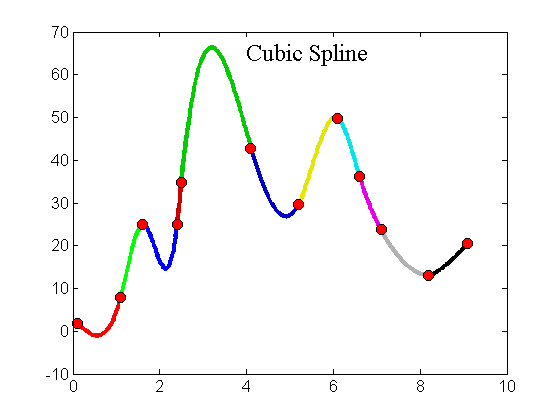
\includegraphics{./images/cubic_spline.png}
\caption{\label{fig:cubic-spline}Cada segmento de uma spline cúbica é um
polinômio de grau 3 diferente.}
\end{figure}

\section{Suavização}\label{suavizacao}

A técnica de suavização é muito semelhante a interpolação, inclusive o
método spline também é aplicado, com algumas modificações de forma que
nem todos os pontos fornecidos serão nós.

Na spline de suavização (ou aproximação), os pontos fornecidos são
separados entre os nós, onde a função deve passar e pontos de controle,
que são utilizados para controlar a curvatura da função nestes pontos.

Estas suavizações são principalmente utilizadas quando se possui muitas
observações sujeitas a ruídos, de forma que uma interpolação entre todos
os pontos seria tanto impraticável quanto sem sentido. O que se deseja,
portanto, é uma função \textbf{aproximada} que melhor descreva o
processo sob análise.

Um ponto em comum entre estas técnicas é o parâmetro de suavização,
ausente, na interpolação, que controla a ``suavidade'' da função
estimada.

\begin{figure}
\centering
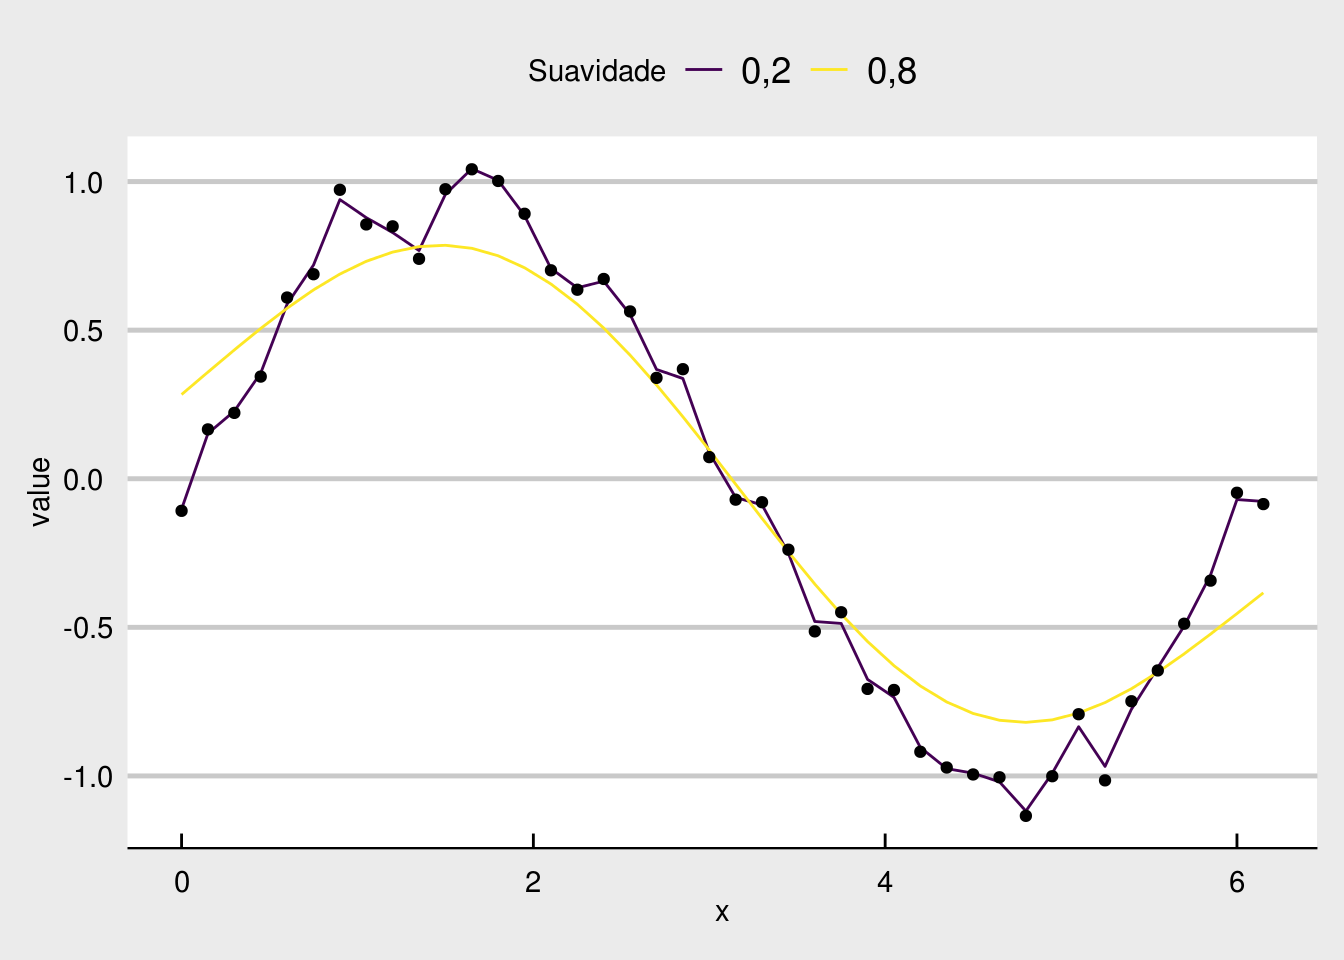
\includegraphics{06-metodos-calibracao_files/figure-latex/suavizacao-1.pdf}
\caption{\label{fig:suavizacao}Menor parâmetro de suavização gera
granularidade na curva.}
\end{figure}

\section{Parametrização}\label{parametrizacao}

E por fim as técnicas de parametrização. Nesta categoria estão diversos
conhecidos modelos de superfícies de volatilidade implícita, dentre eles
os modelos de \citet{Heston1993}, Volatilidade Local de
\citet{Dupire1994} e SVI de \citet{Gatheral2004}.

Em comum, estes modelos tentam parametrizar a superfície, e por
conseguinte o smile de volatilidade, de acordo com alguma função, em
geral não-linear, que possui características condizentes com a teoria de
precificão de derivativos e também a observação empírica das
superfícies.

Por exemplo, a parametrização \emph{raw} da SVI possui a seguinte forma
para a \textbf{variância total}\footnote{A variância total é definida
  pelo produto entre a variância implícita e o tempo para expiração,
  \(w=\sigma^2_{imp}\cdot\tau\).} :

\[ w(k) = a + b\left(\rho(k-m)+\sqrt{(k-m)^2 + \sigma^2}\right)\]

que fornece um espaço de cinco parâmetros
\(\chi_B=\{a, b, \rho, m, \sigma\}\) que definem o smile e devem,
portanto, serem calibrados a partir de dados observados no mercado.

O procedimento de calibração consiste em encontrar o conjunto de
parâmetros que minimizam uma função perda entre a volatilidade prevista
pelo modelo e os dados de mercado, enquanto satisfazem algumas
restrições adicionais, como ``ausência de arbitragem'', suavidade, etc.
Trata-se, via de regra, de problemas de otimização não-linear com
restrições de inequalidade também não-lineares.

\subsection{Função perda}\label{funcao-perda}

A função perda, ou função de calibração pode ser definida de diversas
maneiras, de forma geral, para uma determinada maturidade, ela toma a
forma:

\[L=\sum\limits_{i=1}^n\lambda_i||\hat w(k_i)-w_{imp}(k_i)||\] onde
\(||\cdot||\) é alguma medida de norma, sendo a mais conhecida o
quadrado das diferenças, dando origem a minimização do erro quadrático
médio (RMSE). Para este smile sendo calibrado existem \(n\) strikes
(\(k_i\)) e suas volatilidades implícitas observadas são
\(w_{imp}(k_i)\). A resposta do modelo para um determinado strike é
\(\hat w(k_i)\) e \(\lambda_i\) são os pesos dados na função perda para
cada um destes strikes.

Os pesos \(\lambda_i\) são utilizados para ponderar as observações das
volatilidades mais importantes para o cálculo, onde se deseja que a
curva ajustada possua um menor erro. Em geral, estes pesos são calculado
como inversamente proporcionais:

\begin{itemize}
\tightlist
\item
  ao quadrado dos \emph{spreads bid-ask}, para dar mais importância às
  opções mais líquidas
\item
  ao quadrado da grega vega calculada a partir do modelo BSM
\end{itemize}

\subsection{Otimizadores}\label{otimizadores}

Os otimizadores são os algoritmos pelos quais o problema de minimização
posto é resolvido. Se a função perda é convexa, e ela deve ser
construída de forma a ser, mesmo que não estritamente, então ela possui
um ou mais pontos de mínimo onde o gradiente desta função é igual a
zero. O que os otimizadores fazem é buscar o conjunto de parâmetros que
minimizam a função perda e atendem as restrições impostas
simultaneamente. Os otimizadores podem ser classificados em dois grandes
grupos, globais e locais.

Algoritmos locais dependem de uma estimativa inicial dos parâmetros para
começarem a busca pelo mínimo. Seguindo uma regra utilizando-se o
gradiente da função ou alguma heurística, estes otimizadores caminham em
direção ao ponto de mínimo mais próximo da estimativa inicial, daí o
nome ``local''. Como desvantagem destes otimizadores é a mais evidente é
que se a função perda for altamente não-linear, com diversos pontos de
mínimo local, este otimizador pode ficar preso em um destes pontos sem
nunca, no entanto, encontrar o mínimo global. Eles são, portanto muito
sensíveis à estimativa inicial dos parâmetros.

Por sua vez, otimizadores globais buscam mapear todo o espaço factível
para os parâmetros e encontrar o ponto mínimo da função perda dentro
deste espaço. Estes algoritmos não dependem de estimativas iniciais, uma
vez que tentarão avaliar o espaço completo. São utilizados quando o
problema de minimização é não-linear e possui múltiplos pontos de mínimo
local. Estes algoritmos usam alguma forma de heurística para encontrar a
região onde o mínimo global está localizado, mas são, em geral,
ineficientes em apontar rapidamente onde este ponto de mínimo se
encontra com precisão. Por esta razão, é frequente a utilização de
otimizadores globais com um posterior refinamento de sua solução por
algum algoritmo local.

Abaixo apresentamos alguns exemplos mais comuns de otimizadores, tanto
locais quanto globais:

\begin{itemize}
\item
  \textbf{Gauss-Newton}: Este método é utilizado para encontrar as
  raízes de alguma função. Para encontrar o ponto de mínimo da função
  perda, precisa-se encontrar as raízes do gradiente desta função,
  portanto o método de Newton em otimização faz uso da função gradiente.
  Este é um método de otimização local.
\item
  \textbf{Levenberg-Marquardt}: Método muito utilizado para problemas
  não-lineares, ele parte de uma modificação ao método de Gauss-Newton
  ao introduzir um fator de amortecimento calculado iterativamente.
\item
  \textbf{L-BFGS-B}: BFGS é um método conhecido como quasi-Newton, onde
  não é necessário calcular a Hessiana do problema, ela é aproximada a
  partir do próprio gradiente. É bastante utilizado para resolver
  problemas não-lineares e em sua versão L-BFGS-B pode lidar com
  restrições do tipo \emph{box}, intervalo dos parâmetros é fixo.
\item
  \textbf{Nelder-Mead}: Este é um método livre do uso de gradiente, já
  que usa uma heurística para construir um simplex e a partir deste
  ``procurar'' por um mínimo. Bastante utilizado quando a função
  objetivo pode não ser diferenciável. Faz uso de um simplex inicial,
  que pode ser grande o suficiente para encampar o mínimo global,
  entretanto, não se classifica como um otimizador global.
\item
  \textbf{Algoritmo Genético}: Este método utiliza conceitos da seleção
  natural para gerar os resultados da otimização. É um otimizador
  global, no sentido que independe de uma estimativa inicial de
  parâmetros e faz uma busca por todo o espaço factível. Em um algoritmo
  genético, uma população aleatória inicial de parâmetros é criada e a
  partir desta, as gerações evoluem conforme mutações e
  \emph{cross-over} de características e é avaliado o \emph{fitness} de
  cada conjunto de parâmetros até um deles ser considerado adequado.
\item
  \textbf{Evolução Diferencial}: É um método de otimização global, assim
  como o Algoritmo Genético e o Enxame de Partículas. Sua diferença
  reside no fato de que sua população inicial é constantemente avaliada
  e deslocada de posição. Se o agente obtiver uma situação melhor (menor
  valor para a função perda) na nova posição, esta agora faz parte da
  população. Desta forma os agentes, antes espalhados pelo espaço
  factível dos parâmetros, tendem a convergir para um ponto com o menor
  valor da função perda.
\item
  \textbf{Enxame de Partículas}: Do inglês, \emph{Particle Swarm
  Optimization - PSO} este método é semelhante ao DE \emph{(Differential
  Evolution)} porém as partículas (o equivalente dos agentes no DE)
  matém informações sobre a posição da melhor partícula até então, de
  forma a fazer com que as partículas tendam para a melhor solução.
\end{itemize}

\section{Conclusão}\label{conclusao-2}

Dependendo do objetivo da aplicação, superfícies de volatilidade podem
ser interpoladas, suavizadas ou parametrizadas. A parametrização tem
recebido especial interesse pois pode, ao mesmo tempo que garante uma
superfície livre de arbitragem estática se devidamente construída,
ajustar-se muito bem aos dados observados e gerar distribuições neutras
ao risco implícitas factíveis.

Para gerar uma superfície parametrizada, primeiramente é necessário um
modelo teórico com propriedades desejáveis e que se ajuste aos dados de
mercado quando calibrado. Escolhido este modelo paramétrico, passa-se a
calibração do mesmo onde exsitem diversas opções de escolha entre
otimizadores. Ao final do processo teremos um modelo de superfície
devidamente parametrizado com valores que melhor se ajustam segundo
alguma função perda escolhida.

Com a superfície de volatilidade calibrada, as aplicações possíveis
incluem a precificação de derivativos, gerenciamento de risco,
simulações de Monte Carlo, análises de stress, entre outras.

\hypertarget{svi}{\chapter{Calibrando uma SVI}\label{svi}}

Neste capítulo iremos mostrar como fazer uma calibração de um smile SVI
baseado nos trabalhos de \citep{Gatheral2004} e \citep{DeMarco2009}.
Escolheremos apenas uma fatia da superfície de volatilidade, fixando o
tempo para expiração (maturidade) e coletando as volatilidades
implícitas para diversos strikes.

Como já apresentado em posts anteriores, existem diversas formas de
interpolar, extrapolar, parametrizar e calibrar smiles de volatilidade.
Exsitem vantagens e desvantagens para cada método. Neste post iremos
fixar nossa atenção no modelo paramétrico de smile chamado SVI -
Stochastic Volatility Inspired - uma forma que une a ``simplicidade'' de
um modelo paramétrico com o poder de adesão aos dados de mercado dos
modelos de volatilidade estocástica (i.e.~Heston, SABR e afins).

Chamar o modelo SVI de simples é puro eufemismo, ele é um modelo
poderoso, com fundamento teórico avançado e diversos detalhes para sua
calibração.

\section{Modelo SVI}\label{modelo-svi}

Este modelo foi apresentado por
\href{https://mfe.baruch.cuny.edu/jgatheral/}{Jim Gatheral} na
conferência \emph{Global Derivatives \& Risk Management 2004} e foi bem
recebido pelos profissionais de mercado interessados em superfícies de
volatilidade para \emph{equities}, principalmente.

O modelo possui duas propriedades que são as razões para sua
popularidade. Ele satisfaz a fórmula do momento de \citet{Lee2004}, que
é um resultado independente de modelo que especifica os limites
assintóticos para um \emph{smile} de volatilidade implícita. Portanto, o
modelo SVI é válido para extrapolação além da região central dos dados
disponíveis. Além disso, afirma-se que o modelo SVI é relativamente
fácil de calibrar para dados de mercado, de modo que a superfície de
volatilidade implícita correspondente é livre de arbitragem de
calendário. As condições que garantem a ausência de arbitragem de
borboleta forma resolvidas em um segundo artigo por
\citet{Gatheral2014}.

No SVI é possível se estabelecer condições explícitas em seus
parâmetros, de modo que o modelo não gere preços onde oportunidades de
\protect\hyperlink{arbestatica}{arbitragem estáticas} possam ocorrer. A
calibração para dados reais de mercado requer algoritmos de otimização
não-linear e pode ser bastante demorada. Mais recentemente, um método
para calibração que usa a estrutura inerente do modelo para reduzir as
dimensões do problema de otimização foi desenvolvido em
\citet{DeMarco2009}.

A parametrização conhecida como \emph{RAW} do SVI é apresentada na
equação \eqref{eq:rawsvi}, seguindo a notação já introduzida
\protect\hyperlink{smile}{anteriormente}, portanto, estamos modelando a
\textbf{variância total} implícita para um determinado prazo. Para
diferentes maturidades, teremos diferentes conjuntos de parâmetros.

\begin{equation}
w(k) = a + b\left(\rho(k-m)+\sqrt{(k-m)^2 + \sigma^2}\right)
\label{eq:rawsvi}
\end{equation}

onde: \(a \in \mathbb R\), \(b \geq 0\), \(|\rho| < 1\),
\(m \in \mathbb R\), \(\sigma > 0\), e
\(a+b \sigma\sqrt{1 − \rho^2} \geq 0\) para garantir que
\(\min w(k)>0, \, \forall k \in \mathbb R\).

\section{Restrições de
não-arbitragem}\label{restricoes-de-nao-arbitragem}

Antes de demonstrar a restrição imposta aos parâmetros \(b\) e \(\rho\)
em função dos limites de inclinação das asas do \emph{smile}, vamos
derivar as expressões para \(w\prime(k)\) e \(w\prime\prime(k)\) que nos
serão úteis na demonstração.

A expressão para \(w\prime(k)\) é bastante simples:

\begin{equation}
w\prime(k) = b \left[\rho + \frac{(k-m)}{\sqrt{(k-m)^2+\sigma^2}}\right]
\label{eq:wk}
\end{equation}

Derivando novamente a equação \eqref{eq:wk} em relação a \(k\) teremos uma
expressão ainda mais simples, mesmo que após alguma manipulação
algébrica um tanto tediosa\footnote{A resolução desta derivada é uma
  simples regra da divisão, entretanto a simplificação do resultado pede
  alguma manipulação algébrica. É possível utilizar sistemas de
  computação simbólica, o qual recomendamos o
  \href{https://live.sympy.org/}{SymPy}}, e resulta em:

\begin{equation}
w\prime\prime(k)=\frac{b\sigma^2}{[(k-m)^2+\sigma^2]^{3/2}}
\label{eq:wkk}
\end{equation}

onde, se considerarmos \(b>0\) temos que
\(w\prime\prime(k)>0, \,\forall k\in \mathbb R\), ou seja, o
\emph{smile} de volatilidade definido pela equação \eqref{eq:rawsvi} é
\textbf{estritamente} convexo.

\citet{Rogers2010} definiram os limites possíveis para a inclinação das
asas em função do tempo para expiração, provando que o \emph{smile}
tende a ficar mais horizontal a medida que o prazo aumenta. Este limite
pode ser escrito da seguinte forma e é uma \textbf{condição necessária}
para a ausência de arbitragem:

\begin{equation}
|w\prime(k)|\leq \frac{4}{\tau} \qquad \forall k \in \mathbb R, \quad \forall \tau \in (0, \infty)
\label{eq:rogers}
\end{equation}

Sendo o \emph{smile} convexo, suas máximas inclinações ocorrem quando
\(k\rightarrow \pm \infty\). Portanto, deve-se avaliar a restrição dada
pela equação \eqref{eq:rogers} nestes limites da seguinte maneira:

\begin{align}
\lim\limits_{k\rightarrow\infty}w\prime(k)&=b(1+\rho)\geq 0\\
\lim\limits_{k\rightarrow-\infty}w\prime(k)&=-b(1-\rho)\leq 0
\end{align}

que satisfazendo estas duas relações ao mesmo tempo em que se restringe
os parâmetros \(b\) e \(\rho\) através da inequalidade de Rogers e
Tehranchi nos garante o seguinte resultado para um SVI \textbf{livre de
arbitragem de travas}.

\begin{equation}
b(1+|\rho|)\leq\frac{4}{\tau}
\label{eq:trava}
\end{equation}

Para garantir que a superfície gerada está livre de arbitragem do tipo
borboleta deve-se primeiramente definir uma função\footnote{Condições
  para ausência de arbitragem do tipo borboleta em um SVI estão
  detalhadas na seção 2.2 do artigo de \citet{Gatheral2014}.}
\(g: \mathbb R\rightarrow \mathbb R\), tal que:

\begin{equation}
g(k)=\left(1-\frac{kw\prime(k)}{2w(k)}\right)^2-\frac{w\prime(k)^2}{4}\left(\frac{1}{w(k)}+\frac{1}{4}\right)+\frac{w\prime\prime(k)}{2}
\label{eq:g}
\end{equation}

e seguir o lema :

\textbf{Lema 1} Uma fatia da superfície de volatilidade está livre de
arbitragem do tipo borboleta se, e somente se, \(g(k) \geq 0\) para todo
\(k \in \mathbb R\) e
\(\lim\limits_{k\rightarrow+\infty}d_1(k)=-\infty\).

Infelizmente, a natureza altamente não-linear da função \(g(k)\)
impossibilita a derivação de restrições gerais aos parâmetros do SVI. A
forma mais simples de eliminar arbitragem do tipo borbobleta é incluir a
restrição \(g(k) \geq 0\) na função perda e proceder com a calibração
dos parâmetros.

\section{Reparametrização
Quasi-explicit}\label{reparametrizacao-quasi-explicit}

Um dos problemas mais marcantes com a calibração do SVI dado pela
equação \eqref{eq:rawsvi} é sua natureza altamente não-linear que gera
inúmeros pontos de mínimo locais. Mesmo em um ambiente simulado, um
típico otimizador de \protect\hyperlink{calibracao}{mínimos quadrados}
como Levenberg-Marquardt não consegue chegar ao mínimo global, onde a
função perda é igual a zero. A solução encontrada é dependente dos
valores iniciais inputados ao otimizador e a robustez do conjunto de
parâmetros encontrados não é garantida.

Uma forma de contornar este problema pode ser a utilização de
otimizadores globais, como algortimos genéticos, em um primeiro estágio
e então o refinamento desta solução através de um otimizador local (LM,
por exemplo).

Outra forma, adotada em \citet{DeMarco2009} é a reparametrização da
equação \eqref{eq:rawsvi} de forma que esta possa ser tratada como um
prolema linear. Para tanto, considere a seguinte troca de variáveis:

\begin{equation}
y = \frac{k-m}{\sigma}
\end{equation}

então a parametrização \emph{RAW} do SVI se torna.

\begin{equation}
w(y) = a + b\sigma\left(\rho y + \sqrt{y^2 + 1}\right)
\end{equation}

Definindo agora as seguintes variáveis reparametrizadas é possível
reduzir a dimensão de parâmetros de um SVI de 5 para apenas 3:

\begin{align}
c = &b\sigma\\
d = &\rho b \sigma
\end{align}

\begin{equation}
w(y)=a+dy+c\sqrt{y^2+1}
\label{eq:quasiexplicit}
\end{equation}

Portanto, para um par fixo de \((m, \sigma)\) nosso problema reduzido é:

\begin{equation}
P_{m, \sigma}:=\min\limits_{a, c, d \in D}f_y(a, c, d)
\label{eq:reduzido}
\end{equation}

onde \(f_y(\cdot)\) é a função objetivo da reparametrização, e é dada
pela seguinte equação:

\begin{equation}
f_y(a, c, d)=\sum_{i=1}^{n}\left[w(y_i)-\tilde w_i\right]^2
\label{eq:fy}
\end{equation}

onde \(\tilde w_i\) é a variância total observada correspondente ao
\emph{moneyness} \(k_i\).

O domínio \(D\) dos parâmetros \(\{a, c, d\}\) é encontrado a partir do
limite imposto por \eqref{eq:trava}.

\begin{equation}
    D =  
    \begin{cases}
    0 \leq c \leq 4\sigma\\
    |d| \leq c \quad \text{e}\quad |d| \leq 4\sigma - c\\
    0 \leq a \leq \max\{\tilde w_i\}\\
    \end{cases}
    \label{eq:D}
\end{equation}

O problema reduzido dado pela equação \eqref{eq:reduzido}, é um típico
problema de \textbf{mínimos quadrados} com restrições lineares. Este
problema, por ser convexo, admite uma única solução interior (se
existente) que será o mínimo global para este problema e é encontrada
através do gradiente da função objetivo igualando-o a zero,
\(\nabla f_y = 0\). Esta equação gera um sistema linear nos parâmetros
\(a, c, d\) que pode ser explicitamente resolvido. Caso a solução
encontrada para este problema esteja contida no domínio \(D\), esta
solução é interior e é o mínimo desejado, caso contrário, deve-se
percorrer o perímetro do domínio e encontrar o menor valor da função
objetivo que será uma solução de canto.

Seja \((a^*, c^*, d^*)\) a solução de \eqref{eq:reduzido} e
\((a^*, b^*, \rho^*)\) os correspondentes parâmetros originais
recuperados, então o problema completo de calibração é:

\begin{equation}
P:=\min\limits_{m, \sigma}\sum_{i=1}^n (w_*(k_i)-\tilde w_i)^2
\label{eq:completo}
\end{equation}

onde
\(w_*(k)=a^*+b^*\left(\rho^*(k-m)+\sqrt{(k-m)^2 + \sigma^2}\right)\).

O problema completo, \eqref{eq:completo} é um problema em apenas duas
dimensões, \((m, \sigma)\) e não-linear, que deve ser abordado através
de algum tipo de otimizador global.

\subsection{Solução explícita do problema reduzido}\label{pq}

Nesta seção apresentaremos a solução, sem considerar as restrições
impostas em \eqref{eq:D} para o problema reduzido em \eqref{eq:reduzido},
algo omitido em \citet{DeMarco2009}. Esta seção é opcional para o leitor
atento que já percebeu a semelhança entre o problema reduzido e um
típico problema de regressão linear múltipla.

Para encontrar o conjunto de parâmetros \((a^*, c^*, d^*)\) que
representam os valores ótimos na equação \eqref{eq:reduzido}, devemos
resolver o seguinte sistema de equações:

\begin{equation}
\nabla f_y = \left[
    \begin{array}{c}
        \partial f_y / \partial a\\ 
        \partial f_y / \partial d\\
        \partial f_y / \partial c
    \end{array} 
\right] = \boldsymbol{0}
\label{eq:gradiente}
\end{equation}

Cada uma das derivadas parciais da equação acima quando igualadas a zero
dão origem ao sistema linear apresentado abaixo:

\begin{equation}
\scriptsize
\begin{bmatrix}
&n &\sum y_i &\sum\sqrt{y_i^2+1}\\
&\sum y_i &\sum y_i^2 &\sum(y_i\sqrt{y_i^2+1})\\
&\sum\sqrt{y_i^2+1} &\sum(y_i\sqrt{y_i^2+1}) &\sum(y_i^2+1)\\
\end{bmatrix}
\cdot
\begin{bmatrix}
a \\
d \\
c
\end{bmatrix}
=
\begin{bmatrix}
\sum\tilde w_i \\
\sum \tilde w_i y_i \\
\sum(\tilde w_i\sqrt{y_i^2+1})
\end{bmatrix}
\label{eq:linear}
\end{equation}

Portanto, o problema reduzido pode ser resolvido através de um sistema
linear de ordem 3 sob restrições também lineares.

\section{Algoritmo}\label{algoritmo}

A otimização para encontrar os parâmetros ótimos de um SVI dadas
observações de mercado e a técnica de calibração \textbf{Quasi-explicit}
de \citet{DeMarco2009} pode ser resumida nos seguintes passos:

\begin{enumerate}
\def\labelenumi{\arabic{enumi}.}
\item
  Definir valores iniciais para os parâmetros \((m, \sigma)\),
\item
  Iniciar algum otimizador global com estes parâmetros e resolver o
  problema completo \eqref{eq:completo}

  2.1 Dentro da otimização global, resolver o problema reduzido
  \eqref{eq:reduzido} para os parâmetros \((m, \sigma)\) dados,
\item
  Na convergência do problema completo do passo 2, otimizar uma última
  vez o problema reduzido,
\item
  Recuperar os parâmetros \((a, b, \rho, m, \sigma)\)
\end{enumerate}

A escolha dos otimizadores fica a cargo pessoal, sendo sugerido testar
vários para o mesmo problema. Eventualmente, para um determinado
\emph{smile} um otimizador pode se mostrar melhor que outro que vinha
sendo utilizado em outras ocasiões.

Nos testes realizados pelo \href{http://clubedefinancas.com.br}{Clube de
Finanças}, entre os otimizadores globais para o problema completo
utilizamos
\href{https://cran.r-project.org/package=GA}{\textbf{Algoritmos
Genéticos}},
\href{https://www.rdocumentation.org/packages/stats/versions/3.5.2/topics/constrOptim}{\textbf{Nelder-Mead
restrito}} e um
\href{https://cran.r-project.org/package=Rsolnp}{\textbf{Método
não-linear generalizado}}. Para o problema reduzido, apesar de ser
linear, o método de Nelder-Mead restrito se mostrou tão eficiente quanto
e de mais fácil implementação. Se o objetivo for fazer uma calibração
direta, dos cinco parâmetros ao mesmo tempo, uma combinação de
otimizador global em primeiro estágio e o método de Levenberg-Marquardt
restrito para refinamento da solução é o ideal.

\section{Resultados}\label{resultados}

A seguir apresentamos um \emph{smile} de referência para a calibração,
obtido de
\href{http://www.ivolatility.com/doc/usa/IV_Raw_Delta_surface.csv}{ivolatility.com}
e então partimos para diferentes técnicas de calibração de um SVI. Os
códigos em \href{https://cran.r-project.org/}{R} também estão
apresentados ao longo do texto para melhor compreensão e estudo do
leitor.

Os dados utilizados neste exemplo estão apresentados na tabela
\ref{tab:dados} abaixo. Esta é uma típica apresentação de um
\emph{slice} de superfície, ou seja, dados para um \emph{smile} apenas.
As principais variáveis são: a data em que os dados foram coletados
(date), o preço de fechamento do ativo (stock\_price), o prazo para
expiração em dias (period), e medidas de moneyness como delta,
\emph{strike} e o próprio \emph{moneyness}, além é claro da volatilidade
implícita (iv) retirada do mercado.

\begin{table}[t]

\caption{\label{tab:dados}Dados reais para exemplo de calibração de uma SVI.}
\centering
\fontsize{14}{16}\selectfont
\begin{tabular}{lllrrrrrr}
\toprule
date & symbol & exchange & stock\_price\_for\_iv & period & delta & moneyness & strike & iv\\
\midrule
2017-09-21 & IWM & NYSEArca & 143.73 & 30 & 10 & 0.03 & 148.41 & 0.09\\
2017-09-21 & IWM & NYSEArca & 143.73 & 30 & 15 & 0.03 & 147.49 & 0.09\\
2017-09-21 & IWM & NYSEArca & 143.73 & 30 & 20 & 0.02 & 146.80 & 0.09\\
2017-09-21 & IWM & NYSEArca & 143.73 & 30 & 25 & 0.02 & 146.21 & 0.09\\
2017-09-21 & IWM & NYSEArca & 143.73 & 30 & 30 & 0.01 & 145.69 & 0.09\\
\addlinespace
2017-09-21 & IWM & NYSEArca & 143.73 & 30 & 35 & 0.01 & 145.19 & 0.10\\
2017-09-21 & IWM & NYSEArca & 143.73 & 30 & 40 & 0.01 & 144.69 & 0.10\\
2017-09-21 & IWM & NYSEArca & 143.73 & 30 & 45 & 0.00 & 144.18 & 0.10\\
2017-09-21 & IWM & NYSEArca & 143.73 & 30 & 50 & 0.00 & 143.66 & 0.10\\
2017-09-21 & IWM & NYSEArca & 143.73 & 30 & 55 & 0.00 & 143.12 & 0.11\\
\addlinespace
2017-09-21 & IWM & NYSEArca & 143.73 & 30 & 60 & -0.01 & 142.53 & 0.11\\
2017-09-21 & IWM & NYSEArca & 143.73 & 30 & 65 & -0.01 & 141.88 & 0.11\\
2017-09-21 & IWM & NYSEArca & 143.73 & 30 & 70 & -0.02 & 141.13 & 0.12\\
2017-09-21 & IWM & NYSEArca & 143.73 & 30 & 75 & -0.02 & 140.26 & 0.13\\
2017-09-21 & IWM & NYSEArca & 143.73 & 30 & 80 & -0.03 & 139.16 & 0.13\\
\addlinespace
2017-09-21 & IWM & NYSEArca & 143.73 & 30 & 85 & -0.04 & 137.66 & 0.14\\
2017-09-21 & IWM & NYSEArca & 143.73 & 30 & 90 & -0.06 & 135.32 & 0.16\\
\bottomrule
\end{tabular}
\end{table}

Esta tabela poderia conter (de fato contém no arquivo original) outros
períodos de expiração, e neste caso uma das colunas de \emph{moneyness}
começa a se repetir, no caso seria o delta pois baixamos uma tabela de
volatilidades implícitas por delta. Assim, em uma tabela simples em
formato
\href{http://vita.had.co.nz/papers/tidy-data.html}{\texttt{tidy}} é
possível armazenar informações de uma superfície inteira, a qual de
outra forma necessitaria de um arranjo em 3 dimensões.

Ressaltamos aqui que a unidade de volatilidade implícita está em
percentuais \textbf{ao ano}, equanto que nosso período é de dias
corridos. É necessário harmonizar estas medidas de forma que, para
volatiliades dadas em percentual ao ano, o período também seja dado em
\textbf{anos}. Logo nosso \(\tau = 30/365\), ou seja, 0.08219.

Demonstraremos aqui os resultados para a calibração de uma \emph{RAW
SVI} pelos métodos ``Direto'', ``GA'', ``Quasi-NM'' e ``Quasi-PQ'',
abaixo explicados.

O método ``Direto'' é uma calibração direta através de um algoritmo de
\textbf{Levenberg-Marquardt} da equação \eqref{eq:rawsvi}, ou seja, não
existe reparametrização \emph{Quasi-explicit} e o problema resolvido é
não-linear em 5 dimensões. São realizadas 10 calibrações com estimativas
iniciais dos parâmetros aleatórias, mas dentro de seus respectivos
domínios. A melhor solução, aquela com o menor valor para a função
objetivo, é selecionada. Todos os outros métodos utilizam a
reparametrização, ocorrendo variações apenas nos algoritmos de
otimização utilizados nos problemas reduzido e completo.

A calibração ``GA'' faz uso do otimizador global de \textbf{algoritmos
genéticos} para o problema completo, ou seja, para estimar o par
\((m, \sigma)\) que corresponde ao mínimo global. Após, o problema
reduzido é resolvido através do algoritmo de \textbf{Nelder-Mead}. Este
método é robusto, pois o algoritmo genético tem grande probabilidade de
encontrar a região onde se encontra o mínimo global e não ficar preso
localmente. Entretanto a robustez ocorre as expensas do tempo de
computação.

Os métodos ditos ``Quasi'' diferem entre si na resolução do problema
reduzido. Enquanto ``PQ'' remete a \textbf{programação quadrática} e faz
uso da resolução do sistema linear apresentado na equação
\eqref{eq:linear} com as restrições impostas por \eqref{eq:D}, o método
``Quasi-NM'' utiliza o método de \textbf{Nelder-Mead} com restrições
para a resolução deste mesmo problema reduzido. Em ambos os métodos, o
problema completo é resolvido com um algoritmo de Nelder-Mead com 50
reinicializações das estimativas iniciais dos parâmetros
\((m, \sigma)\), o que causa algum impacto no tempo de computação destes
métodos.

\begin{Shaded}
\begin{Highlighting}[]
\NormalTok{smile <-}\StringTok{ }\NormalTok{dados }\OperatorTok\StringTok{ }
\StringTok{  }\KeywordTok{mutate}\NormalTok{(}\DataTypeTok{tau =}\NormalTok{ period }\OperatorTok{/}\StringTok{ }\DecValTok{365}\NormalTok{) }\OperatorTok\StringTok{ }
\StringTok{  }\KeywordTok{select}\NormalTok{(moneyness, iv, tau)}

\NormalTok{par_names <-}\StringTok{ }\KeywordTok{factor}\NormalTok{(}\KeywordTok{c}\NormalTok{(}\StringTok{"a"}\NormalTok{, }\StringTok{"b"}\NormalTok{, }\StringTok{"$}\CharTok{\textbackslash{}\textbackslash{}}\StringTok{rho$"}\NormalTok{, }\StringTok{"m"}\NormalTok{, }\StringTok{"$}\CharTok{\textbackslash{}\textbackslash{}}\StringTok{sigma$"}\NormalTok{),}
                    \DataTypeTok{levels =} \KeywordTok{c}\NormalTok{(}\StringTok{"a"}\NormalTok{, }\StringTok{"b"}\NormalTok{, }\StringTok{"$}\CharTok{\textbackslash{}\textbackslash{}}\StringTok{rho$"}\NormalTok{, }\StringTok{"m"}\NormalTok{, }\StringTok{"$}\CharTok{\textbackslash{}\textbackslash{}}\StringTok{sigma$"}\NormalTok{))}
\NormalTok{k <-}\StringTok{ }\NormalTok{smile}\OperatorTok{$}\NormalTok{moneyness}
\NormalTok{w <-}\StringTok{ }\NormalTok{smile}\OperatorTok{$}\NormalTok{iv}\OperatorTok{^}\DecValTok{2} \OperatorTok{*}\StringTok{ }\NormalTok{smile}\OperatorTok{$}\NormalTok{tau}

\NormalTok{init_direct <-}\StringTok{ }\KeywordTok{proc.time}\NormalTok{()}
\NormalTok{par_direct <-}\StringTok{ }\KeywordTok{svi_fit_direct}\NormalTok{(k, w)}
\NormalTok{end_direct <-}\StringTok{ }\KeywordTok{proc.time}\NormalTok{()}
\NormalTok{time_direct <-}\StringTok{ }\NormalTok{end_direct }\OperatorTok{-}\StringTok{ }\NormalTok{init_direct }

\NormalTok{init_ga <-}\StringTok{ }\KeywordTok{proc.time}\NormalTok{()}
\NormalTok{par_ga <-}\StringTok{ }\KeywordTok{svi_fit_ga}\NormalTok{(k, w)}
\NormalTok{end_ga <-}\StringTok{ }\KeywordTok{proc.time}\NormalTok{()}
\NormalTok{time_ga <-}\StringTok{ }\NormalTok{end_ga }\OperatorTok{-}\StringTok{ }\NormalTok{init_ga }

\NormalTok{init_quasipq <-}\StringTok{ }\KeywordTok{proc.time}\NormalTok{()}
\NormalTok{par_quasipq <-}\StringTok{ }\KeywordTok{svi_fit_quasi}\NormalTok{(k, w, }\DataTypeTok{inner =} \StringTok{"quadprog"}\NormalTok{)}
\NormalTok{end_quasipq <-}\StringTok{ }\KeywordTok{proc.time}\NormalTok{()}
\NormalTok{time_quasipq <-}\StringTok{ }\NormalTok{end_quasipq }\OperatorTok{-}\StringTok{ }\NormalTok{init_quasipq }

\NormalTok{init_quasinm <-}\StringTok{ }\KeywordTok{proc.time}\NormalTok{()}
\NormalTok{par_quasinm <-}\StringTok{ }\KeywordTok{svi_fit_quasi}\NormalTok{(k, w)}
\NormalTok{end_quasinm <-}\StringTok{ }\KeywordTok{proc.time}\NormalTok{()}
\NormalTok{time_quasinm <-}\StringTok{ }\NormalTok{end_quasinm }\OperatorTok{-}\StringTok{ }\NormalTok{init_quasinm }

\NormalTok{iv_direct <-}\StringTok{ }\KeywordTok{sqrt}\NormalTok{(}\KeywordTok{svi_fun}\NormalTok{(par_direct}\OperatorTok{$}\NormalTok{par[[}\DecValTok{1}\NormalTok{]], k) }\OperatorTok{/}\StringTok{ }\NormalTok{smile}\OperatorTok{$}\NormalTok{tau)}
\NormalTok{iv_ga <-}\StringTok{ }\KeywordTok{sqrt}\NormalTok{(}\KeywordTok{svi_fun}\NormalTok{(par_ga}\OperatorTok{$}\NormalTok{par[[}\DecValTok{1}\NormalTok{]], k) }\OperatorTok{/}\StringTok{ }\NormalTok{smile}\OperatorTok{$}\NormalTok{tau)}
\NormalTok{iv_quasipq <-}\StringTok{ }\KeywordTok{sqrt}\NormalTok{(}\KeywordTok{svi_fun}\NormalTok{(par_quasipq}\OperatorTok{$}\NormalTok{par[[}\DecValTok{1}\NormalTok{]], k) }\OperatorTok{/}\StringTok{ }\NormalTok{smile}\OperatorTok{$}\NormalTok{tau)}
\NormalTok{iv_quasinm <-}\StringTok{ }\KeywordTok{sqrt}\NormalTok{(}\KeywordTok{svi_fun}\NormalTok{(par_quasinm}\OperatorTok{$}\NormalTok{par[[}\DecValTok{1}\NormalTok{]], k) }\OperatorTok{/}\StringTok{ }\NormalTok{smile}\OperatorTok{$}\NormalTok{tau)}

\NormalTok{plot_tbl <-}\StringTok{ }\KeywordTok{tibble}\NormalTok{(}\DataTypeTok{k =}\NormalTok{ k,}
              \DataTypeTok{Direct =}\NormalTok{ iv_direct,}
              \DataTypeTok{GA =}\NormalTok{ iv_ga,}
              \DataTypeTok{QuasiPQ =}\NormalTok{ iv_quasipq,}
              \DataTypeTok{QuasiNM =}\NormalTok{ iv_quasinm,}
              \DataTypeTok{observed =}\NormalTok{ smile}\OperatorTok{$}\NormalTok{iv) }\OperatorTok\StringTok{ }
\StringTok{  }\KeywordTok{gather}\NormalTok{(}\DataTypeTok{key =}\NormalTok{ method, }\DataTypeTok{value =}\NormalTok{ iv, }\OperatorTok{-}\KeywordTok{c}\NormalTok{(k, observed))}

\NormalTok{par_tbl <-}\StringTok{ }\KeywordTok{bind_rows}\NormalTok{(par_direct, par_ga, par_quasipq, par_quasinm) }\OperatorTok\StringTok{ }
\StringTok{  }\KeywordTok{select}\NormalTok{(method, par) }\OperatorTok\StringTok{ }
\StringTok{  }\KeywordTok{mutate}\NormalTok{(}\DataTypeTok{method =} \KeywordTok{c}\NormalTok{(}\StringTok{"Direct"}\NormalTok{, }\StringTok{"GA"}\NormalTok{, }\StringTok{"QuasiPQ"}\NormalTok{, }\StringTok{"QuasiNM"}\NormalTok{)) }\OperatorTok\StringTok{ }
\StringTok{  }\KeywordTok{unnest}\NormalTok{() }\OperatorTok\StringTok{ }
\StringTok{  }\KeywordTok{mutate}\NormalTok{(}\DataTypeTok{names =} \KeywordTok{rep}\NormalTok{(par_names, }\DecValTok{4}\NormalTok{)) }\OperatorTok\StringTok{ }
\StringTok{  }\KeywordTok{spread}\NormalTok{(method, par) }\OperatorTok\StringTok{ }
\StringTok{  }\KeywordTok{select}\NormalTok{(names, Direct, GA, QuasiPQ, QuasiNM) }\OperatorTok\StringTok{ }
\StringTok{  }\KeywordTok{mutate}\NormalTok{(}\DataTypeTok{names =} \KeywordTok{as.character}\NormalTok{(names)) }\OperatorTok\StringTok{ }
\StringTok{  }\KeywordTok{mutate_at}\NormalTok{(}\KeywordTok{vars}\NormalTok{(Direct}\OperatorTok{:}\NormalTok{QuasiNM), arred)}

\NormalTok{rmse_tbl <-}\StringTok{ }\KeywordTok{bind_rows}\NormalTok{(par_direct, par_ga, par_quasipq, par_quasinm) }\OperatorTok\StringTok{ }
\StringTok{  }\KeywordTok{select}\NormalTok{(method, par) }\OperatorTok\StringTok{ }
\StringTok{  }\KeywordTok{mutate}\NormalTok{(}\DataTypeTok{method =} \KeywordTok{c}\NormalTok{(}\StringTok{"Direct"}\NormalTok{, }\StringTok{"GA"}\NormalTok{, }\StringTok{"QuasiPQ"}\NormalTok{, }\StringTok{"QuasiNM"}\NormalTok{)) }\OperatorTok\StringTok{ }
\StringTok{  }\KeywordTok{unnest}\NormalTok{() }\OperatorTok\StringTok{ }
\StringTok{  }\KeywordTok{group_by}\NormalTok{(method) }\OperatorTok\StringTok{ }
\StringTok{  }\KeywordTok{summarise}\NormalTok{(}\DataTypeTok{RMSE =} \KeywordTok{rmse}\NormalTok{(par, k, w)) }\OperatorTok\StringTok{ }
\StringTok{  }\KeywordTok{spread}\NormalTok{(method, RMSE) }\OperatorTok\StringTok{ }
\StringTok{  }\KeywordTok{mutate}\NormalTok{(}\DataTypeTok{names =} \StringTok{"RMSE"}\NormalTok{) }\OperatorTok\StringTok{ }
\StringTok{  }\KeywordTok{select}\NormalTok{(names, Direct, GA, QuasiPQ, QuasiNM) }\OperatorTok\StringTok{ }
\StringTok{  }\KeywordTok{mutate_at}\NormalTok{(}\KeywordTok{vars}\NormalTok{(Direct}\OperatorTok{:}\NormalTok{QuasiNM), format, }\DataTypeTok{digits =} \DecValTok{3}\NormalTok{, }\DataTypeTok{scientific =} \OtherTok{TRUE}\NormalTok{)}

\NormalTok{time_tbl <-}\StringTok{ }\KeywordTok{tibble}\NormalTok{(}\DataTypeTok{method =} \KeywordTok{c}\NormalTok{(}\StringTok{"Direct"}\NormalTok{, }\StringTok{"GA"}\NormalTok{, }\StringTok{"QuasiPQ"}\NormalTok{, }\StringTok{"QuasiNM"}\NormalTok{),}
                   \DataTypeTok{time =} \KeywordTok{rbind}\NormalTok{(time_direct, time_ga, }
\NormalTok{                                time_quasipq, time_quasinm)[, }\DecValTok{3}\NormalTok{]) }\OperatorTok\StringTok{ }
\StringTok{  }\KeywordTok{spread}\NormalTok{(method, time) }\OperatorTok\StringTok{ }
\StringTok{  }\KeywordTok{mutate}\NormalTok{(}\DataTypeTok{names =} \StringTok{"Tempo"}\NormalTok{) }\OperatorTok\StringTok{ }
\StringTok{  }\KeywordTok{select}\NormalTok{(names, Direct, GA, QuasiPQ, QuasiNM) }\OperatorTok\StringTok{ }
\StringTok{  }\KeywordTok{mutate_at}\NormalTok{(}\KeywordTok{vars}\NormalTok{(Direct}\OperatorTok{:}\NormalTok{QuasiNM), arred)}

\NormalTok{frame_tbl <-}\StringTok{ }\KeywordTok{bind_rows}\NormalTok{(par_tbl, rmse_tbl, time_tbl)}
\end{Highlighting}
\end{Shaded}

Abaixo é apresetanda uma tabela com os valores estimados para os
parâmetros da SVI, o RMSE (root mean square error) e o tempo total em
segundos para a calibração. Aqui o RMSE é definido como
\(\sqrt{1/n\sum(w(k_i)-\tilde w_i)^2}\) e nos fornece um valor típico de
erro \textbf{na variância}.

\begin{Shaded}
\begin{Highlighting}[]
\KeywordTok{kable}\NormalTok{(frame_tbl,}
      \DataTypeTok{col.names =} \KeywordTok{c}\NormalTok{(}\StringTok{"Estimativa"}\NormalTok{, }\StringTok{"Direto"}\NormalTok{, }\StringTok{"GA"}\NormalTok{, }
                    \StringTok{"QuasiPQ"}\NormalTok{, }\StringTok{"QuasiNM"}\NormalTok{),}
      \DataTypeTok{caption =} \StringTok{"Parâmetros estimados da calibração, RMSE e tempo de computação em segundos."}\NormalTok{,}
      \DataTypeTok{booktabs =} \OtherTok{TRUE}\NormalTok{) }\OperatorTok\StringTok{ }
\StringTok{  }\KeywordTok{kable_styling}\NormalTok{(}\DataTypeTok{bootstrap_options =} \StringTok{"striped"}\NormalTok{,}
                \DataTypeTok{font_size =} \DecValTok{18}\NormalTok{,}
                \DataTypeTok{full_width =} \OtherTok{FALSE}\NormalTok{)}
\end{Highlighting}
\end{Shaded}

\begin{table}[t]

\caption{\label{tab:tabela}Parâmetros estimados da calibração, RMSE e tempo de computação em segundos.}
\centering
\fontsize{18}{20}\selectfont
\begin{tabular}{lllll}
\toprule
Estimativa & Direto & GA & QuasiPQ & QuasiNM\\
\midrule
a & 0.00000 & 0.00001 & 0.00000 & 0.00001\\
b & 0.03538 & 0.01950 & 0.01695 & 0.01944\\
\$\textbackslash{}rho\$ & -1.00000 & -0.80534 & -1.00000 & -0.79609\\
m & -0.06418 & -0.00786 & -0.01118 & -0.00714\\
\$\textbackslash{}sigma\$ & 0.06516 & 0.05041 & 0.06905 & 0.04996\\
\addlinespace
RMSE & 7.87e-05 & 8.69e-06 & 9.55e-05 & 8.69e-06\\
Tempo & 0.16000 & 30.15000 & 0.18200 & 9.90700\\
\bottomrule
\end{tabular}
\end{table}

O método Direto, com algoritmo de Levenberg-Marquardt se mostrou muito
mais rápido que os demais, principalmente com relação ao algoritmo
genético, e com um bom ajuste dado o baixo valor de RMSE. O algoritmo
genético é consideravelmente mais lento, entretanto durante as várias
calibrações realizadas em testes (e que não estão apresentadas na tabela
\ref{tab:tabela}), este algoritmo sempre se mostrou robusto, com baixo
RMSE, diferentemente dos outros métodos que por vezes, denpendendo das
estimativas iniciais, podem convergir para um mínimo local.

O gráfico com os ajustes realizados pode ser observado abaixo.




\begin{Shaded}
\begin{Highlighting}[]
\KeywordTok{ggplot}\NormalTok{(plot_tbl, }\KeywordTok{aes}\NormalTok{(}\DataTypeTok{x =}\NormalTok{ k)) }\OperatorTok{+}\StringTok{ }
\StringTok{  }\KeywordTok{geom_point}\NormalTok{(}\KeywordTok{aes}\NormalTok{(}\DataTypeTok{y =}\NormalTok{ observed)) }\OperatorTok{+}
\StringTok{  }\KeywordTok{geom_line}\NormalTok{(}\KeywordTok{aes}\NormalTok{(}\DataTypeTok{y =}\NormalTok{ iv, }\DataTypeTok{color =}\NormalTok{ method)) }\OperatorTok{+}
\StringTok{  }\KeywordTok{guides}\NormalTok{(}\DataTypeTok{color =} \KeywordTok{guide_legend}\NormalTok{(}\DataTypeTok{title =} \StringTok{""}\NormalTok{)) }\OperatorTok{+}
\StringTok{  }\KeywordTok{labs}\NormalTok{(}\DataTypeTok{title =} \StringTok{""}\NormalTok{,}
       \DataTypeTok{x =} \StringTok{"Forward log-moneyness"}\NormalTok{,}
       \DataTypeTok{y =} \StringTok{"Volatility"}\NormalTok{,}
       \DataTypeTok{caption =} \StringTok{""}\NormalTok{) }\OperatorTok{+}
\StringTok{  }\KeywordTok{scale_y_continuous}\NormalTok{(}\DataTypeTok{labels =}\NormalTok{ scales}\OperatorTok{::}\NormalTok{percent) }\OperatorTok{+}
\StringTok{  }\KeywordTok{scale_color_viridis_d}\NormalTok{() }\OperatorTok{+}
\StringTok{  }\KeywordTok{theme_economist_white}\NormalTok{()}
\end{Highlighting}
\end{Shaded}

\begin{figure}
\centering
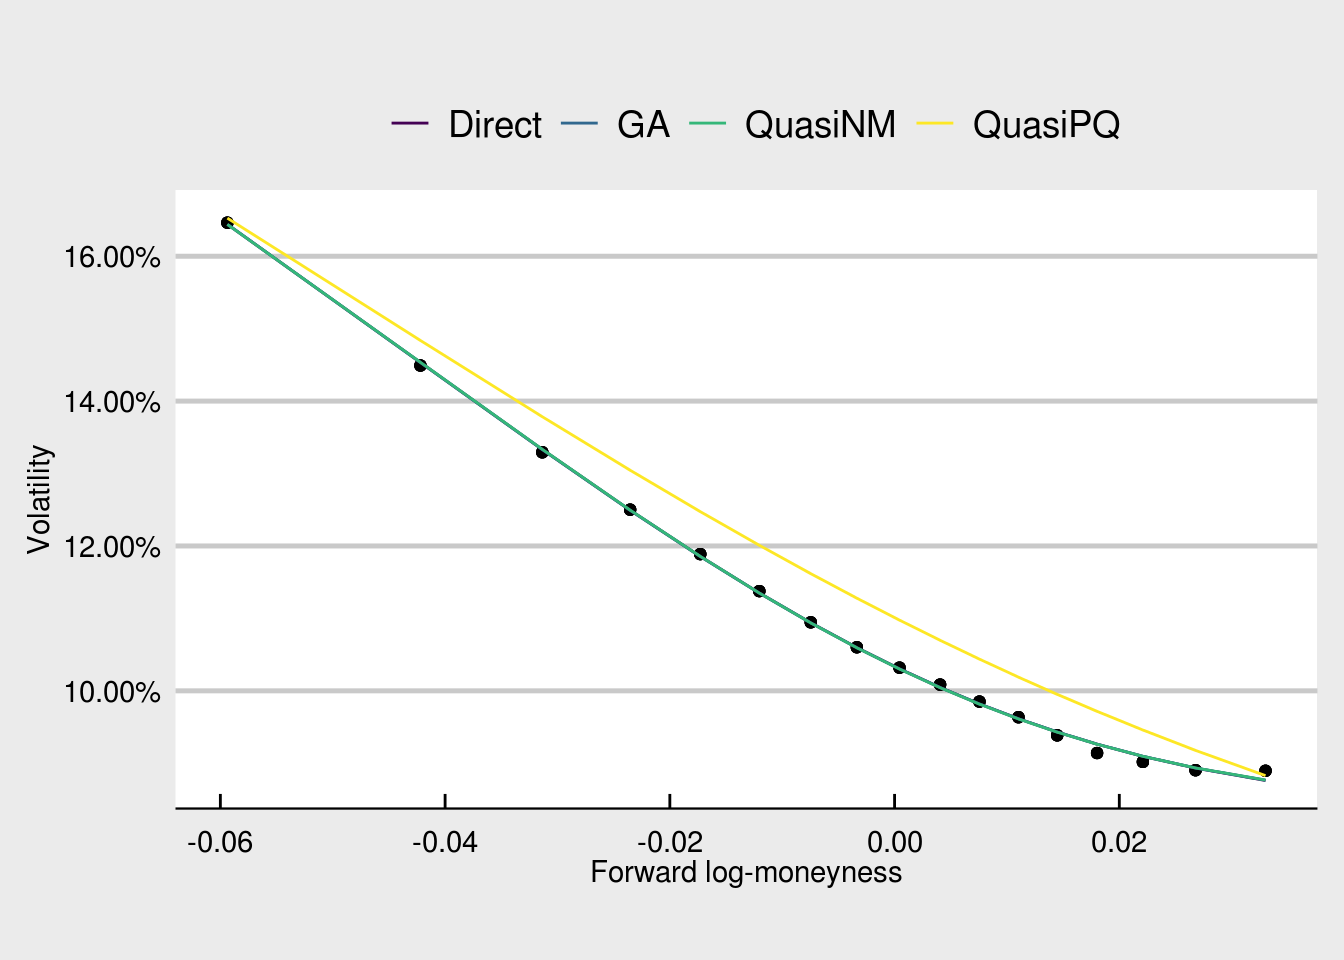
\includegraphics{07-calibrando-uma-svi_files/figure-latex/plot-1.pdf}
\caption{\label{fig:plot}Comparação entre diferentes métodos de calibração de uma
SVI.}
\end{figure}

De fato o método direto e o método \emph{Quasi-explicit} com otimizador
global do tipo algoritmo genético se mostram mais adequados para a
calibração de um SVI. Enquanto o método direto é muito mais eficiente em
termos computacionais, o método \emph{Quasi-explicit} com GA é mais
robusto. Desta forma, deve-se salientar que é necessário que o usuário,
ao fazer uma calibração de \emph{smile} de volatilidade, deve dispor de
diferentes métodos de fazê-lo, e a inspeção visual do resultado é
\textbf{obrigatória} para determinar qual método foi mais eficiente em
ajustar a curva aos dados.

\section{Conclusão}\label{conclusao-3}

Apesar de neste exemplo ter se mostrado um método efetivo, com bom
ajuste e baixo tempo de calibração, o método direto é altamente
dependente dos valores iniciais dos parâmetros. Para tornar este método
mais robusto, um número maior de reinicializações deve ser feita o que
penaliza o tempo de calibração. O método \emph{Quasi-explicit} com
algoritmo genético para encontrar a região de \((m, \sigma)\) onde se
encontra o mínimo global se mostrou bastante robusta, entretanto, de
convergência lenta. Para ajustar apenas um \emph{smile} alguns segundos
a mais não representam problema. Porém, se imaginarmos que em uma grande
instituição financeira são necessárias calibrações de, talvez, milhares
de \emph{smiles} representando inúmeras superfícies de diversos
instrumentos, este método pode se mostrar computacionalmente caro.

Já os métodos \emph{Quasi-explicit} que utilizam um algoritmo de
Nelder-Mead para a resolução do problema completo se mostraram muito
sensíveis às estimativas iniciais dos parâmetros. Mesmo utilizando 50
reinicialzações do método, diversas vezes o ajuste realizado foi
insatisfatório. A resolução através de programação quadrática é rápida,
se comparada com NM, entretanto, quando as restrições impostas pela
equação \eqref{eq:D} se tornam ativas, este método parece sofrer com algum
viés em sua solução.

\chapter{Superfície SVI}\label{ssvi}

Superfície SVI, ou somente SSVI é uma generalização do modelo
\protect\hyperlink{svi}{SVI} de \citep{Gatheral2004} que busca
solucionar o problema de restrição dos parâmetros do modelo para evitar
a presença de arbitragem do tipo borboleta em um dado \emph{smile}. Este
modelo foi proposto por \citep{Gatheral2014} e extende o modelo SVI
original apresentando duas outras parametrizações equivalentes e então o
modelo para superfícies propriamente dito.

\section{Reparametrizações
equivalentes}\label{reparametrizacoes-equivalentes}

Existem duas outras formas de se apresentar um modelo SVI que são
equivalentes a parametrização
\protect\hyperlink{superficies}{\emph{RAW}} já apresentada. Estas são as
parametrizações ``Natural'' e ``Jump-Wings'' que são apresentadas
abaixo.

Para um dado conjunto de parâmetros
\(\chi_N=\{\Delta, \mu, \rho, \omega, \zeta\}\) a parametrização natural
de um SVI é dada por:

\begin{equation}
w(k; \chi_N)=\Delta+\frac{\omega}{2}\left\lbrace 1+\zeta\rho(k-\mu)+\sqrt{(\zeta(k-\mu)+\rho)^2+(1-\rho^2)} \right\rbrace
\label{eq:svi-natural}
\end{equation}

onde \(\omega\geq 0\), \(\Delta, \mu \in \mathbb R\), \(|\rho|<1\) e
\(\zeta>0\). A correspondência entre as parametrizações \emph{raw} e
natural é dada pelo seguinte mapeamento e seu inverso:

\begin{equation}
(a, b, \rho, m, \sigma)=\left(\Delta+\frac{\omega}{2}(1-\rho^2), \frac{\omega\zeta}{2}, \rho, \mu-\frac{\rho}{\zeta}, \frac{\sqrt{1-\rho^2}}{\zeta}\right)
\label{eq:natural-to-raw}
\end{equation}

\begin{equation}
(\Delta, \mu, \rho, \omega, \zeta)=\left(a-\frac{\omega}{2}(1-\rho^2), m+\frac{\rho\sigma}{\sqrt{1-\rho^2}}, \rho, \frac{2b\sigma}{\sqrt{1-\rho^2}}, \frac{\sqrt{1-\rho^2}}{\sigma}\right)
\label{eq:raw-to-natural}
\end{equation}

A desvantagem destas parametrizações é que o valor de seus parâmetros
não são intuitivos para os \emph{traders}, eles não carregam estes
valores em sua memória durante a negociação. Valores característicos de
uma superfície de volatilidade implícita que \emph{traders} têm em mente
são, por exemplo, volatilidade ATM, \emph{skew} de volatilidade ATM e
assíntotas. Desta forma a parametrização \emph{Jump-Wings} é útil, pois
relaciona estes valores típicos aos parâmetros \emph{raw} de um SVI.

A parametrização \emph{JW} é dada em termos da variância implícita (e
não da variância total) e portanto existe uma dependência explícita do
tempo em sua formulação. Para um dado tempo até a expiração, \(\tau\), o
conjunto de parâmetros
\(\chi_{J}=\{v_\tau, \psi_\tau, p_\tau, c_\tau, \tilde v_\tau\}\) é
definido pelas seguintes equações a partir dos parâmetros \emph{raw}:

\begin{align}
v_\tau&=\frac{a+b\{-\rho m + \sqrt{m^2+\sigma^2}\}}{\tau},\\
\psi_\tau&=\frac{1}{\sqrt{w_\tau}}\frac{b}{2}\left(-\frac{m}{\sqrt{m^2+\sigma^2}}+\rho\right),\\
p_\tau&=\frac{1}{\sqrt{w_\tau}}b(1-\rho),\\
c_\tau&=\frac{1}{\sqrt{w_\tau}}b(1+\rho),\\
\tilde v_\tau&=\frac{1}{\tau}\left(a+b\sigma\sqrt{1-\rho^2}\right)
\label{eq:raw-to-jw}
\end{align}

onde \(w_\tau=v_\tau \tau\) relaciona a variância total ATM com a
variância ATM. Os parâmetros possuem as seguintes interpretações:
\(v_\tau\) é a variância ATM, \(\psi_\tau\) o \emph{skew} ATM,
\(p_\tau\) a inclinação da asa esquerda (puts), \(c_\tau\) a inclinação
da asa direita (calls) e \(\tilde v_\tau\) é a variância implícita
mínima.

A figura \ref{fig:svi-jw} apresenta uma esquematização destes parâmetros
sobre um \emph{smile} fictício para melhor compreensão.

\begin{figure}
\centering
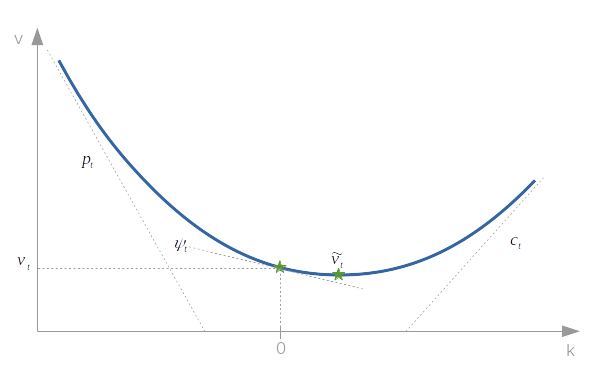
\includegraphics{./images/svi_jw.png}
\caption{\label{fig:svi-jw}Interpretação dos parâmetros de um SVI-JW.}
\end{figure}

As relações inversas que trazem uma parametrização \emph{JW} para uma
\emph{raw}, assumindo que \(m \neq 0\) são:

\begin{align}
b&=\frac{\sqrt{w_\tau}}{2}(c_\tau+p_\tau),\\
\rho&=1-\frac{p_\tau\sqrt{w_\tau}}{b},\\
a&=\tilde v_\tau \tau-b\sigma\sqrt{1-\rho^2},\\
m&=\frac{(v_\tau-\tilde v_\tau)\tau}{b\left\lbrace-\rho+sign(\alpha)\sqrt{1+\alpha^2}-\alpha\sqrt{1-\rho^2}\right\rbrace},\\
\sigma&=\alpha m.
\label{eq:jw-to-raw}
\end{align}

onde as variáveis auxiliares são definidas da seguinte forma:
\(\beta:=\rho-(2\psi_\tau\sqrt{w_\tau})/b\) e
\(\alpha:=sign(\beta)\sqrt{1/\beta^2 - 1}\), com \(\beta \in [-1, 1]\)
para garantir a convexidade do \emph{smile}.

Se \(m=0\), então as equações para \(a, b, \rho\) se mantêm, porém,
\(\sigma = (v_\tau \tau-a)/b\). Desta forma temos relações entre as três
parametrizações SVI, sendo possível navegar entre elas com
tranquilidade. Um \emph{trader} pode verificar no mercado os valores dos
parâmetros \emph{JW} e traduzi-los para \emph{raw} e simular o
\emph{smile} ou fazer o caminho reverso, calibrar uma fatia da
superfície com parâmetros \emph{raw}, traduzi-los para \emph{JW} e
apresentar para sua mesa, onde todos conseguirão interpretar os valores
a que estão habituados.

\section{Superfície SVI}\label{superficie-svi}

Uma SSVI surge como uma extensão à parametrização natural de um SVI, e
fornece em uma única equação, a possibilidade de parametrizar uma
superfície de volatilidade implícita por inteiro. É necessário, antes de
mais nada, fazer algumas definições preliminares. Defina a variância
total implícita no dinheiro (ATM) como
\(\theta_\tau:=\sigma_{BS}^2(0, \tau)\tau\) e
\(\lim\limits_{\tau\rightarrow 0}\theta_\tau = 0\).

\BeginKnitrBlock{definition}
\protect\hypertarget{def:ssvi}{}{\label{def:ssvi} }Seja \(\varphi\) uma
função suave em \(\mathbb R_+^*\mapsto \mathbb R_+^*\) tal que
\(\lim\limits_{\tau\rightarrow 0}\theta_\tau \varphi(\theta_\tau)\)
exista em \(\mathbb R\). Uma SSVI é definida por:
\EndKnitrBlock{definition}

\begin{equation}
w(k, \theta_\tau)=\frac{\theta_\tau}{2}\left\lbrace 1+\rho\varphi(\theta_\tau)k+\sqrt{(\varphi(\theta_\tau)k+\rho)^2+(1-\rho^2)} \right\rbrace
\label{eq:ssvi}
\end{equation}

Veja que na representação SSVI, engenhosamente os autores substituíram a
dimensão de tempo, \(\tau\), típica de superfícies de volatilidde, pela
variância total ATM. Com esta representação, eles conseguiram derivar as
condições necessárias para a ausência de arbitragem estática na
superfície e sempre que necessário, é possível retornar a dimensão de
tempo no calendário.

Agora é necessário definir a função \(\varphi\), que então será
substituída na equação \eqref{eq:ssvi} da definição \ref{def:ssvi} com
seus próprios parâmetros e teremos por fim uma função
\(w(k, \theta_\tau; \chi_{ssvi})\) que poderá ser calibrada para o
conjunto de parâmetros da SSVI, \(\chi_{ssvi}\) contra os dados
observados no mercado. No fundo, qualquer função que obedeça as
condições impostas na definição \ref{def:ssvi} pode ser utilizada,
entretanto os autores apresentam dois tipos de função que condizem com
as observações empíricas.

\subsection{Heston}\label{heston-1}

Considere a função \(\varphi\) definida por:

\begin{equation}
\varphi(\theta)\equiv\frac{1}{\gamma\theta}\left\lbrace 1-\frac{1-e^{-\gamma\theta}}{\gamma\theta}\right\rbrace
\label{eq:heston-phi}
\end{equation}

com \(\gamma > 0\). Esta função recebeu este nome pois, seu \emph{skew}
na variância implícita é compatível com aquele previsto no modelo de
\protect\hyperlink{superficies}{Heston}.

\subsection{Lei de potência}\label{lei-de-potencia}

A parametrização da função \(\varphi\) como uma lei de potência é
primeiramente considerada da seguinte forma:
\(\varphi(\theta)=\eta\theta^{-\gamma}\) com \(\eta > 0\) e
\(0<\gamma<1\). Entretanto, esta parametrização apresenta algumas
limitações com relação a arbitragem do tipo borboleta e então é proposta
a seguinte forma funcional:

\begin{equation}
\varphi(\theta)=\frac{\eta}{\theta^\gamma(1+\theta)^{1-\gamma}}
\label{eq:pl-phi}
\end{equation}

que é \textbf{garantida} não possuir arbitragem estática dado que
\(\eta(1+|\rho|)\leq 2\).

\section{Condições de não-arbitragem}\label{condicoes-de-nao-arbitragem}

As condições para ausência de arbitragem estática para uma SSVI são
colocadas através de dois teoremas (4.1 e 4.2) e provadas no artigo de
\citep{Gatheral2014}, dos quais resulta o seguinte corolário.

\BeginKnitrBlock{corollary}
\protect\hypertarget{cor:ssvi-arbitrage}{}{\label{cor:ssvi-arbitrage} }A
superfície SVI definida em \ref{def:ssvi} está livre de arbitragem
estática se as seguintes condições são satisfeitas:
\EndKnitrBlock{corollary}

\begin{enumerate}
\def\labelenumi{\arabic{enumi}.}
\tightlist
\item
  \(\partial_\tau\theta_\tau\geq 0, \text{ para todo } \tau > 0\)
\item
  \(0\leq \partial_\theta(\theta\varphi(\theta))\leq\frac{1}{\rho^2}\left(1+\sqrt{1-\rho^2}\right)\varphi(\theta), \text{ para todo } \theta>0\)
\item
  \(\theta\varphi(\theta)(1+|\rho|)<4, \text{ para todo } \theta>0\)
\item
  \(\theta\varphi(\theta)^2(1+|\rho|)\leq 4, \text{ para todo } \theta>0\)
\end{enumerate}

Onde os dois primeiros itens dizem respeito a ausência de arbitragem de
calendário, enquanto que os seguintes são exigências para a superfície
estar livre de arbitragem do tipo borboleta.

Para uma função \(\varphi\) do tipo Heston, as condições nos seus
parâmetros são: \(\gamma>0\) que garante o atendimentos as condições 1 e
2 do corolário \ref{cor:ssvi-arbitrage} e \(\gamma\geq(1+|\rho|)/4\)
para garantir a ausência de arbitragem borboleta, a qual subsume a
primeira condição.

Para a função do tipo lei de potência dada em \eqref{eq:pl-phi} são
necessárias as condições \(0<\gamma<1\) e \(\eta(1+|\rho|)\leq 2\)

A maneira típica de impor as restrições dos parâmetros no momento da
calibração do modelo é inserir uma penalidade na função objetivo, quando
a restrição é violada. Por exemplo, consideramos a restrição de
inequalidade para a lei de potência, \(\eta(1+|\rho|)-2\leq 0\). No
momento da calibração, nós devemos calcular o valor desta expressão e se
o seu resultado for maior que zero, uma penalidade é somada a função
objetivo da calibração (em geral a soma dos quadrados dos erros).

\section{Densidade neutra ao risco}\label{densidade-neutra-ao-risco}

Já comentamos sobre a \protect\hyperlink{rnd}{distribuição neutra ao
risco} implícita no preço de opções que pode ser obtida através da
fórmula de \citep{Breeden1978}, assim como já foi introduzida uma certa
função \protect\hyperlink{svi}{\(g(k)\)} que desempenha um papel
fundamental para garantir a ausência de arbitragem do tipo borboleta em
\emph{smiles} de variância total. O fato é que, para garantir a ausência
de arbitragem a função \(g(k)\) deve ser não negativa em todo o seu
suporte \(k \in \mathbb R\). Ao mesmo tempo, a definição de ausência de
arbitragem borboleta se confunde com o fato que a densidade neutra ao
risco deve também ser não negativa, caso contrário não seria uma
densidade de probabilidade. Logo percebe-se a estreita relação entre a
função \(g(k)\) e a densidade neutra ao risco implícita no preço de
opções. De fato, a fórmula de Breeden-Litzenberger nos fornece:

\begin{equation}
p(k)=\left.\frac{\partial^2C_B(k, w(k))}{\partial K^2}\right|_{K=Fe^k} 
\end{equation}

que após fazer as derivações da equação de Black e as substituições e
manipulações algébricas com as reparametrizações do modelo B\&S, resulta
em:

\begin{equation}
p(k)=\frac{g(k)}{\sqrt{2\pi w(k)}}\exp\left(-\frac{d_2(k)^2}{2}\right)
\label{eq:pk}
\end{equation}

E para relembrarmos, a função \(g(k)\) é dada por:

\begin{equation}
g(k)=\left(1-\frac{kw\prime(k)}{2w(k)}\right)^2-\frac{w\prime(k)^2}{4}\left(\frac{1}{w(k)}+\frac{1}{4}\right)+\frac{w\prime\prime(k)}{2}
\label{eq:g}
\end{equation}

Ou seja, uma vez parametrizado um SVI para um dado prazo de maturidade,
\(\tau\), se torna simples a tarefa de extrair a densidade implícita.
Possuímos a função \(w(k)\) e suas derivadas e certamente \(d_2(k)\),
bastando portanto, aplicar a equação \eqref{eq:pk} para extrair importante
informação do mercado de opções.

\section{Superfície de volatilidade
local}\label{superficie-de-volatilidade-local}

De maneira semelhante ao procedimento realizado com a densidade
implícita, também é possível, uma vez parametrizada a SSVI, derivar a
\textbf{superfície de volatilidade local} através da
\protect\hyperlink{superficies}{equação} de \citep{Dupire1994}. Esta
equação toma a seguinte forma funcional:

\begin{equation}
\sigma_L^2(K, \tau)=\frac{\partial_\tau C_B(K, \tau)}{\frac{1}{2}K^2\partial_{KK}C_B(K, \tau)}
\label{eq:dupire}
\end{equation}

Novamente tomando as derivadas da equação de Black e fazendo as
substituições necessárias\footnote{Referimos o leitor ao material do
  prof. Antoine Jacquier para uma prova desta relação
  \href{http://wwwf.imperial.ac.uk/~ajacquie/IC_AMDP/IC_AMDP_Docs/AMDP.pdf}{aqui}}
chegamos a relação entre a superfície SVI e variância local.

\begin{equation}
\sigma^2_L(k, \tau)=\frac{\partial_\tau w(k, \theta_\tau)}{g(k, w(k, \theta_\tau))}
\label{eq:var-local}
\end{equation}

De forma bastante simplista, a superfície de volatilidade local pode ser
entendida como aquela superfície de volatilidades instantâneas para o
ativo subjacente, \(\sigma(S, t)\) que depende tanto do nível de preço
deste ativo quanto do tempo, e fornece a previsão do mercado para a
volatilidade instantânea de \(S\) dado que este ativo hoje está
precificado em \(S_0\) e no tempo futuro \(\tau\) estará em \(K\).
Fazendo uma analogia com o mercado de juros, a superfície local está
para a curva \emph{forward} assim como a superfície implícita está para
a curva de juros, numa aproximação.

A superfície local é muito utilizada para precificar opções exóticas,
aquelas que possuem perfil de \emph{payoff} distinto das opções
europeias e podem ou não terem seus resultados atrelados ao caminho
seguido pelo preço do ativo objeto durante a vida da opção. Nestes
casos, a precificação se dá através da incorporação da superfície local
estipulando um valor de volatilidade instantânea para cada possível
combinação \((S_t, t)\) em geral em um ambiente de simulação de
\protect\hyperlink{monte-carlo}{Monte Carlo}.

No caso da equação \eqref{eq:var-local} temos uma nova derivada a ser
computada, \(\partial_\tau w(k, \theta_\tau)\), que só poderia ser feita
de forma analítica caso \(\theta_\tau\) fosse parametrizada
explicitamente. Nem sempre este é o caso, já que \(\theta_\tau\) são os
valores de variância total ATM implícitas, ou seja, observa-se no
mercado apenas alguns \textbf{pontos} de \(\theta_\tau\), pontos estes
que podem estar espaçados em intervalos diferentes de tempo. A solução
para esta derivação é interpolar estes pontos, nem que seja uma simples
interpolação linear, e então fazer a derivação de forma numérica através
de um método de diferenças finitas. Note que na interpolação deve-se
garantir a condição de não arbitragem de calendário,
\(\partial_\tau\theta_\tau\geq 0\).

\section{Calibração da SSVI}\label{calibracao-da-ssvi}

Vamos retomar nosso exemplo de superfície de volatilidade do
\protect\hyperlink{svi}{artigo anterior}, porém agora com todas as datas
de expiração, ou seja, a superfície completa. Os códigos
\href{https://cran.r-project.org/}{R} apresentados abaixo ajudam na
compreensão do procedimento.

\begin{Shaded}
\begin{Highlighting}[]
\KeywordTok{library}\NormalTok{(readr)}
\KeywordTok{library}\NormalTok{(dplyr)}
\KeywordTok{library}\NormalTok{(purrr)}
\KeywordTok{library}\NormalTok{(kableExtra)}
\KeywordTok{library}\NormalTok{(ggplot2)}
\KeywordTok{library}\NormalTok{(ggthemes)}
\KeywordTok{library}\NormalTok{(plot3D)}
\KeywordTok{source}\NormalTok{(}\StringTok{'svi.R'}\NormalTok{)}
\KeywordTok{source}\NormalTok{(}\StringTok{'ssvi.R'}\NormalTok{)}
\end{Highlighting}
\end{Shaded}

Primeiramente foram carregados os pacotes necessários para a leitura e
manipulação dos dados (\texttt{readr}, \texttt{dplyr} e \texttt{purrr})
assim como os pacotes de visualização (\texttt{kableExtra},
\texttt{ggplot2}, \texttt{ggthemes} e \texttt{plot3D}). Em seguida os
arquivos \texttt{svi.R} e \texttt{ssvi.R} são implementações do
\href{http://clubedefinancas.com.br/}{Clube de Finanças} para as funções
necessárias para calibrar uma SSVI.

Carregados os pacotes e as funções, deve-se carregar os dados da
superfície de volatilidade e organizá-los da forma que necessitamos.

\begin{Shaded}
\begin{Highlighting}[]
\NormalTok{ssvi_data <-}\StringTok{ }\KeywordTok{read_csv}\NormalTok{(}\StringTok{"./R/input/IV_Raw_Delta_surface.csv"}\NormalTok{,}
                     \DataTypeTok{col_types =} \KeywordTok{cols}\NormalTok{(}\DataTypeTok{date =} \KeywordTok{col_date}\NormalTok{(}\DataTypeTok{format =} \StringTok{"%m/%d/%Y"}\NormalTok{))) }\OperatorTok\StringTok{ }
\StringTok{  }\KeywordTok{mutate}\NormalTok{(}\DataTypeTok{tau =}\NormalTok{ period }\OperatorTok{/}\StringTok{ }\DecValTok{365}\NormalTok{,}
         \DataTypeTok{theta =} \KeywordTok{theta_vec}\NormalTok{(moneyness, tau, iv)) }\OperatorTok\StringTok{ }
\StringTok{  }\KeywordTok{rename}\NormalTok{(}\DataTypeTok{k =}\NormalTok{ moneyness)}
\end{Highlighting}
\end{Shaded}

Para calibrar os parâmetros de uma SSVI, com a função \(\varphi\) do
tipo \textbf{lei de potência}, necessitaremos dos dados de
\emph{moneyness} (\(k\)), vencimento (\(\tau\)) e volatilidade implícita
(\(iv\)) que será internamente convertida em variância total implícita
(\(w\)). Dentro da função de ajuste dos parâmetros \texttt{fit\_ssvi()}
a variância total ATM implícita \(\theta_\tau\) é calculada através de
interpolação \emph{spline} para cada uma das fatias da superfície, pois,
nossos dados não necessariamente possuem esta observação. Cabe ressaltar
também que os dados estão organizados de forma \texttt{tidy}, sendo
portanto, todos os argumentos passados para as funções na forma de
vetores, não sendo necessário gerar uma matriz contendo o \emph{grid}
\((k, \tau)\).

\begin{Shaded}
\begin{Highlighting}[]
\NormalTok{k <-}\StringTok{ }\NormalTok{ssvi_data}\OperatorTok{$}\NormalTok{k}
\NormalTok{tau <-}\StringTok{ }\NormalTok{ssvi_data}\OperatorTok{$}\NormalTok{tau}
\NormalTok{iv <-}\StringTok{ }\NormalTok{ssvi_data}\OperatorTok{$}\NormalTok{iv}
\NormalTok{theta <-}\StringTok{ }\NormalTok{ssvi_data}\OperatorTok{$}\NormalTok{theta}

\KeywordTok{set.seed}\NormalTok{(}\DecValTok{12345}\NormalTok{)}
\NormalTok{powerlaw_par <-}\StringTok{ }\KeywordTok{fit_ssvi}\NormalTok{(tau, k, iv, }\StringTok{"powerlaw"}\NormalTok{)}
\KeywordTok{kable}\NormalTok{(powerlaw_par,}
      \DataTypeTok{caption =} \StringTok{"Parâmetros da SSVI-power-law estimados."}\NormalTok{,}
      \DataTypeTok{col.names =} \StringTok{"SSVI-PL"}\NormalTok{)}
\end{Highlighting}
\end{Shaded}

\begin{table}[t]

\caption{\label{tab:ssvi-cal}Parâmetros da SSVI-power-law estimados.}
\centering
\begin{tabular}{l|r}
\hline
  & SSVI-PL\\
\hline
rho & -0.6479238\\
\hline
gamma & 0.4926757\\
\hline
eta & 0.8607807\\
\hline
\end{tabular}
\end{table}

Podemos rapidamente checar se estes parâmetros estimados geram uma
superfície livre de arbitragem.

\begin{Shaded}
\begin{Highlighting}[]
\KeywordTok{paste}\NormalTok{(}\StringTok{"Parametrização livre de arbitragem borboleta? :"}\NormalTok{, }
      \KeywordTok{ssvi_butterfly_cons}\NormalTok{(powerlaw_par, }\StringTok{"powerlaw"}\NormalTok{) }\OperatorTok{<=}\StringTok{ }\DecValTok{0}\NormalTok{)}
\end{Highlighting}
\end{Shaded}

\begin{verbatim}
## [1] "Parametrização livre de arbitragem borboleta? : TRUE"
\end{verbatim}

Com os parâmetros estimados, é simples plotar todos os \emph{smiles} que
compõe a superfície e verificar visualmente o ajuste. Vamos plotar a
\textbf{variância total} em função do \emph{moneyness} e vencimentos,
pois neste gráfico se verifica a condição de arbitragem de calendário
simplesmente através do fato que as curvas geradas não devem se cruzar.

\begin{Shaded}
\begin{Highlighting}[]
\NormalTok{plt_df <-}\StringTok{ }\NormalTok{ssvi_data }\OperatorTok\StringTok{ }
\StringTok{  }\KeywordTok{mutate}\NormalTok{(}\DataTypeTok{w_pl =} \KeywordTok{ssvi_fun}\NormalTok{(powerlaw_par, theta, k)) }\OperatorTok\StringTok{ }
\StringTok{  }\KeywordTok{select}\NormalTok{(k, tau, w_pl, iv) }\OperatorTok\StringTok{ }
\StringTok{  }\KeywordTok{filter}\NormalTok{(tau }\OperatorTok{<}\StringTok{ }\FloatTok{0.5}\NormalTok{)}

\KeywordTok{ggplot}\NormalTok{(plt_df, }\KeywordTok{aes}\NormalTok{(}\DataTypeTok{x =}\NormalTok{ k, }\DataTypeTok{y =}\NormalTok{ w_pl)) }\OperatorTok{+}\StringTok{ }
\StringTok{  }\KeywordTok{geom_line}\NormalTok{(}\KeywordTok{aes}\NormalTok{(}\DataTypeTok{color =} \KeywordTok{as.factor}\NormalTok{(}\KeywordTok{format}\NormalTok{(tau, }\DataTypeTok{digits =} \DecValTok{3}\NormalTok{)))) }\OperatorTok{+}
\StringTok{  }\KeywordTok{geom_point}\NormalTok{(}\KeywordTok{aes}\NormalTok{(}\DataTypeTok{y =}\NormalTok{ iv}\OperatorTok{^}\DecValTok{2} \OperatorTok{*}\StringTok{ }\NormalTok{tau)) }\OperatorTok{+}
\StringTok{  }\KeywordTok{guides}\NormalTok{(}\DataTypeTok{color =} \KeywordTok{guide_legend}\NormalTok{(}\DataTypeTok{title =} \StringTok{"Vencimento"}\NormalTok{)) }\OperatorTok{+}
\StringTok{  }\KeywordTok{labs}\NormalTok{(}\DataTypeTok{title =} \StringTok{"SSVI Lei de Potência",}
\StringTok{       x = "}\NormalTok{Forward log}\OperatorTok{-}\KeywordTok{moneyness}\NormalTok{ (k)}\StringTok{",}
\StringTok{       y = "}\NormalTok{Variância total implí}\KeywordTok{cita}\NormalTok{ (w)}\StringTok{",}
\StringTok{       caption = "}\NormalTok{Elaborado por Rafael Bressan para o Clube de Finanças.}\StringTok{") +}
\StringTok{#  scale_y_continuous(labels = scales::percent) +}
\StringTok{  scale_color_viridis_d() +}
\StringTok{  theme_economist_white()}
\end{Highlighting}
\end{Shaded}

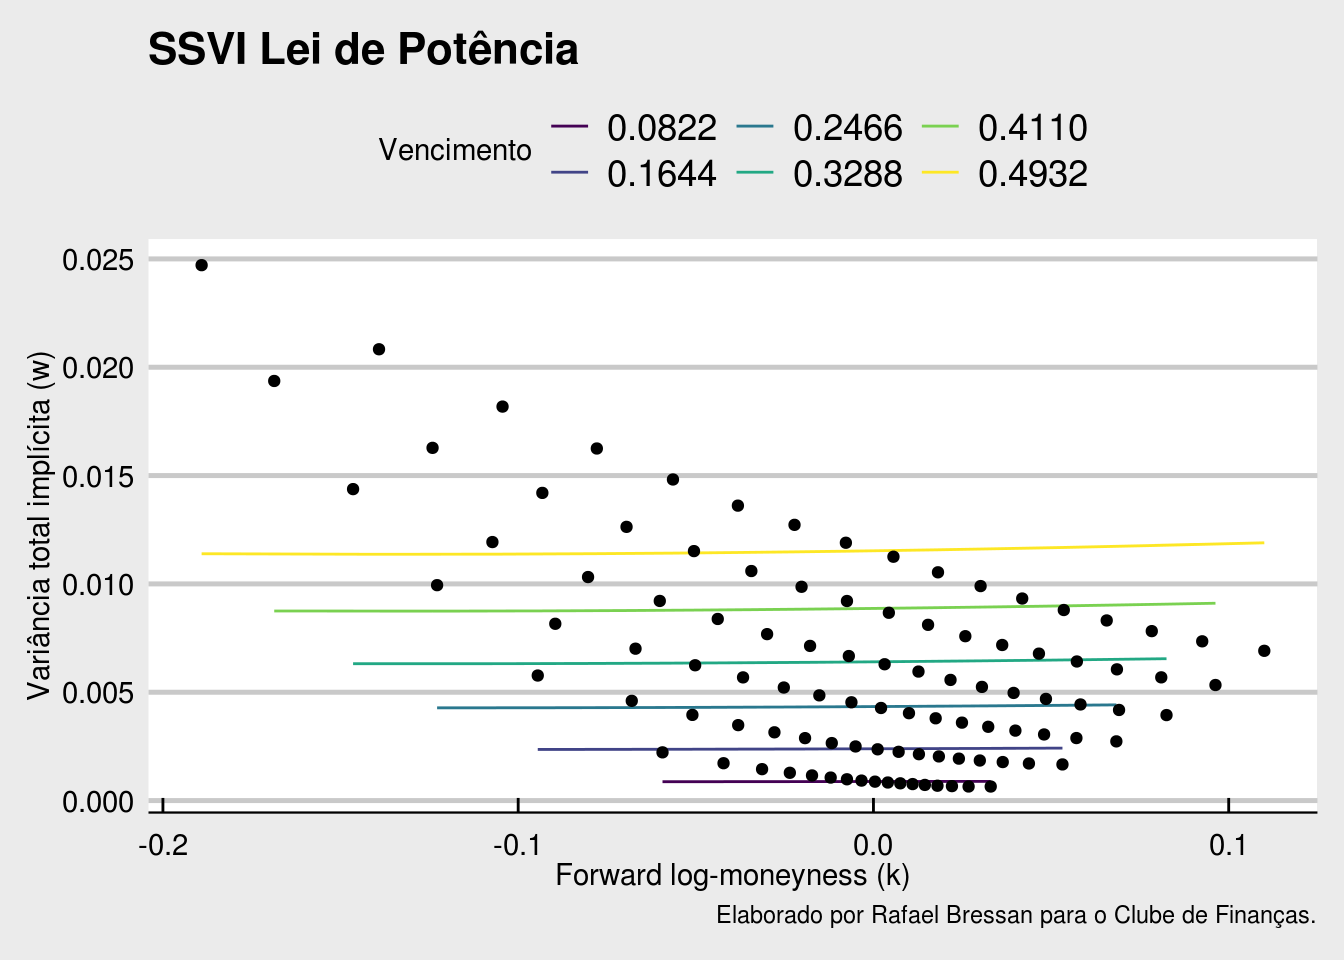
\includegraphics{08-superficie-svi_files/figure-latex/ssvi_plot-1.pdf}

Foram retirados os vencimentos mais longos apenas para uma melhor
visualização da parte mais curta da superfície, que em geral é a mais
complicada de se calibrar através de SVI. O resultado parece
interessante, com as variâncias ao redor do dinheiro tendo boa aderência
aos dados observados, porém para \emph{puts} muito fora do dinheiro, a
parametrização aparenta \textbf{subestimar} o valor da variância total e
portanto estaria subprecificando as opções.

Iremos agora verificar a \emph{densidade da distribuição implícita} para
o período de vencimento de 90 dias. Utiliza-se para tanto a equação
\eqref{eq:pk} onde \(w(k)\) (e suas derivadas e o próprio \(d_2\)) será
agora calculado com base nos parâmetros da tabela \ref{tab:ssvi-cal}
para um vetor de \emph{moneyness} mais amplo e denso. O resultado pode
ser observado através da figura \ref{fig:ssvi-dens}

\begin{Shaded}
\begin{Highlighting}[]
\NormalTok{thetadens <-}\StringTok{ }\NormalTok{ssvi_data }\OperatorTok\StringTok{ }
\StringTok{  }\KeywordTok{filter}\NormalTok{(period }\OperatorTok{==}\StringTok{ }\DecValTok{90}\NormalTok{) }\OperatorTok\StringTok{ }
\StringTok{  }\KeywordTok{pull}\NormalTok{(theta) }\OperatorTok\StringTok{ }
\StringTok{  `}\DataTypeTok{[}\StringTok{`}\NormalTok{(}\DecValTok{1}\NormalTok{)}
\NormalTok{kdens <-}\StringTok{ }\KeywordTok{seq}\NormalTok{(}\OperatorTok{-}\FloatTok{0.5}\NormalTok{, }\FloatTok{0.3}\NormalTok{, }\DataTypeTok{length.out =} \DecValTok{100}\NormalTok{)}
\NormalTok{dens <-}\StringTok{ }\KeywordTok{ssvi_density}\NormalTok{(powerlaw_par, thetadens, kdens, }\StringTok{"powerlaw"}\NormalTok{)}
\NormalTok{dens_tbl <-}\StringTok{ }\KeywordTok{tibble}\NormalTok{(}\DataTypeTok{kdens =}\NormalTok{ kdens, }\DataTypeTok{dens =}\NormalTok{ dens)}

\KeywordTok{ggplot}\NormalTok{(dens_tbl, }\KeywordTok{aes}\NormalTok{(}\DataTypeTok{x =}\NormalTok{ kdens, }\DataTypeTok{y =}\NormalTok{ dens)) }\OperatorTok{+}\StringTok{ }
\StringTok{  }\KeywordTok{geom_line}\NormalTok{() }\OperatorTok{+}
\StringTok{  }\KeywordTok{labs}\NormalTok{(}\DataTypeTok{title =} \StringTok{"Densidade neutra ao risco SSVI"}\NormalTok{,}
     \DataTypeTok{x =} \StringTok{"Forward log-moneyness (k)"}\NormalTok{,}
     \DataTypeTok{y =} \StringTok{"Densidade"}\NormalTok{,}
     \DataTypeTok{caption =} \StringTok{"Elaborado por Rafael Bressan para o Clube de Finanças."}\NormalTok{) }\OperatorTok{+}
\StringTok{  }\KeywordTok{scale_color_viridis_d}\NormalTok{() }\OperatorTok{+}
\StringTok{  }\KeywordTok{theme_economist_white}\NormalTok{()}
\end{Highlighting}
\end{Shaded}

\begin{figure}
\centering
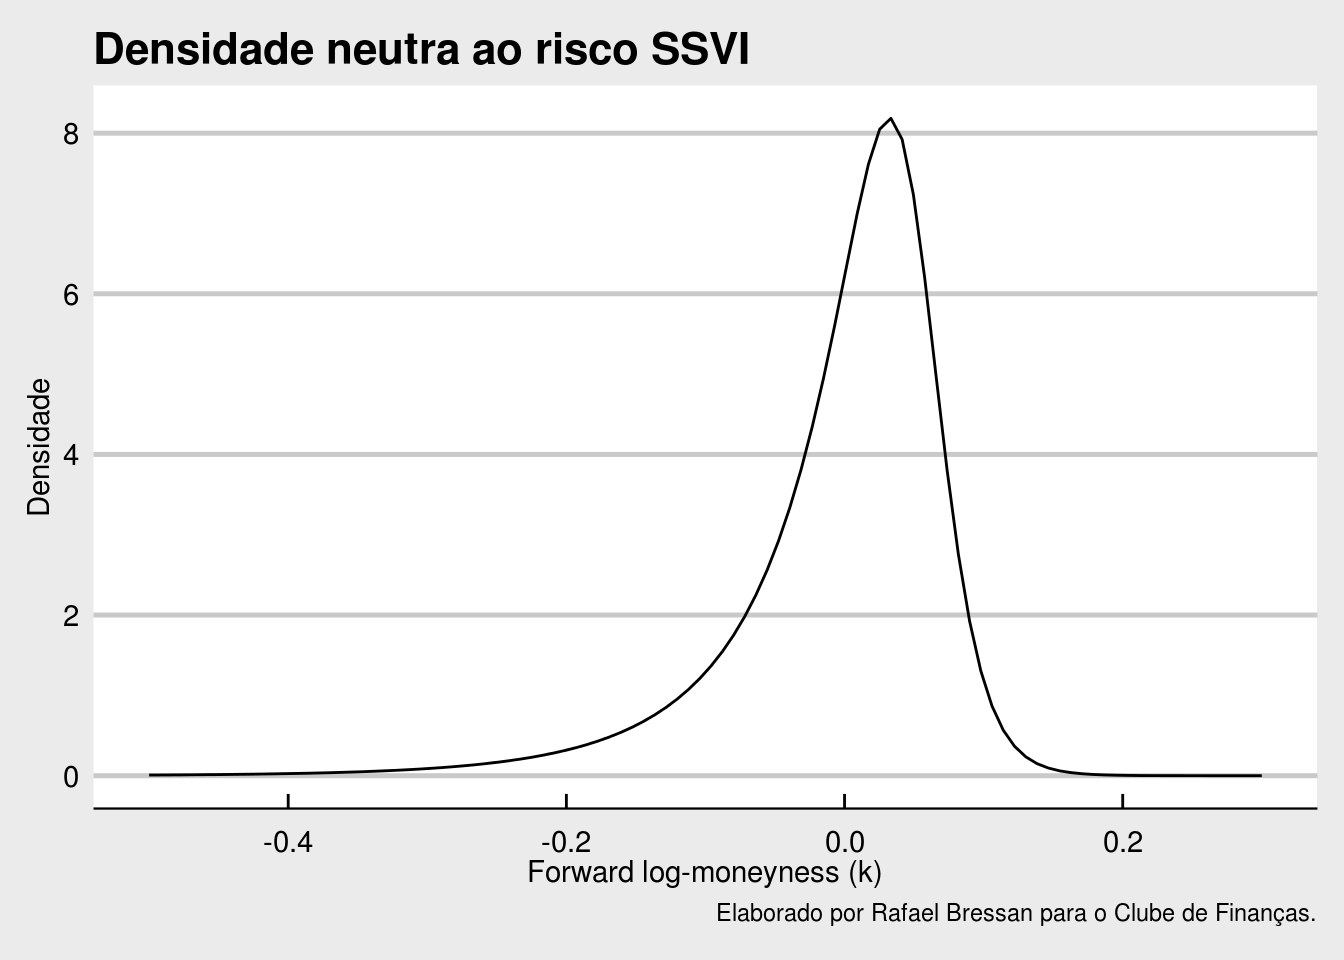
\includegraphics{08-superficie-svi_files/figure-latex/ssvi-dens-1.pdf}
\caption{\label{fig:ssvi-dens}Densidade implícita estimada. Presença de
assimetria e leptocurtose a esquerda.}
\end{figure}

Este é um gráfico interessante, que nos mostra exatamente o que se
espera de um \emph{smile} típico de \emph{equities} que possui
\emph{skew} negativo. Percebemos como a densidade de probabilidades é
assimétrica, com a cauda esquerda muito mais longa, refletindo o
sentimento de mercado de uma maior probabilidade de grandes quedas no
preço do ativo objeto que altas equivalentes. Sempre que verificamos um
\emph{smile} com \emph{skew} negativo, como é o presente caso, a
distribuição de probabilidades é assimétrica a esquerda.

Vamos conferir se a área sob esta curva de densidade integra
aproximadamente 1, como deve ser.

\begin{Shaded}
\begin{Highlighting}[]
\NormalTok{area <-}\StringTok{ }\KeywordTok{integrate}\NormalTok{(}\ControlFlowTok{function}\NormalTok{(x) }\KeywordTok{ssvi_density}\NormalTok{(powerlaw_par, thetadens, x, }\StringTok{"powerlaw"}\NormalTok{),}
                  \DataTypeTok{lower =}\NormalTok{ kdens[}\DecValTok{1}\NormalTok{],}
                  \DataTypeTok{upper =}\NormalTok{ kdens[}\KeywordTok{length}\NormalTok{(kdens)])}
\KeywordTok{paste}\NormalTok{(}\StringTok{"Área sob a curva de densidade é: "}\NormalTok{, area}\OperatorTok{$}\NormalTok{value)}
\end{Highlighting}
\end{Shaded}

{[}1{]} ``Área sob a curva de densidade é: 0.999302879362191''

Chegou o momento de inferirmos a \textbf{superfície de volatilidade
local} a partir de nossa parametrização SSVI. O método será a aplicação
direta da equação \eqref{eq:var-local} pois, com a parametrização
realizada, dispomos de todos os dados necessários para seu cômputo.

Antes porém, devemos observar uma peculiaridade dos nossos dados. O site
\href{https://ivolatility.com}{ivolatility.com} fornece dados alinhados
por \textbf{Delta}, ou seja, para cada período de vencimento temos um
mesmo conjunto de Deltas, \textbf{mas não de moneyness}. Os valores
deste último irá variar conforme o vencimento, uma vez que pela
definição de \emph{forward log-moneyness} que vimos utilizando é
dependente do tempo para maturidade da opção. Desta forma precisamos
gerar um novo \emph{grid} \((k, \tau)\) para plotar nossa superfície de
volatilidade local.

Para tanto, criaremos uma sequência uniforme de valores de \(k\) e
tomaremos os valores que já possuímos de \(\tau\) e \(\theta_\tau\)
recombinando-os através da função \texttt{expand.grid()} para gerar o
data frame que precisamos.

Feito isso, é apenas questão de aplicar a equação \eqref{eq:var-local} e
criar uma matriz (pois assim pede a função \texttt{surf3D()}) com os
valores da volatilidade local.

\begin{Shaded}
\begin{Highlighting}[]
\NormalTok{kloc <-}\StringTok{ }\KeywordTok{seq}\NormalTok{(}\OperatorTok{-}\NormalTok{.}\DecValTok{4}\NormalTok{, }\FloatTok{0.4}\NormalTok{, }\DataTypeTok{length.out =} \DecValTok{17}\NormalTok{)}
\NormalTok{utau <-}\StringTok{ }\KeywordTok{unique}\NormalTok{(tau)}
\NormalTok{utheta <-}\StringTok{ }\KeywordTok{unique}\NormalTok{(theta)}
\KeywordTok{names}\NormalTok{(utheta) <-}\StringTok{ }\NormalTok{utau  }\CommentTok{# utheta will be a lookup vector}
\NormalTok{grid_df <-}\StringTok{ }\KeywordTok{expand.grid}\NormalTok{(kloc, utau) }\OperatorTok\StringTok{ }
\StringTok{  }\KeywordTok{rename}\NormalTok{(}\DataTypeTok{kloc =}\NormalTok{ Var1,}
         \DataTypeTok{tau =}\NormalTok{ Var2) }\OperatorTok\StringTok{ }
\StringTok{  }\KeywordTok{mutate}\NormalTok{(}\DataTypeTok{theta =}\NormalTok{ utheta[}\KeywordTok{as.character}\NormalTok{(tau)])}

\NormalTok{loc_vol_vec <-}\StringTok{ }\KeywordTok{ssvi_local_vol}\NormalTok{(powerlaw_par, }
\NormalTok{                              grid_df}\OperatorTok{$}\NormalTok{tau, }
\NormalTok{                              grid_df}\OperatorTok{$}\NormalTok{theta, }
\NormalTok{                              grid_df}\OperatorTok{$}\NormalTok{kloc, }
                              \StringTok{"powerlaw"}\NormalTok{)}
\CommentTok{# Matrix where k is row}
\NormalTok{loc_vol_m <-}\StringTok{ }\KeywordTok{matrix}\NormalTok{(loc_vol_vec, }\DataTypeTok{nrow =} \KeywordTok{length}\NormalTok{(kloc))  }

\CommentTok{# Plot Local Volatility Surface}
\CommentTok{# x is k, y is tau}
\NormalTok{M <-}\StringTok{ }\KeywordTok{mesh}\NormalTok{(kloc, utau)}
\KeywordTok{surf3D}\NormalTok{(M}\OperatorTok{$}\NormalTok{x, M}\OperatorTok{$}\NormalTok{y, loc_vol_m, }\DataTypeTok{colkey =} \OtherTok{FALSE}\NormalTok{, }\DataTypeTok{bty =} \StringTok{"b2"}\NormalTok{, }
       \DataTypeTok{phi =} \DecValTok{20}\NormalTok{, }\DataTypeTok{ticktype =} \StringTok{"detailed"}\NormalTok{,}
       \DataTypeTok{xlab =} \StringTok{"k"}\NormalTok{,}
       \DataTypeTok{ylab =} \StringTok{"\textbackslash{}u03c4"}\NormalTok{,}
       \DataTypeTok{zlab =} \StringTok{"Volatilidade local \textbackslash{}u03c3"}\NormalTok{)}
\end{Highlighting}
\end{Shaded}

\begin{verbatim}
## Warning in persp.default(plist$xlim, plist$ylim, z = matrix(nrow = 2, ncol
## = 2, : conversion failure on 'τ' in 'mbcsToSbcs': dot substituted for <cf>
\end{verbatim}

\begin{verbatim}
## Warning in persp.default(plist$xlim, plist$ylim, z = matrix(nrow = 2, ncol
## = 2, : conversion failure on 'τ' in 'mbcsToSbcs': dot substituted for <84>
\end{verbatim}

\begin{verbatim}
## Warning in persp.default(plist$xlim, plist$ylim, z = matrix(nrow = 2, ncol
## = 2, : conversion failure on 'Volatilidade local σ' in 'mbcsToSbcs': dot
## substituted for <cf>
\end{verbatim}

\begin{verbatim}
## Warning in persp.default(plist$xlim, plist$ylim, z = matrix(nrow = 2, ncol
## = 2, : conversion failure on 'Volatilidade local σ' in 'mbcsToSbcs': dot
## substituted for <83>
\end{verbatim}

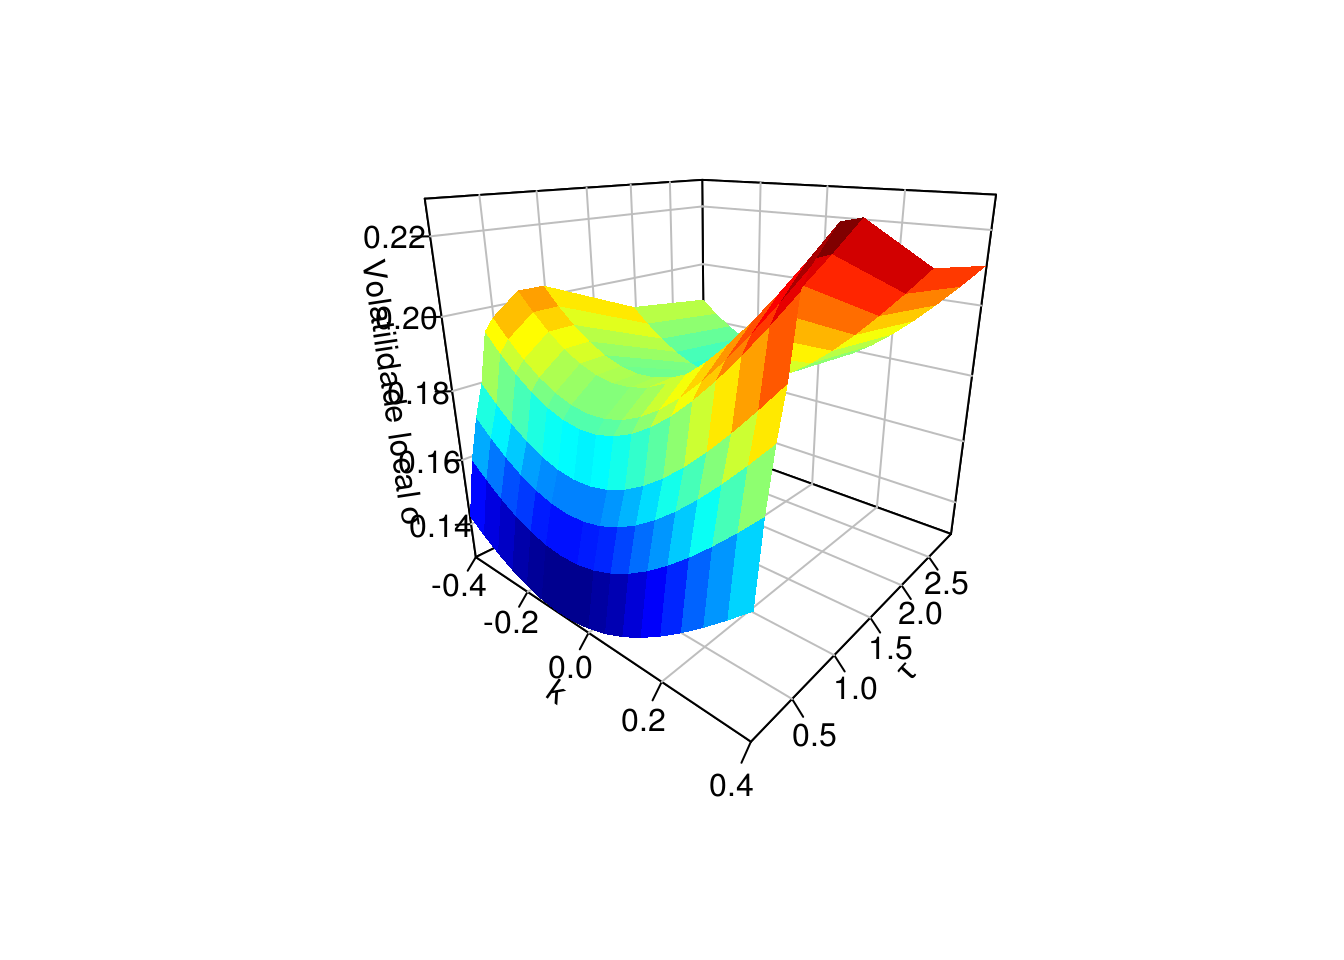
\includegraphics{08-superficie-svi_files/figure-latex/vol-local-1.pdf}

\section{Conclusão}\label{conclusao-4}

Apresentamos o modelo de superfícies SVI, que faz uma generalização dos
\emph{smiles} SVI e apresenta vantagens sobre a parametrização
fatia-a-fatia em virtude dos teoremas sobre arbitragem estática,
apresentando restrições para os parâmetros do modelo que garantem a
ausência deste tipo de arbitragem.

Uma vez parametrizada toda uma SSVI, torna-se simples, uma mera
aplicação de fórmulas a obtenção tanto da densidade da distribuição
neutra ao risco implícita no preços das opções, como da superfície de
volatilidade local através da equação de Dupire.

\section{Referências}\label{referencias-1}

\hypertarget{monte-carlo}{\chapter{Simulação de Monte
Carlo}\label{monte-carlo}}

Em capítulo anterior, sobre
\protect\hyperlink{processos-estocasticos}{processos estocásticos},
fizemos uso de uma poderosa ferramenta computacional, frequentemente
utilizada em finanças para fazer simulações. Naquele artigo simulamos
cinco realizações de caminhos de um processo estocástico, cada um com
500 passos a frente. Esta técnica é conhecida como Simulação de Monte
Carlo - SMC e será abordada no presente artigo.

Neste artigo também iremos introduzir, no corpo do texto, os códigos em
linguagem \href{https://cran.r-project.org/}{R} utilizados para fazer as
simulações, aumentando a didática de nossos artigos. A linguagem R é uma
das preferidas para a modelagem estatística, é uma das linguagens de
ciência de dados que vem ganhando muitos adeptos e, por conseguinte, é
amplamente utilizada pelo mercado financeiro. E claro, é uma das
preferidas aqui do CF também.

Nosso problema será simular a posição de um portfólio composto por uma
posição comprada em uma ação \texttt{PETR4} e uma \emph{put}
\texttt{PETRV17}. A opção de venda (\emph{put}) tem preço de exercício
em R\$ 16,92, data de expiração em 15/10/2018 e é do tipo europeia. Ao
final do pregão do dia 21/09/2018 a ação \texttt{PETR4} fechou cotada a
R\$ 20,14 e a \emph{put} em R\$ 0,12. A partir desta data até o dia da
expiração da opção haverão 16 dias de pregão, que será nosso horizonte
de simulação.

Para melhoria da didática do texto e também para simplificação do
problema, manteremos algumas variáveis necessárias para a precificação
de opções constantes ao longo do período de análise, são elas:

\begin{itemize}
\item
  Volatilidade: Será calculada a volatilidade implícita da opção da data
  de compra do portfólio, 21/09/2018, e será mantida constante a partir
  daí para fins de precificação na SMC;
\item
  Taxa de juros: constante no valor de 6,5 \%a.a. tem termos contínuos;
\item
  Taxa de dividendos: suposto igual a zero.
\end{itemize}

\section{Simulação de Monte Carlo}\label{simulacao-de-monte-carlo}

Para realizar uma SMC de um ativo financeiro deve-se primeiramente
estabelecer uma distribuição de probabilidades que os retornos deste
ativo deve seguir. Em nosso exemplo, utilizaremos a distrbuição normal
para os retornos logarítimicos da ação \texttt{PETR4}, em linha com o
clássico modelo \emph{Black \& Scholes}, certamente existem diversas
variantes que se ajustam melhor a realidade dos mercados, entretanto
este é o modelo mais conhecido e base de todos os demais.

Uma vez escolhida a distribuição dos (log) retornos, tem-se de escolher
valores para a média e variância desta distribuição. A média dos
retornos iremos tirar do histórico da ação, o retorno médio diário dos
último ano. A variância da distribuição será encontrada a partir da
volatilidade implícita da opção na data de compra do portfólio. A função
utilizada para encontrar esta volatilidade retorna um valor em termos
anuais, portanto, conforme visto no capítulo sobre
\protect\hyperlink{processos-estocasticos}{processos estocásticos}
devemos reescalar uma volatilidade anual para diária, e isto é obtido
fazendo a divisão por \(\sqrt{252}\), onde temos 252 dias úteis em 1
ano.

Desta forma é possível fazer a simulação dos log-retornos da ação para
cada um dos dias a frente, até a data de exercício da opção, 15/10/2018.
Estes retornos são acumulados e o preço \textbf{simulado} da ação
\texttt{PETR4} em uma data intermediária é o preço de compra vezes o
retorno acumulado até então.

Faremos 1.000 simulações destas, gerando caminhos possíveis de preços
para a ação. É necessário fazer muitas simulações para termos uma boa
ideia da distribuição dos preços na data final, não é raro serem feitas
mais de mil simulações, as vezes até dez mil podem ser necessárias.

Uma vez gerados todos os caminhos simulados do preço do ativo objeto,
podemos então precificar a \emph{put} com base nestes preços simulados e
as outras variáveis necessárias para se precificar uma opção europeia.
Assim teremos também todos os caminhos de preço para a opção até sua
data de exercício.

O valor de nosso portfólio, em qualquer ponto do intervalo de tempo em
análise, será a soma do preço da ação com o preço da opção e será
possível verificar o efeito de proteção contra quedas do preço do ativo
objeto a compra da \emph{put} tem no portfólio.

Cabe ressaltar aqui que o preço da opção \textbf{não} é simulado, não
diretamente. Como a opção é um instrumento derivativo o seu preço
``deriva'' do preço do ativo objeto, este sim que é simulado. Uma vez
que tenhamos o preço da ação, dadas nossas premissas de precificação,
podemos calcular o prêmio da opção com base no modelo \emph{Black \&
Scholes}.

\section{Implementação em R}\label{implementacao-em-r}

Conforme comentado, utilizamos aqui no CF a linguagem de programação
\href{https://cran.r-project.org/}{R} para realizar nossas atividades
que envolvam métodos quantitativos em finanças. Abaixo irei apresentar o
código utilizado, trecho a trecho e o resultado obtido ao final.

Primeiramente, no R, devemos carregar em nossa sessão de trabalho os
pacotes que serão utilizados ao longo do código. Os pacotes funcionam
como extensões ao R base, nestes pacotes encontramos diversas funções já
programadas por outras pessoas que facilitam (e muito!) a nossa
codificação.

\begin{Shaded}
\begin{Highlighting}[]
\KeywordTok{library}\NormalTok{(tidyverse)}
\KeywordTok{library}\NormalTok{(ggthemes)}
\KeywordTok{library}\NormalTok{(tidyquant)}
\KeywordTok{library}\NormalTok{(ragtop)}
\end{Highlighting}
\end{Shaded}

O pacote \texttt{ragtop}, por exemplo, possui já implementado dentro
dele funções para fazer a precificação de opções europeias, sem que se
tenha que implementar o modelo manualmente. Como a intenção deste artigo
não é explicar o modelo \emph{Black \& Scholes}, vamos abstrair esta
parte e simplesmente chamar uma função que nos retorna o valor da opção
dadas as variáveis de entrada.

Em seguida iremos definir algumas de nossas variáveis, como o
\emph{ticker} da ação para buscar seus dados históricos através da
função \texttt{tq\_get()} do pacote \texttt{tidyquant} e calcular os
retornos logarítimicos e tirar sua média, o preço e data de exercício da
opção e também iremos relacionar os dias entre a data de compra e
vencimento.

\begin{Shaded}
\begin{Highlighting}[]
\NormalTok{acao <-}\StringTok{ "PETR4.SA"}
\NormalTok{p_exer <-}\StringTok{ }\FloatTok{16.92}
\NormalTok{d_exer <-}\StringTok{ }\KeywordTok{as.Date}\NormalTok{(}\StringTok{"2018-10-15"}\NormalTok{)}
\NormalTok{d_atual <-}\StringTok{ }\KeywordTok{as.Date}\NormalTok{(}\StringTok{"2018-09-21"}\NormalTok{)}
\NormalTok{dias <-}\StringTok{ }\KeywordTok{seq}\NormalTok{(d_atual, d_exer, }\DataTypeTok{by =} \DecValTok{1}\NormalTok{)}
\CommentTok{#dias <- dias[isBusinessDay("Brazil", dias)]}
\NormalTok{nsims <-}\StringTok{ }\DecValTok{1000}
\NormalTok{ndias <-}\StringTok{ }\KeywordTok{length}\NormalTok{(dias) }\OperatorTok{-}\StringTok{ }\DecValTok{1}
\NormalTok{sim_nomes <-}\StringTok{ }\KeywordTok{paste0}\NormalTok{(}\StringTok{"sim"}\NormalTok{, }\DecValTok{1}\OperatorTok{:}\NormalTok{nsims)}

\CommentTok{# Carregar os precos historicos da acao}
\NormalTok{p_hist <-}\StringTok{ }\KeywordTok{tq_get}\NormalTok{(acao, }\DataTypeTok{from =}\NormalTok{ d_atual }\OperatorTok{-}\StringTok{ }\KeywordTok{years}\NormalTok{(}\DecValTok{1}\NormalTok{), }\DataTypeTok{to =}\NormalTok{ d_atual }\OperatorTok{+}\StringTok{ }\KeywordTok{days}\NormalTok{(}\DecValTok{1}\NormalTok{)) }\OperatorTok\StringTok{ }
\StringTok{  }\KeywordTok{filter}\NormalTok{(volume }\OperatorTok{!=}\StringTok{ }\FloatTok{0.0}\NormalTok{)}
\NormalTok{ret_hist <-}\StringTok{ }\NormalTok{p_hist }\OperatorTok\StringTok{ }
\StringTok{  }\KeywordTok{tq_mutate}\NormalTok{(}\DataTypeTok{select =}\NormalTok{ adjusted,}
            \DataTypeTok{mutate_fun =}\NormalTok{ periodReturn,}
            \DataTypeTok{period =} \StringTok{"daily"}\NormalTok{,}
            \DataTypeTok{type =} \StringTok{"log"}\NormalTok{,}
            \DataTypeTok{leading =} \OtherTok{FALSE}\NormalTok{,}
            \DataTypeTok{col_rename =} \StringTok{"log_ret"}\NormalTok{) }\OperatorTok\StringTok{ }
\StringTok{  }\KeywordTok{na.omit}\NormalTok{()}
\NormalTok{rf <-}\StringTok{ }\KeywordTok{log}\NormalTok{(}\DecValTok{1} \OperatorTok{+}\StringTok{ }\FloatTok{0.065}\NormalTok{)}
\NormalTok{div <-}\StringTok{ }\DecValTok{0}
\NormalTok{S0 <-}\StringTok{ }\KeywordTok{last}\NormalTok{(ret_hist}\OperatorTok{$}\NormalTok{adjusted)}
\NormalTok{P0 <-}\StringTok{ }\FloatTok{0.12}
\NormalTok{mi <-}\StringTok{ }\DecValTok{252} \OperatorTok{*}\StringTok{ }\KeywordTok{mean}\NormalTok{(ret_hist}\OperatorTok{$}\NormalTok{log_ret) }\CommentTok{# retorno medio em termos anuais}
\NormalTok{sigma <-}\StringTok{ }\KeywordTok{implied_volatility}\NormalTok{(P0, }\OperatorTok{-}\DecValTok{1}\NormalTok{, S0, p_exer, rf, (ndias }\OperatorTok{+}\StringTok{ }\DecValTok{1}\NormalTok{) }\OperatorTok{/}\StringTok{ }\DecValTok{365}\NormalTok{, }
                            \DataTypeTok{divrate =}\NormalTok{ div)}
\end{Highlighting}
\end{Shaded}

Com o código acima obtemos basicamente todos os dados com os quais
poderemos implementar a simulação de Monte Carlo. Entretanto, para
realizar as simulações, necessitamos especificar mais algumas funções
customizadas para nossas necessidades.

Primeiro iremos especificar uma função que retorna uma única simulação
de log-retornos acumulados em uma coluna de dados, esta função é chamada
de \texttt{mc\_sim\_fun}. A segunda função necessária é a função de
precificação da opção europeia. Por padrão, a função
\texttt{blackscholes()} do pacote \texttt{ragtop} retorna uma lista com
o valor da opção, mas também suas gregas \(\Delta\) e \(\nu\).

\begin{Shaded}
\begin{Highlighting}[]
\CommentTok{# Funcao para realizar uma simulacao}
\NormalTok{mc_sim_fun <-}\StringTok{ }\ControlFlowTok{function}\NormalTok{(valor_i, N, media, volat)\{}
\NormalTok{  med_d <-}\StringTok{ }\NormalTok{media }\OperatorTok{/}\StringTok{ }\DecValTok{252}
\NormalTok{  volat_d <-}\StringTok{ }\NormalTok{volat }\OperatorTok{/}\StringTok{ }\KeywordTok{sqrt}\NormalTok{(}\DecValTok{252}\NormalTok{)}
\NormalTok{  ans <-}\StringTok{ }\KeywordTok{tibble}\NormalTok{(}\KeywordTok{c}\NormalTok{(valor_i, }\KeywordTok{rnorm}\NormalTok{(N, med_d }\OperatorTok{-}\StringTok{ }\NormalTok{(volat_d}\OperatorTok{^}\DecValTok{2} \OperatorTok{/}\StringTok{ }\DecValTok{2}\NormalTok{), volat_d))) }\OperatorTok\StringTok{ }
\StringTok{    `}\DataTypeTok{colnames<-}\StringTok{`}\NormalTok{(}\StringTok{"log_ret"}\NormalTok{) }\OperatorTok
\StringTok{    }\KeywordTok{mutate}\NormalTok{(}\DataTypeTok{ret_ac =} \KeywordTok{cumsum}\NormalTok{(log_ret)) }\OperatorTok\StringTok{ }
\StringTok{    }\KeywordTok{select}\NormalTok{(ret_ac)}
  
  \KeywordTok{return}\NormalTok{(ans)}
\NormalTok{\}}

\CommentTok{# Funcao para precificar uma opcao europeia}
\NormalTok{eur_option <-}\StringTok{ }\ControlFlowTok{function}\NormalTok{(type, S0, K, r, time, vola, div) \{}
\NormalTok{  callput <-}\StringTok{ }\KeywordTok{ifelse}\NormalTok{(type }\OperatorTok{==}\StringTok{ "call"}\NormalTok{, }\DecValTok{1}\NormalTok{, }\OperatorTok{-}\DecValTok{1}\NormalTok{)}
  
\NormalTok{  ans <-}\StringTok{ }\KeywordTok{blackscholes}\NormalTok{(callput, S0, K, r, time, vola, }\DataTypeTok{divrate =}\NormalTok{ div)}\OperatorTok{$}\NormalTok{Price}
  \KeywordTok{return}\NormalTok{(ans)}
\NormalTok{\}}
\end{Highlighting}
\end{Shaded}

Uma vez com os dados obtidos e as funções auxiliares programadas,
podemos passar a SMC propriamente dita. Aqui vamos estabelecer o número
de simulações (1.000), calcular um \emph{data frame} com os log-retornos
acumulados e então calcular o preço da ação para cada dia e simulação
realizados. O preço da ação na data \(t\) será \(S_t=S_0 e^{r_t}\), onde
\(r_t\) é o log-retorno acumulado até a data \(t\).

Após termos todos os preços do ativo objeto, passamos a computar qual
seria o preço da opção, \(P_t\), naquelas condições. O valor do
portfólio é dado pela soma destes dois preços (lembre-se, nosso
portfólio é composto por \textbf{uma} ação e uma opção de venda).

\begin{Shaded}
\begin{Highlighting}[]
\CommentTok{# Simulacao de Monte Carlo}
\CommentTok{# Valores Iniciais}
\NormalTok{inic <-}\StringTok{ }\KeywordTok{rep}\NormalTok{(}\DecValTok{0}\NormalTok{, nsims) }
\KeywordTok{set.seed}\NormalTok{(}\DecValTok{12345}\NormalTok{)}
\NormalTok{ret_ac_mc <-}\StringTok{ }\KeywordTok{map_dfc}\NormalTok{(inic,}
\NormalTok{                     mc_sim_fun,}
                     \DataTypeTok{N =}\NormalTok{ ndias,}
                     \DataTypeTok{media =}\NormalTok{ mi,}
                     \DataTypeTok{volat =}\NormalTok{ sigma)}

\NormalTok{precos_acao <-}\StringTok{ }\NormalTok{(S0 }\OperatorTok{*}\StringTok{ }\KeywordTok{exp}\NormalTok{(ret_ac_mc)) }\OperatorTok\StringTok{ }
\StringTok{  }\KeywordTok{set_names}\NormalTok{(sim_nomes) }\OperatorTok\StringTok{ }
\StringTok{  }\KeywordTok{mutate}\NormalTok{(}\DataTypeTok{anos_exp =}\NormalTok{ (ndias}\OperatorTok{:}\DecValTok{0}\NormalTok{) }\OperatorTok{/}\StringTok{ }\DecValTok{252}\NormalTok{) }\OperatorTok\StringTok{ }
\StringTok{  }\KeywordTok{gather}\NormalTok{(}\DataTypeTok{key =}\NormalTok{ sims, }\DataTypeTok{value =}\NormalTok{ St, }\OperatorTok{-}\NormalTok{anos_exp)}

\CommentTok{# Evolucao do Portfolio}
\NormalTok{port_mc <-}\StringTok{ }\NormalTok{precos_acao }\OperatorTok\StringTok{ }
\StringTok{  }\KeywordTok{mutate}\NormalTok{(}\DataTypeTok{Pt =} \KeywordTok{map2_dbl}\NormalTok{(St, anos_exp, }
                       \OperatorTok{~}\KeywordTok{eur_option}\NormalTok{(}\DataTypeTok{type =} \StringTok{"put"}\NormalTok{,}
                                   \DataTypeTok{S0 =}\NormalTok{ .x,}
                                   \DataTypeTok{K =}\NormalTok{ p_exer,}
                                   \DataTypeTok{r =}\NormalTok{ rf,}
                                   \DataTypeTok{time =}\NormalTok{ .y,}
                                   \DataTypeTok{vola =}\NormalTok{ sigma,}
                                   \DataTypeTok{div =}\NormalTok{ div)),}
         \DataTypeTok{port_valor =}\NormalTok{ Pt }\OperatorTok{+}\StringTok{ }\NormalTok{St,}
         \DataTypeTok{data =} \KeywordTok{rep}\NormalTok{(dias, nsims))}
\KeywordTok{head}\NormalTok{(port_mc)}
\end{Highlighting}
\end{Shaded}

\begin{verbatim}
##     anos_exp sims       St         Pt port_valor       data
## 1 0.09523810 sim1 19.40838 0.19814037   19.60652 2018-09-21
## 2 0.09126984 sim1 19.74659 0.14627994   19.89287 2018-09-22
## 3 0.08730159 sim1 20.16159 0.09894207   20.26053 2018-09-23
## 4 0.08333333 sim1 20.11181 0.09428249   20.20610 2018-09-24
## 5 0.07936508 sim1 19.86686 0.10511830   19.97198 2018-09-25
## 6 0.07539683 sim1 20.22476 0.07026524   20.29503 2018-09-26
\end{verbatim}

O \emph{data frame} \texttt{port\_mc} contém todas as informações da SMC
de nosso portfólio. Contém as datas desde o dia da compra até a data de
vencimento da opção e contém \textbf{todos} os caminhos de \(S_t\),
\(P_t\) e do portfólio. Vamos plotar os resultados obtidos para a
evolução apenas da ação, primeiramente.

\begin{Shaded}
\begin{Highlighting}[]
\NormalTok{brk <-}\StringTok{ }\KeywordTok{round}\NormalTok{(}\KeywordTok{sort}\NormalTok{(}\KeywordTok{c}\NormalTok{(p_exer, }\KeywordTok{seq}\NormalTok{(}\KeywordTok{min}\NormalTok{(port_mc}\OperatorTok{$}\NormalTok{St),}
                                \KeywordTok{max}\NormalTok{(port_mc}\OperatorTok{$}\NormalTok{St),}
                                \DataTypeTok{length.out =} \DecValTok{5}\NormalTok{))),}
             \DataTypeTok{digits =} \DecValTok{2}\NormalTok{)}
\KeywordTok{ggplot}\NormalTok{(port_mc, }\KeywordTok{aes}\NormalTok{(}\DataTypeTok{x =}\NormalTok{ data, }\DataTypeTok{y =}\NormalTok{ St)) }\OperatorTok{+}\StringTok{ }
\StringTok{  }\KeywordTok{geom_line}\NormalTok{(}\KeywordTok{aes}\NormalTok{(}\DataTypeTok{color =}\NormalTok{ sims)) }\OperatorTok{+}
\StringTok{  }\KeywordTok{geom_hline}\NormalTok{(}\DataTypeTok{yintercept =}\NormalTok{ p_exer, }\DataTypeTok{color =} \StringTok{"red"}\NormalTok{) }\OperatorTok{+}
\StringTok{  }\KeywordTok{guides}\NormalTok{(}\DataTypeTok{color =} \OtherTok{FALSE}\NormalTok{) }\OperatorTok{+}
\StringTok{  }\KeywordTok{labs}\NormalTok{(}\DataTypeTok{title =} \StringTok{"Simulações do Valor da Ação"}\NormalTok{,}
       \DataTypeTok{x =} \StringTok{"data"}\NormalTok{,}
       \DataTypeTok{y =} \StringTok{"Valor (R$)"}\NormalTok{) }\OperatorTok{+}
\StringTok{  }\KeywordTok{scale_y_continuous}\NormalTok{(}\DataTypeTok{breaks =}\NormalTok{ brk) }\OperatorTok{+}
\StringTok{  }\KeywordTok{scale_x_date}\NormalTok{(}\DataTypeTok{date_breaks =} \StringTok{"2 days"}\NormalTok{, }\DataTypeTok{date_labels =} \StringTok{"%d"}\NormalTok{) }\OperatorTok{+}
\StringTok{  }\KeywordTok{scale_color_viridis_d}\NormalTok{() }\OperatorTok{+}
\StringTok{  }\KeywordTok{theme_economist_white}\NormalTok{()}
\end{Highlighting}
\end{Shaded}

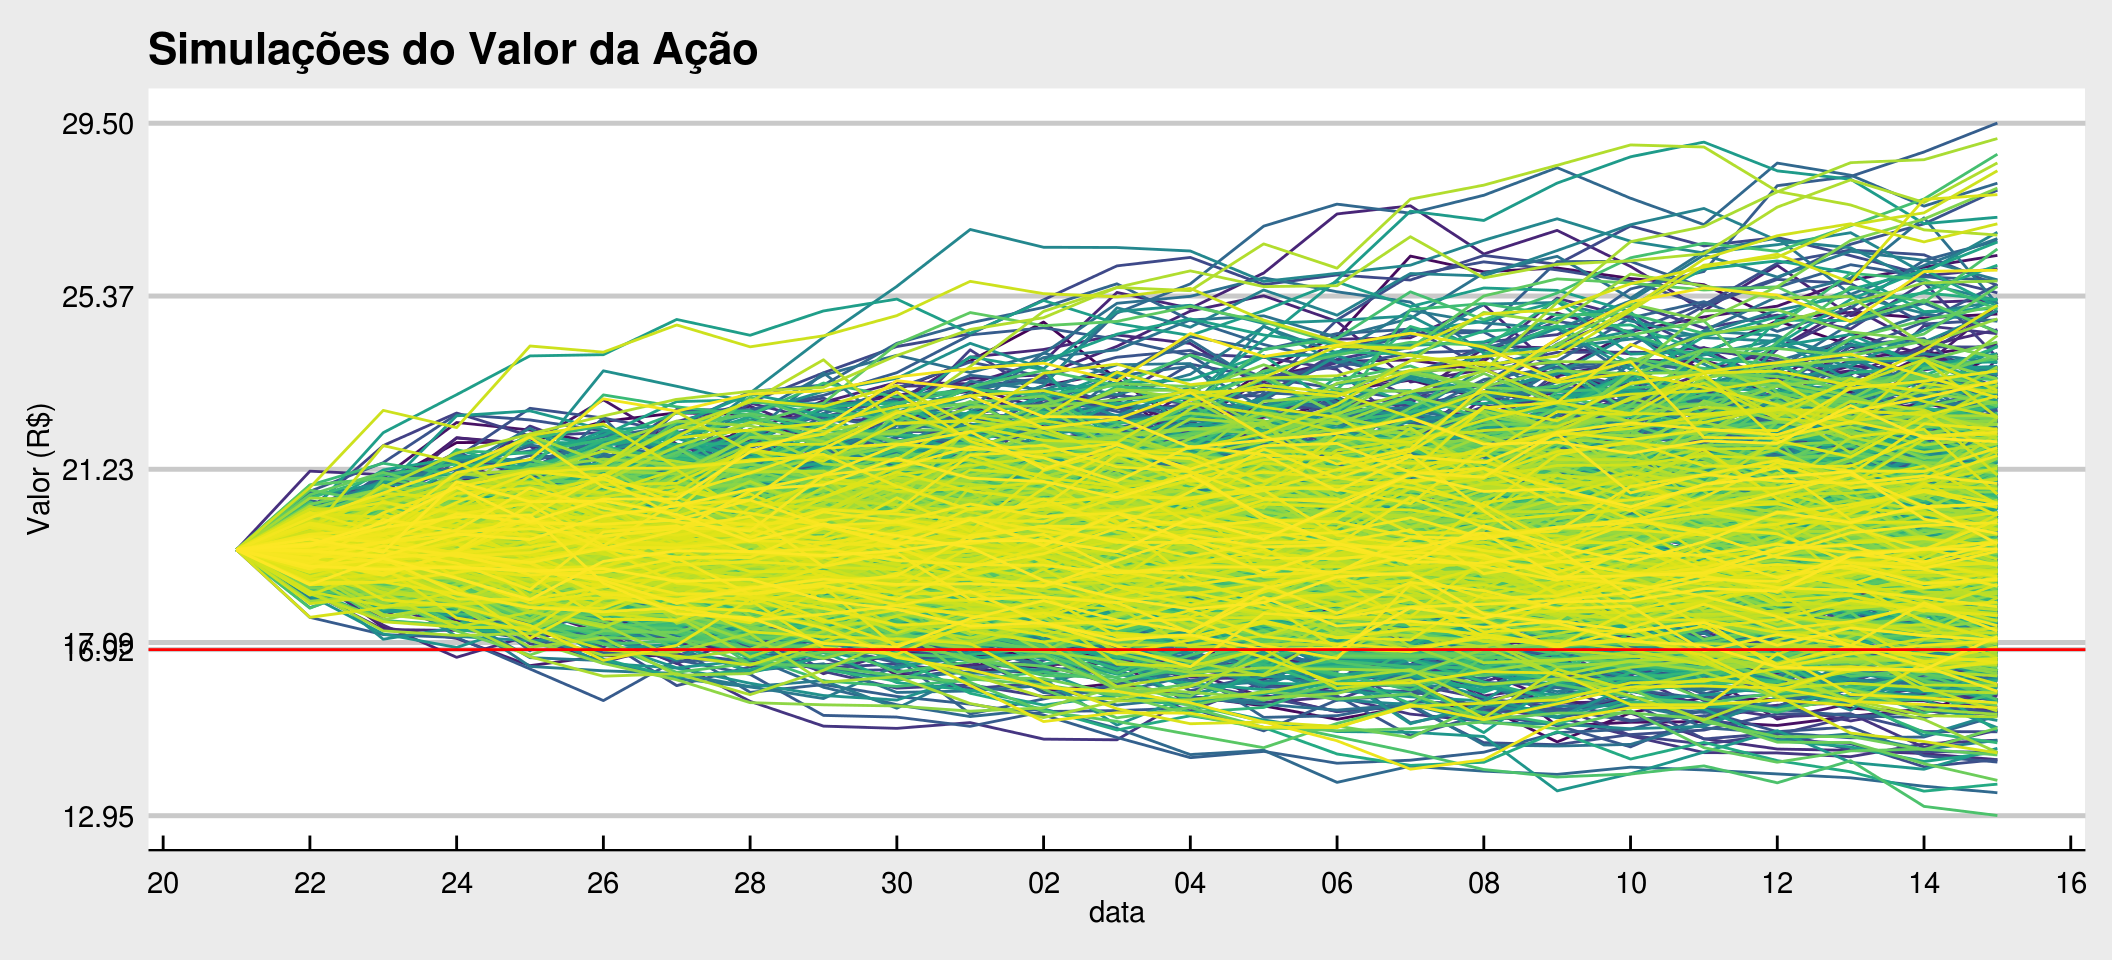
\includegraphics{91-monte-carlo_files/figure-latex/gr_acao-1.pdf}

Podemos verificar pela figura acima que a ação, pela nossa SMC, deve
fechar na maioria dos caminhos simulados acima do preço de exercício da
\emph{put} (linha vermelha). Entretanto existe uma menor probabilidade
de, até a data de vencimento, o preço da ação cair abaixo do
\emph{strike} desta opção.

Podemos inferir esta probabilidade através do número de caminhos que
terminaram em preço da ação abaixo do valor de referência. O custo de
proteção contra este risco é o prêmio por nós ao comprarmos a
\emph{put}. O código para esta inferência está abaixo.

\begin{Shaded}
\begin{Highlighting}[]
\NormalTok{p_baixo <-}\StringTok{ }\NormalTok{port_mc }\OperatorTok\StringTok{ }
\StringTok{  }\KeywordTok{filter}\NormalTok{(data }\OperatorTok{==}\StringTok{ }\NormalTok{d_exer) }\OperatorTok\StringTok{ }
\StringTok{  }\KeywordTok{summarise}\NormalTok{(}\DataTypeTok{num_baixo =} \KeywordTok{sum}\NormalTok{(St }\OperatorTok{<}\StringTok{ }\NormalTok{p_exer)) }\OperatorTok\StringTok{ }
\StringTok{  }\KeywordTok{as.double}\NormalTok{()}
\NormalTok{prob <-}\StringTok{ }\NormalTok{p_baixo }\OperatorTok{/}\StringTok{ }\NormalTok{nsims}
\end{Highlighting}
\end{Shaded}

Este cálculo nos mostra que em 134 caminhos simulados do preço de
\texttt{PETR4}, este terminou abaixo do preço de exercío da opção
\texttt{PETRV17}, ou seja, uma probabilidade de 13.4\%.

Para nos precavermos desta possível queda de preço e garantir um valor
mínimo de nosso portfólio até a data de 15/10/2018, podemos comprar uma
opção de venda, com preço de exercício no valor que desejamos e então o
portfólio passa a ser composto pela ação e também pela opção. Caso na
data de vencimento o preço da ação seja menor que o preço de exercício
da \emph{put}, esta opção estará ITM e pode ser exercida pelo valor da
diferença entre os preços, ou seja, nos garantindo que nosso portfólio
estará avaliado em R\$ 16,92.

Esta dinâmica pode ser verificada pela figura abaixo, que agora
apresenta o valor do portfólio completo, ação mais opção. Verificamos
que, de fato, no dia 15/10/2018 nosso investimento não estará em
situação pior que o preço garantido pela compra da \emph{put}.

\begin{Shaded}
\begin{Highlighting}[]
\NormalTok{brk <-}\StringTok{ }\KeywordTok{round}\NormalTok{(}\KeywordTok{sort}\NormalTok{(}\KeywordTok{c}\NormalTok{(p_exer, }\KeywordTok{seq}\NormalTok{(}\KeywordTok{min}\NormalTok{(port_mc}\OperatorTok{$}\NormalTok{port_valor),}
                                \KeywordTok{max}\NormalTok{(port_mc}\OperatorTok{$}\NormalTok{port_valor),}
                                \DataTypeTok{length.out =} \DecValTok{5}\NormalTok{)[}\OperatorTok{-}\DecValTok{1}\NormalTok{])),}
             \DataTypeTok{digits =} \DecValTok{2}\NormalTok{)}
\KeywordTok{ggplot}\NormalTok{(port_mc, }\KeywordTok{aes}\NormalTok{(}\DataTypeTok{x =}\NormalTok{ data, }\DataTypeTok{y =}\NormalTok{ port_valor)) }\OperatorTok{+}\StringTok{ }
\StringTok{  }\KeywordTok{geom_line}\NormalTok{(}\KeywordTok{aes}\NormalTok{(}\DataTypeTok{color =}\NormalTok{ sims)) }\OperatorTok{+}
\StringTok{  }\KeywordTok{geom_hline}\NormalTok{(}\DataTypeTok{yintercept =}\NormalTok{ p_exer, }\DataTypeTok{color =} \StringTok{"red"}\NormalTok{) }\OperatorTok{+}
\StringTok{  }\KeywordTok{guides}\NormalTok{(}\DataTypeTok{color =} \OtherTok{FALSE}\NormalTok{) }\OperatorTok{+}
\StringTok{  }\KeywordTok{labs}\NormalTok{(}\DataTypeTok{title =} \StringTok{"Simulações do Valor do Portfolio"}\NormalTok{,}
       \DataTypeTok{x =} \StringTok{"data"}\NormalTok{,}
       \DataTypeTok{y =} \StringTok{"Valor (R$)"}\NormalTok{) }\OperatorTok{+}
\StringTok{  }\KeywordTok{scale_y_continuous}\NormalTok{(}\DataTypeTok{breaks =}\NormalTok{ brk) }\OperatorTok{+}
\StringTok{  }\KeywordTok{scale_x_date}\NormalTok{(}\DataTypeTok{date_breaks =} \StringTok{"2 days"}\NormalTok{, }\DataTypeTok{date_labels =} \StringTok{"%d"}\NormalTok{) }\OperatorTok{+}
\StringTok{  }\KeywordTok{scale_color_viridis_d}\NormalTok{() }\OperatorTok{+}
\StringTok{  }\KeywordTok{theme_economist_white}\NormalTok{()}
\end{Highlighting}
\end{Shaded}

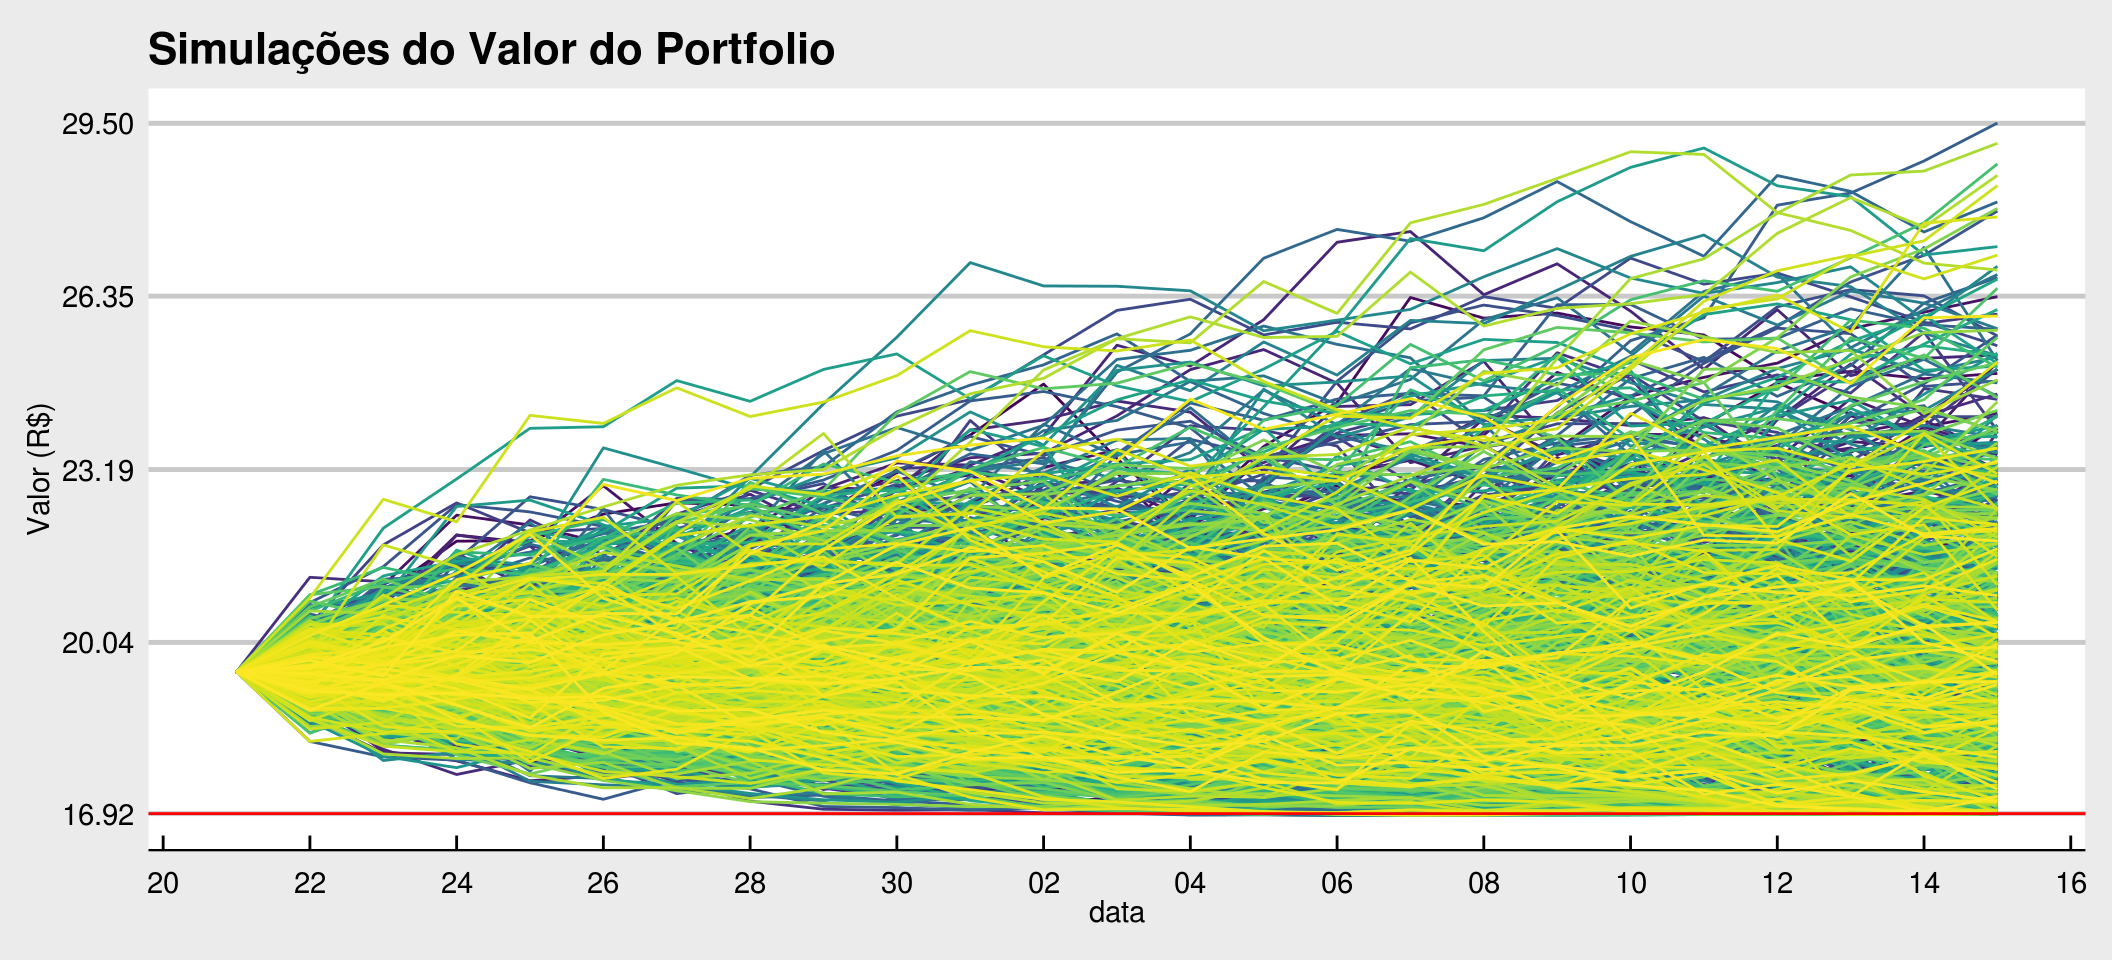
\includegraphics{91-monte-carlo_files/figure-latex/gr_port-1.pdf}

Ou seja, ao custo de 0.62\% do preço da ação, compramos uma proteção
contra uma queda de preços com probabilidade de 13.4\%.

Esta é apenas uma (simples) aplicação das inúmeras possíveis que a
Simulação de Monte Carlo possui no mundo das finanças. A SMC é uma
poderosa ferramenta para avaliação e controle de risco de grandes
portfólios, com centenas ou milhares de ativos, onde nem sempre
consegue-se aferir medidas de retorno esperado ou de risco de mercado de
forma analítica.

\bibliography{library.bib}


\end{document}
